% Format teze zasnovan je na paketu memoir
% http://tug.ctan.org/macros/latex/contrib/memoir/memman.pdf ili
% http://texdoc.net/texmf-dist/doc/latex/memoir/memman.pdf
% 
% Prilikom zadavanja klase memoir, navedenim opcijama se podešava 
% veličina slova (12pt) i jednostrano štampanje (oneside).
% Ove parametre možete menjati samo ako pravite nezvanične verzije
% mastera za privatnu upotrebu (na primer, u b5 varijanti ima smisla 
% smanjiti 
\documentclass[12pt,oneside]{memoir} 

% Ukljuceni paketi
\usepackage{amssymb}
\usepackage{amsmath}
\usepackage{amsfonts}
\usepackage{amsthm}
\usepackage{algorithm}
\usepackage{gensymb}
\usepackage[noend]{algpseudocode}
\usepackage{tikz}
\usetikzlibrary{arrows.meta}
\usepackage{pgfplots}
\pgfplotsset{width=7cm, compat=1.9, every tick label/.append style={font=\scriptsize}}
\usepgfplotslibrary{external}
\tikzexternalize

% Teoreme, definicije
\newtheorem{theorem}{Teorema}
\newtheorem{lemma}{Lema}
\newtheorem{corrolary}{Posledica}
\newtheorem{example}{Primer}

\theoremstyle{definition}
\newtheorem*{definition}{Definicija}

\makeatletter
\renewcommand*{\ALG@name}{Algoritam}
\makeatother

% Tikz stilovi
\tikzstyle{point}=[circle, fill,thick]
\tikzstyle{pointred}=[circle, fill=red!50,thick]
\tikzstyle{pointgreen}=[circle, fill=green!50,thick]
\tikzstyle{pointblue}=[circle, fill=blue!50,thick]
\tikzstyle{arrow}=[draw=black, >={Latex[length=2mm]}]
\tikzstyle{cover}=[draw, opacity=.2, line cap=round, line
join=round, line width=22pt]

\pgfplotscreateplotcyclelist{mylist}{%
cyan!80!black,mark=square*\\%
red!90!black,mark=square*\\%
blue,mark=*\\%
orange,mark=*\\%
green!80!black,mark=diamond*\\%
}

% Definisane komande
\def\CC{{C\nolinebreak[4]\hspace{-.05em}\raisebox{.4ex}{\tiny\bf ++}}}

\makeatletter
\def\blfootnote{\gdef\@thefnmark{}\@footnotetext}
\makeatother


% Paket koji definiše sve specifičnosti master rada Matematičkog fakulteta
\usepackage[latinica]{matfmaster} 
%
% Podrazumevano pismo je ćirilica.
%   Ako koristite pdflatex, a ne xetex, sav latinički tekst na srpskom jeziku
%   treba biti okružen sa \lat{...} ili \begin{latinica}...\end{latinica}.
%
% Opicija [latinica]:
%   ako želite da pišete latiniciom, dodajte opciju "latinica" tj.
%   prethodni paket uključite pomoću: \usepackage[latinica]{matfmaster}.
%   Ako koristite pdflatex, a ne xetex, sav ćirilički tekst treba biti
%   okružen sa \cir{...} ili \begin{cirilica}...\end{cirilica}.
%
% Opcija [biblatex]:
%   ako želite da koristite reference na više jezika i umesto paketa
%   bibtex da koristite BibLaTeX/Biber, dodajte opciju "biblatex" tj.
%   prethodni paket uključite pomoću: \usepackage[biblatex]{matfmaster}
%
% Opcija [b5paper]:
%   ako želite da napravite verziju teze u manjem (b5) formatu, navedite
%   opciju "b5paper", tj. prethodni paket uključite pomoću: 
%   \usepackage[b5paper]{matfmaster}. Tada ima smisla razmisliti o promeni
%   veličine slova (izmenom opcije 12pt na 11pt u \documentclass{memoir}).
%
% Naravno, opcije je moguće kombinovati.
% Npr. \usepackage[b5paper,biblatex]{matfmaster}

% Pomoćni paket koji generiše nasumičan tekst u kojem se javljaju sva slova
% azbuke (nema potrebe koristiti ovo u pravim disertacijama)
% \usepackage[latinica]{pangrami}

% Datoteka sa literaturom u BibTex tj. BibLaTeX/Biber formatu
\bib{master}

% Ime kandidata na srpskom jeziku (u odabranom pismu)
\autor{Ivan Drecun}
% Naslov teze na srpskom jeziku (u odabranom pismu)
\naslov{Algoritmi za ispitivanje izomorfizma grafova}
% Godina u kojoj je teza predana komisiji
\godina{2021}
% Ime i afilijacija mentora (u odabranom pismu)
\mentor{dr Filip \textsc{Marić}, vanredni profesor\\ Univerzitet u Beogradu, Matematički fakultet}
% Ime i afilijacija prvog člana komisije (u odabranom pismu)
\komisijaA{dr Miodrag \textsc{Živković}, redovan profesor\\ Univerzitet u Beogradu, Matematički fakultet}
% Ime i afilijacija drugog člana komisije (u odabranom pismu)
\komisijaB{dr Vesna \textsc{Marniković}, docent\\ Univerzitet u Beogradu, Matematički fakultet}
% Ime i afilijacija trećeg člana komisije (opciono)
% \komisijaC{}
% Ime i afilijacija četvrtog člana komisije (opciono)
% \komisijaD{}
% Datum odbrane (odkomentarisati narednu liniju i upisati datum odbrane ako je poznat)
% \datumodbrane{}

% Apstrakt na srpskom jeziku (u odabranom pismu)
\apstr{%
	Apstrakt rada.
}

% Ključne reči na srpskom jeziku (u odabranom pismu)
\kljucnereci{ključne, reči}

\begin{document}
% ==============================================================================
% Uvodni deo teze
\frontmatter
% ==============================================================================
% Naslovna strana
\naslovna
% Strana sa podacima o mentoru i članovima komisije
\komisija
% Strana sa posvetom (u odabranom pismu)
\posveta{Mami, tati i dedi}
% Strana sa podacima o disertaciji na srpskom jeziku
\apstrakt
% Sadržaj teze
\tableofcontents*

% ==============================================================================
% Glavni deo teze
\mainmatter
% ==============================================================================

% ------------------------------------------------------------------------------
\chapter{Uvod}
% ------------------------------------------------------------------------------

 Dva grafa su izomorfna ukoliko su jednaki do na promenu imenovanja čvorova.
 Problem ispitivanja izomorfizma grafova \textbf{GI} je problem određivanja
 postojanja takvog preimenovanja. Trenutno nije poznat algoritam polinomijalne
 vremenske složenosti koji rešava ovaj problem u opštem slučaju \cite{Babai}.
 Ipak, sa praktičnog stanovišta bi se moglo kazati da je problem rešen.
 Najuspešniji rešavači za \textbf{GI} (nauty \cite{McKay1,McKay}, Traces
 \cite{Piperno,McKay}, bliss \cite{Bliss}, conauto \cite{Conauto}, saucy
 \cite{Saucy}) sposobni su da reše velike instance teških klasa grafova u
 realnom vremenu. Pritom, sastavljanje teških klasa grafova za ove rešavače
 nije trivijalno i u realnoj upotrebi se takvi grafovi veoma retko javljaju. Na
 grafovima bez konkretne kombinatorne strukture se ti algoritmi čak ponašaju
 linearno \cite{Benchmark}.

 Postoje dva pristupa praktičnom rešavanju problema izomorfizma grafova. Prvi,
 neposredniji pristup je direktna pretraga izomorfizma između dva zadata grafa.
 Algoritmi zasnovani na ovom pristupu imaju korisnu osobinu da je moguće
 prekinuti pretragu pre ispitivanja velikog dela prostora pretrage, na primer
 kada je izomorfizam pronađen ili kada je pronađeno neko svojstvo grafova iz
 kog je moguće zaključiti njihov neizomorfizam. Drugi pristup oslanja se na
 mogućnost svođenja grafa na neki kanonski oblik. Time je omogućena jednostavna
 provera izomorfizma dva grafa - ispitivanjem jednakosti tako dobijenih
 kanonskih grafova. Ovakav pristup je znatno pogodniji od prvog u situacijama
 kada je neophodno efikasno ispitivanje izomorfizma u radu sa većim brojem
 grafova, na primer ukoliko je potrebno odrediti sve parove izomorfnih grafova
 u nekoj kolekciji grafova.  Uprkos tome što algoritmi za određivanje kanonske
 forme grafa ne poseduju mogućnost ranijeg zaustavljanja pretrage, neki od
 najuspešnijih modernih alata za rešavanje \textbf{GI} zasnovani su upravo na
 tom pristupu. 

 Centralna tema ovog rada je Mekejev algoritam za određivanje kanonske forme.
 Pojmovi i tvrđenja uvedeni su u skladu sa opisom opšteg okvira za konstrukciju
 algoritma prikazanim u radu \cite{McKay} na osnovu kog je zatim konstruisan
 konkretan algoritam. Uvedeno je i originalno uopštenje algoritma i prikazani
 su rezultati vremena izvršavanja implementiranog algoritma sa i bez tog
 uopštenja.

% ------------------------------------------------------------------------------
\chapter{Opšti algoritam}
% ------------------------------------------------------------------------------

 U ovoj glavi predstavljeni su osnovni matematički pojmovi neophodni za dalje
 razumevanje konstrukcije opšteg algoritma za određivanje kanonske forme grafa.
 Uvedeni su pojmovi \emph{bojenja} i \emph{obojenog grafa}, nakon čega je
 prikazana konstrukcija stabla pretrage koja leži u osnovi algoritma. Nad
 stablom je pogodno definisana invarijanta koja omogućava određivanje grupe
 automorfizama grafa i kanonske forme. Na kraju su prikazani i mehanizmi
 odsecanja pretrage koji omogućavaju praktično izvršavanje algoritma u razumnom
 vremenu.

 \section{Osnovni pojmovi}

  \subsection{Permutacija i particija}

   \emph{Permutacija} konačnog skupa $A$ je bilo koja bijekcija $g : A \to A$.
   Skup svih takvih permutacija označavamo sa $S_A$. Specijalno, ako je $A =
   \{1, 2, \dots, n\}$ za neki prirodan broj $n$, tada koristimo oznaku $S_n$.
   Zajedno sa operacijom kompozicije preslikavanja skup $S_n$ je grupa koju
   zovemo \emph{simetrična grupa stepena $n$}. Identičnu permutaciju označavamo
   sa $id$, a inverz permutacije $g$ sa $g^{-1}$. Permutaciju $g$ možemo
   zapisati kao preslikavanje, npr.  $g : \begin{pmatrix} 1 & 2 & 3 & 4 & 5\\ 3
   & 4 & 1 & 5 & 2 \end{pmatrix}$ ili kao kompoziciju ciklusa $(1\ 3)(2\ 4\ 5)$.

   \emph{Particija} konačnog skupa $A$ je skup nepraznih podskupova od $A$
   takav da se svaki element skupa $A$ nalazi u tačno jednom od tih podskupova.
   Te podskupove zovemo \emph{klasama} ili \emph{ćelijama} particije. Relacija
   $\approx$ na skupu $A$ je \emph{relacija ekvivalencije} ukoliko je
   refleksivna, simetrična i tranzitivna. \emph{Klasa ekvivalencije} elementa
   $a \in A$ je skup $C_a = \{b \in A \mid a \approx b\}$. Skup klasa
   ekvivalencije relacije $\approx$ čini jednu particiju $P = A/{\approx}$ skupa
   $A$. Slično, svaka particija $P$ je skup klasa ekvivalencije jedne relacije
   ekvivalencije $\approx_P$. Zbog ovoga u daljem tekstu poistovećujemo pojmove
   particije skupa $A$ i relacije ekvivalencije na skupu $A$.

   Neka su $\alpha$ i $\beta$ particije skupa $A$. Particija $\alpha$
   je \emph{finija} od particije $\beta$ (u oznaci ${\alpha} \leq {\beta}$)
   ukoliko za sve $a, b \in A$ važi $a \approx_\alpha b \implies a \approx_\beta b$.
   Ovaj uslov je ekvivalentan tome da je svaka klasa particije $\alpha$
   podskup neke klase particije $\beta$.

   Neka su $\alpha$ i $\beta$ particije skupa $A$. Particija $\alpha \lor
   \beta$ definisana kao tranzitivno zatvorenje relacije $a \approx b \iff a
   \approx_\alpha b \lor a \approx_\beta b$, odnosno $a \approx_{\alpha \lor
   \beta} b \iff x_1 \approx x_2 \approx \dots \approx x_k$ za neke $a = x_1,
   x_2, \dots, x_k = b$ naziva se \emph{supremum particija $\alpha$ i $\beta$}.
   Primetimo da su particije $\alpha$ i $\beta$ finije od $\alpha \lor \beta$,
   kao i da je $\alpha \lor \beta$ finije od svakog $\gamma$ za koje važi
   $\alpha, \beta \leq \gamma$, odnosno da je $\alpha \lor \beta$ zaista
   njihovo najmanje gornje ograničenje.

   \begin{example}
	   Na slici \ref{img:partition} prikazane su dve particije skupa od šest
	   elemenata, kao i njihov supremum. Sa slike se vidi i da su obe particije
	   finije od supremuma.
   \end{example}

   \begin{figure}[htp]
	   \centering
	   \begin{tikzpicture}
		   \begin{scope}
			   \node (0) at (1, 0)[point] {};
			   \node (1) at (0.5, 0.86)[point] {};
			   \node (2) at (-0.5, 0.86)[point] {};
			   \node (3) at (-1, 0)[point] {};
			   \node (4) at (-0.5, -0.86)[point] {};
			   \node (5) at (0.5, -0.86)[point] {};
		   \end{scope}
		   \begin{scope}
			   \draw[edge, cover] (1.center) -- (2.center);
			   \draw[edge, cover] (3.center) -- (4.center);
			   \draw[edge, cover] (0.center) -- (0.center);
			   \draw[edge, cover] (5.center) -- (5.center);
		   \end{scope}
	   \end{tikzpicture}
	   \hspace{20pt}
	   \begin{tikzpicture}
		   \begin{scope}
			   \node (0) at (1, 0)[point] {};
			   \node (1) at (0.5, 0.86)[point] {};
			   \node (2) at (-0.5, 0.86)[point] {};
			   \node (3) at (-1, 0)[point] {};
			   \node (4) at (-0.5, -0.86)[point] {};
			   \node (5) at (0.5, -0.86)[point] {};
		   \end{scope}
		   \begin{scope}
			   \draw[edge, cover] (1.center) -- (1.center);
			   \draw[edge, cover] (2.center) -- (3.center);
			   \draw[edge, cover] (0.center) -- (5.center);
			   \draw[edge, cover] (4.center) -- (4.center);
		   \end{scope}
	   \end{tikzpicture}
	   \hspace{20pt}
	   \begin{tikzpicture}
		   \begin{scope}
			   \node (a0) at (1, 0)[point] {};
			   \node (a1) at (0.5, 0.86)[point] {};
			   \node (a2) at (-0.5, 0.86)[point] {};
			   \node (a3) at (-1, 0)[point] {};
			   \node (a4) at (-0.5, -0.86)[point] {};
			   \node (a5) at (0.5, -0.86)[point] {};
		   \end{scope}
		   \begin{scope}
			   \draw[edge, cover] (a1.center) -- (a2.center) -- (a3.center) --
			   (a4.center) -- (a1.center) -- (a3.center) -- (a2.center) -- (a4.center);
			   \draw[edge, cover] (a0.center) -- (a5.center);
		   \end{scope}
	   \end{tikzpicture}
	   \caption{Particije (levo) i supremum (desno).}
	   \label{img:partition}
   \end{figure}

  \subsection{Obojen graf}

   \emph{Bojenje} skupa $A$ je surjekcija $\pi : A \to \{1, 2, \dots, k\}$ za
   neki prirodan broj $k > 0$. Označimo skup svih bojenja skupa sa $n$
   elemenata sa $\Pi_n$ (nadalje $\Pi$).  Broj $k$ zovemo \emph{brojem boja} i
   označavamo ga sa $|\pi|$.  \emph{Ćelija bojenja} $\pi$ boje $c$ je skup svih
   čvorova te boje, odnosno $\pi^{-1}(c)$ za $c \in \{1, 2, ..., k\}$.  Bojenje
   je \emph{diskretno} ukoliko je $|\pi| = n$ i tada je $\pi$ permutacija skupa
   $A$.

   Označimo sa $\sim_\pi$ binarnu relaciju na skupu $A$ definisanu sa $a
   \sim_\pi b \iff \pi(a) = \pi(b)$. U pitanju je jedinstvena particija čije
   klase odgovaraju upravo ćelijama bojenja $\pi$ i nazivamo je \emph{particija
   bojenja} $\pi$. Primetimo da nije moguće poistovetiti bojenje i particiju
   zato što za proizvoljnu particiju bojenje čije ćelije odgovaraju klasama
   particije nije jedinstveno - postoji ih onoliko koliko je različitih
   rasporeda klasa.  Bojenje možemo poistovetiti sa \emph{uređenom particijom},
   odnosno particijom čije su klase uređene u niz.

   Bojenje $\pi_1$ je \emph{finije} od bojenja $\pi_2$ (u oznaci $\pi_1 \leq \pi_2$)
   ukoliko za sve $a, b \in A$ važi implikacija $\pi_2(a) < \pi_2(b) \implies
   \pi_1(a) < \pi_1(b)$.  Primetimo da za bojenja $\pi_1$ i $\pi_2$ važi $\pi_1
   \leq \pi_2 \implies {\sim_{\pi_1}} \leq {\sim_{\pi_2}}$, ali ne i obrnuto.

   \begin{example}
	   Neka je $\pi :
	   \begin{pmatrix}
		   1 & 2 & 3 & 4 & 5 & 6 \\
		   3 & 1 & 2 & 2 & 1 & 2
	   \end{pmatrix}$
	   jedno bojenje. Koristan je zapis po ćelijama bojenja $\pi = [2\ 5 \mid
	   4\ 3\ 6 \mid 1]$, pri čemu redosled brojeva unutar ćelija nije bitan.
	   Bojenje $\pi_1 = [5 \mid 2 \mid 4\ 6 \mid 3 \mid 1]$ je finije od $\pi$.
	   Bojenje $\pi_2 = [2 \mid 3 \mid 4\ 6 \mid 5 \mid 1]$ nije finije od
	   $\pi$ iako važi da je svaka njegova ćelija podskup neke ćelije bojenja
	   $\pi$. To je moguće videti iz toga što se bojenje $\pi$ može dobiti
	   spajanjem susednih ćelija bojenja $\pi_1$, ali ne i spajanjem susednih
	   ćelija bojenja $\pi_2$.
   \end{example}

   \begin{example}
	   Neka je $\pi = [4 \mid 1 \mid 3 \mid 2]$ diskretno bojenje. Odgovarajuća
	   permutacija je $\pi :
	   \begin{pmatrix}
		   1 & 2 & 3 & 4 \\
		   2 & 4 & 3 & 1
	   \end{pmatrix}$,
	   a njen inverz je $\pi^{-1} :
	   \begin{pmatrix}
		   1 & 2 & 3 & 4 \\
		   4 & 1 & 3 & 2
	   \end{pmatrix}$.
   \end{example}

   \emph{Graf} $G = (V, E)$ je uređeni par konačnog \emph{skupa čvorova} $V$ i
   \emph{skupa grana} $E \subseteq V \times V$ pri čemu za sve $u, v \in V$
   važi $(v, v) \notin E$ i ako je $(u, v) \in E$ onda je $(v, u) \in E$. U
   nastavku pretpostavljamo da je $V = \{1, 2, \dots, n\}$ za neki prirodan
   broj $n > 0$. Označimo skup svih grafova sa $n$ čvorova sa $\mathcal{G}_n$
   (nadalje $\mathcal{G}$).

   \emph{Matrica povezanosti grafa} je preslikavanje $\psi : \mathcal{G} \times
   V \times V \to \{0, 1\}$ takvo da važi $\psi(G, u, v) = 1 \iff (u, v) \in
   E$.  \emph{Binarna reprezentacija $bin(G)$ grafa} $G$ je binarni niz dobijen
   nadovezivanjem redova gornjeg trougla matrice povezanosti grafa $G$.

   \emph{Obojen graf} je uređeni par $(G, \pi)$ gde je $\pi$ jedno bojenje
   skupa čvorova $V$ grafa $G$. Kažemo i da je $\pi$ \emph{bojenje grafa} $G$.

   \begin{example}
	   Na slici \ref{img:matrix} je prikazan jedan graf $G$ zajedno sa njegovom
	   matricom povezanosti. Njegova binarna reprezentacija je $bin(G) =
	   101011$.
   \end{example}

   \begin{figure}[htp]
	   \centering
	   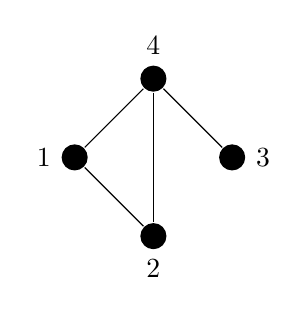
\begin{tikzpicture}
		   \begin{scope}
			   \node (0) at (0, 0)[point, label=180:1] {};
			   \node (1) at (1, 1)[point, label=90:4] {};
			   \node (2) at (2, 0)[point, label=0:3] {};
			   \node (3) at (1, -1)[point, label=-90:2] {};
		   \end{scope}
		   \begin{scope}
			   \path [-] (0) edge (1);
			   \path [-] (1) edge (2);
			   \path [-] (1) edge (3);
			   \path [-] (0) edge (3);
		   \end{scope}
	   \end{tikzpicture}
	   \hspace{20pt}
	   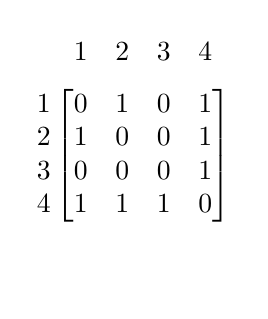
\begin{tikzpicture}
		   \node at (0, 0.6)[] {};
		   \node at (0, 3.5)[] {$\ \ \begin{matrix} 1 & 2 & 3 & 4 \end{matrix}$};
		   \node at (0, 2.2)[] {
		   $ \begin{matrix}
			   1 \\
			   2 \\
			   3 \\
			   4
			 \end{matrix}
			 \begin{bmatrix}
			   0 & 1 & 0 & 1 \\
			   1 & 0 & 0 & 1 \\
			   0 & 0 & 0 & 1 \\
			   1 & 1 & 1 & 0
		     \end{bmatrix}$
		   };
	   \end{tikzpicture}
	   \caption{Graf i matrica povezanosti.}
	   \label{img:matrix}
   \end{figure}


   \subsection{Generatori i dejstvo grupe}

   Neka je $G$ grupa i $H$ podskup od $G$. Tada sa $\langle H \rangle$
   označavamo minimalnu podgrupu grupe $G$ koja sadrži sve elemente skupa $H$ i
   kažemo da je ona \emph{generisana elementima skupa $H$}. Ukoliko je $H =
   \{g_1, \dots, g_n\}$ za neki prirodan broj $n$, koristimo i oznaku $\langle
   g_1, \dots, g_n \rangle$.

   Neka je nad grupom $G$ i skupom $S$ definisano dejstvo. Dejstvo elementa
   grupe $g \in G$ na element skupa $s \in S$ označavamo sa $gs$ ili $s^g$, pri
   čemu ako su $g_1, g_2 \in G$ tada je $(g_1g_2)s = g_1(g_2s)$ odnosno
   $s^{g_1g_2} = (s^{g_2})^{g_1}$.  \emph{Orbita} elementa $s$ je skup
   $\Omega_s^G = \{s^g \mid g \in G\}$.  \emph{Stabilizator} elementa $s$ je
   skup $\Sigma_s^G = \{g \in G \mid s^g=s\}$ koji čini jednu podgrupu od $G$.

   Na skupu čvorova $V$ definisano je dejstvo grupe $S_n$ sa $v^g = g(v)$ za $v
   \in V$ i $g \in S_n$.  Definiciju dejstva grupe permutacija možemo proširiti
   i na složenije strukture:
   \begin{itemize}
       \item $W^g = \{w^g \mid w \in W\}$ za skup $W \subseteq V$
       \item $w^g = (v_1^g, v_2^g, \dots, v_k^g)$ za uređenu $k$-torku $w$
       \item $G^g = (V, E')$ za graf $G$ i $E' = \{e^g \mid e \in E\}$
       \item Ako je $\pi$ bojenje, $\pi^g$ je bojenje za koje važi
		   $\pi^g(v^g)=\pi(v)$ odnosno $\pi^g=\pi g^{-1}$
       \item $(G, \pi)^g = (G^g, \pi^g)$ za obojen graf $(G, \pi)$
   \end{itemize}
   Primetimo da za ćeliju bojenja $\pi^{-1}(c)$ važi $\pi^{-1}(c)^g =
   (\pi^g)^{-1}(c)$. To je zato što $(\pi^g)^{-1}(c) = \{v \mid \pi^g(v) = c\}
   = \{w^g \mid \pi^g(w^g) = c\} = \{w^g \mid \pi(w) = c\} = \pi^{-1}(c)^g$. 

   \begin{example}
	   Na slici \ref{img:action} prikazani su obojeni grafovi $(G, \pi)$ i $(G^g,
	   \pi^g)$ za $g : \begin{pmatrix} 1 & 2 & 3\\ 3 & 1 & 2\end{pmatrix}$.
   \end{example}
   \begin{figure}[htp]
	   \centering
	   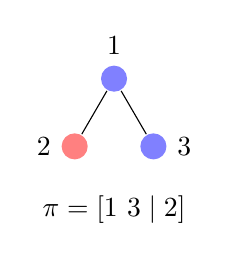
\begin{tikzpicture}
		   \begin{scope}
			   \node (2) at (0, 0)[pointred, label=180:2] {};
			   \node (1) at (0.5, 0.86)[pointblue, label=90:1] {};
			   \node (3) at (1, 0)[pointblue, label=0:3] {};
			   \node (p) at (0.5, -0.8) {
				   $\pi = [1 \ 3 \mid 2]$
			   };
		   \end{scope}
		   \begin{scope}
			   \path [-] (1) edge (2);
			   \path [-] (1) edge (3);
		   \end{scope}
	   \end{tikzpicture}
	   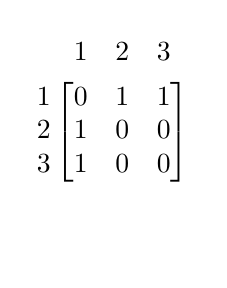
\begin{tikzpicture}
		   \node (0) at (0, 0) {};
		   \node (a) at (0, 2.5) {$\ \ \begin{matrix}1 & 2 & 3\end{matrix}$};
		   \node (m) at (0, 1.5) {
			   $\begin{matrix}
				   1\\ 2\\ 3
			   	\end{matrix}
			   	\begin{bmatrix}
				   0 & 1 & 1\\
				   1 & 0 & 0\\
				   1 & 0 & 0
			   	\end{bmatrix}$
		   };
	   \end{tikzpicture}
	   \hspace{10pt}
	   \begin{tikzpicture}
		   \node (1) at (0, -1) {};
		   \node (0) at (0, 0) {$\longrightarrow$};
		   \node (g) at (0, 0.5) {$g$};
	   \end{tikzpicture}
	   \hspace{10pt}
	   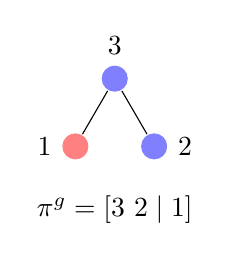
\begin{tikzpicture}
		   \begin{scope}
			   \node (2) at (0, 0)[pointred, label=180:1] {};
			   \node (1) at (0.5, 0.86)[pointblue, label=90:3] {};
			   \node (3) at (1, 0)[pointblue, label=0:2] {};
			   \node (p) at (0.5, -0.8) {
				   $\pi^g = [3 \ 2 \mid 1]$
			   };
		   \end{scope}
		   \begin{scope}
			   \path [-] (1) edge (2);
			   \path [-] (1) edge (3);
		   \end{scope}
	   \end{tikzpicture}
	   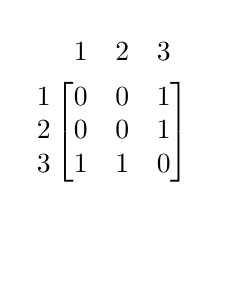
\begin{tikzpicture}
		   \node (0) at (0, 0) {};
		   \node (a) at (0, 2.5) {$\ \ \begin{matrix}1 & 2 & 3\end{matrix}$};
		   \node (m) at (0, 1.5) {
			   $\begin{matrix}
				   1\\ 2\\ 3
			   	\end{matrix}
			   	\begin{bmatrix}
				   0 & 0 & 1\\
				   0 & 0 & 1\\
				   1 & 1 & 0
			   	\end{bmatrix}$
		   };
	   \end{tikzpicture}
	   \caption{Obojeni grafovi $(G, \pi)$ i $(G^g, \pi^g)$.}
	   \label{img:action}
   \end{figure}

   \subsection{Izomorfizam}

   Obojeni grafovi $(G_1, \pi_1)$ i $(G_2, \pi_2)$ su \emph{izomorfni} (u oznaci
   $(G_1, \pi_1) \cong (G_2, \pi_2)$) ukoliko postoji $g \in S_n$ tako da je
   $(G_1, \pi_1) = (G_2, \pi_2)^g$. Takvo $g$ zovemo \emph{izomorfizam}.

   \begin{example}
	   Neka su dati grafovi $(G_1, \pi_1)$ i $(G_2, \pi_2)$ kao na slici
	   \ref{img:iso}. Ako je redosled boja crvena, zelena, plava, tada je
	   $\pi_1 = [1\ 4\mid 2 \mid 3]$ i $\pi_2 = [3\ 1 \mid 4 \mid 2]$. Ovi
	   grafovi su izomorfni za izomorfizam
	   $g :
	   \begin{pmatrix}
		   1 & 2 & 3 & 4\\
		   3 & 4 & 2 & 1
	   \end{pmatrix}$.
   \end{example}
   \begin{figure}[htp]
	   \centering
	   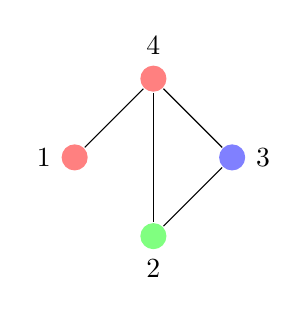
\begin{tikzpicture}
		   \begin{scope}
			   \node (0) at (0, 0)[pointred, label=180:1] {};
			   \node (1) at (1, 1)[pointred, label=90:4] {};
			   \node (2) at (2, 0)[pointblue, label=0:3] {};
			   \node (3) at (1, -1)[pointgreen, label=-90:2] {};
		   \end{scope}
		   \begin{scope}
			   \path [-] (0) edge (1);
			   \path [-] (1) edge (2);
			   \path [-] (1) edge (3);
			   \path [-] (2) edge (3);
		   \end{scope}
	   \end{tikzpicture}
	   \hspace{20pt}
	   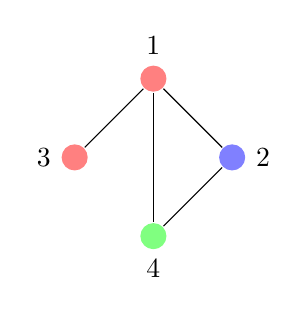
\begin{tikzpicture}
		   \begin{scope}
			   \node (0) at (0, 0)[pointred, label=180:3] {};
			   \node (1) at (1, 1)[pointred, label=90:1] {};
			   \node (2) at (2, 0)[pointblue, label=0:2] {};
			   \node (3) at (1, -1)[pointgreen, label=-90:4] {};
		   \end{scope}
		   \begin{scope}
			   \path [-] (0) edge (1);
			   \path [-] (1) edge (2);
			   \path [-] (1) edge (3);
			   \path [-] (2) edge (3);
		   \end{scope}
	   \end{tikzpicture}
	   \caption{Izomorfni grafovi $(G_1, \pi_1)$ i $(G_2, \pi_2)$.}
	   \label{img:iso}
   \end{figure}

   \emph{Automorfizam} obojenog grafa $(G, \pi)$ je izomorfizam tog grafa sa
   samim sobom, odnosno $g \in S_n$ za koje važi $(G, \pi) = (G, \pi)^g$. Skup
   automorfizama grafa $(G, \pi)$ označavamo sa $Aut(G, \pi)$. Zajedno sa
   operacijom kompozicije preslikavanja skup $Aut(G, \pi)$ čini \emph{grupu
   automorfizama}.

   \begin{example}
	   Na slici \ref{img:aut} prikazan je graf sa jednim automorfizmom.
   \end{example}

   \begin{figure}[htp]
	   \centering
	   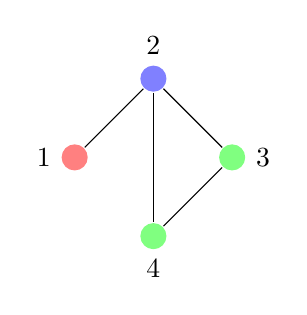
\begin{tikzpicture}
		   \begin{scope}
			   \node (0) at (0, 0)[pointred, label=180:1] {};
			   \node (1) at (1, 1)[pointblue, label=90:2] {};
			   \node (2) at (2, 0)[pointgreen, label=0:3] {};
			   \node (3) at (1, -1)[pointgreen, label=-90:4] {};
		   \end{scope}
		   \begin{scope}
			   \path [-] (0) edge (1);
			   \path [-] (1) edge (2);
			   \path [-] (1) edge (3);
			   \path [-] (2) edge (3);
		   \end{scope}
	   \end{tikzpicture}
	   \caption{Graf sa automorfizmom 
	   $g :
	   \begin{pmatrix}
		   1 & 2 & 3 & 4\\
		   1 & 2 & 4 & 3
	   \end{pmatrix}$
       .}
	   \label{img:aut}
   \end{figure}


   \subsection{Kanonska forma}

   Neka je $f : \mathcal{G} \times \Pi \to S$ preslikavanje iz skupa svih
   obojenih grafova u proizvoljan skup $S$.  Kažemo da je $f$ \emph{funkcija
   invarijantna na imenovanje čvorova} ukoliko za svaki obojen graf $(G, \pi)$
   i svaku permutaciju $g \in S_n$ važi $f(G^g, \pi^g) = f(G, \pi)$.
   Neformalno, to znači da vrednost funkcije $f$ ne zavisi od konkretnog
   imenovanja čvorova grafa, već samo od njegove unutrašnje strukture.

   Ako na skupu $S$ postoji definisano dejstvo grupe $S_n$, kažemo da je $f$
   \emph{transformacija invarijantna na imenovanje čvorova} ukoliko za svaki
   obojen graf $(G, \pi)$ i svaku permutaciju $g \in S_n$ važi $f(G^g, \pi^g) =
   f(G, \pi)^g$.


   \begin{definition}
	   \emph{Kanonska forma} je preslikavanje $\mathcal{C} : \mathcal{G} \times \Pi \to
	   \mathcal{G} \times \Pi$ koje ispunjava sledeće uslove:
	   \begin{itemize}
		   \item[($\mathcal{C}1$)] Za svaki obojen graf $(G, \pi)$ važi
			   $\mathcal{C}(G, \pi) \cong (G,
			\pi)$
		\item[($\mathcal{C}2$)] $\mathcal{C}$ je funkcija invarijantna na
			imenovanje čvorova
	   \end{itemize}
   \end{definition}

   \begin{example}
	   Neka je definisano uređenje na skupu obojenih grafova leksikografskim
	   poređenjem odgovarajućih nizova $(bin(G), \pi(1), \dots, \pi(n))$. Tada
	   je preslikavanje definisano sa $\mathcal{M}(G, \pi) = \max_{g \in S_n}
	   (G^g, \pi^g)$ kanonska forma. Na slici \ref{img:maxcanon} prikazane su
	   sve permutacije jednog obojenog grafa i istaknut je maksimum u prethodno
	   opisanom smislu.
   \end{example}
   \begin{figure}[htp]
	   \centering
	   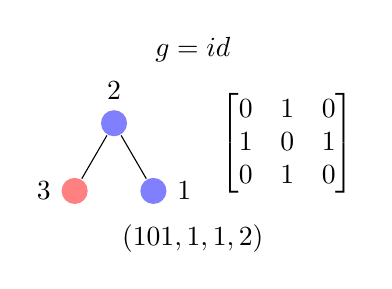
\begin{tikzpicture}
		   \begin{scope}
			   \node (g) at (1.5, 1.8) {$g = id$};
			   \node (3) at (0, 0)[pointred, label=180:3] {};
			   \node (2) at (0.5, 0.86)[pointblue, label=90:2] {};
			   \node (1) at (1, 0)[pointblue, label=0:1] {};
			   \node (m) at (2.7, 0.6) {
				   $\begin{bmatrix}
					   0 & 1 & 0\\
					   1 & 0 & 1\\
					   0 & 1 & 0
				   \end{bmatrix}$
			   };
			   \node (v) at (1.5, -0.6) {
				   $(101, 1, 1, 2)$
			   };
		   \end{scope}
		   \begin{scope}
			   \path [-] (2) edge (1);
			   \path [-] (2) edge (3);
		   \end{scope}
	   \end{tikzpicture}
	   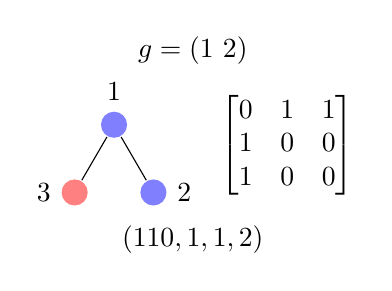
\begin{tikzpicture}
		   \begin{scope}
			   \node (g) at (1.5, 1.8) {$g = (1 \ 2)$};
			   \node (3) at (0, 0)[pointred, label=180:3] {};
			   \node (1) at (0.5, 0.86)[pointblue, label=90:1] {};
			   \node (2) at (1, 0)[pointblue, label=0:2] {};
			   \node (m) at (2.7, 0.6) {
				   $\begin{bmatrix}
					   0 & 1 & 1\\
					   1 & 0 & 0\\
					   1 & 0 & 0
				   \end{bmatrix}$
			   };
			   \node (v) at (1.5, -0.6) {
				   $(110, 1, 1, 2)$
			   };
		   \end{scope}
		   \begin{scope}
			   \path [-] (1) edge (2);
			   \path [-] (1) edge (3);
		   \end{scope}
	   \end{tikzpicture}
	   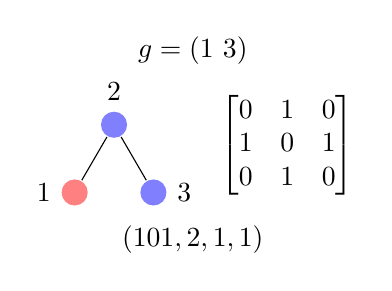
\begin{tikzpicture}
		   \begin{scope}
			   \node (g) at (1.5, 1.8) {$g = (1 \ 3)$};
			   \node (1) at (0, 0)[pointred, label=180:1] {};
			   \node (2) at (0.5, 0.86)[pointblue, label=90:2] {};
			   \node (3) at (1, 0)[pointblue, label=0:3] {};
			   \node (m) at (2.7, 0.6) {
				   $\begin{bmatrix}
					   0 & 1 & 0\\
					   1 & 0 & 1\\
					   0 & 1 & 0
				   \end{bmatrix}$
			   };
			   \node (v) at (1.5, -0.6) {
				   $(101, 2, 1, 1)$
			   };
		   \end{scope}
		   \begin{scope}
			   \path [-] (2) edge (1);
			   \path [-] (2) edge (3);
		   \end{scope}
	   \end{tikzpicture}

	   \vspace{10pt}

	   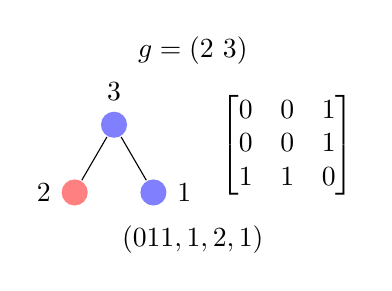
\begin{tikzpicture}
		   \begin{scope}
			   \node (g) at (1.5, 1.8) {$g = (2 \ 3)$};
			   \node (2) at (0, 0)[pointred, label=180:2] {};
			   \node (3) at (0.5, 0.86)[pointblue, label=90:3] {};
			   \node (1) at (1, 0)[pointblue, label=0:1] {};
			   \node (m) at (2.7, 0.6) {
				   $\begin{bmatrix}
					   0 & 0 & 1\\
					   0 & 0 & 1\\
					   1 & 1 & 0
				   \end{bmatrix}$
			   };
			   \node (v) at (1.5, -0.6) {
				   $(011, 1, 2, 1)$
			   };
		   \end{scope}
		   \begin{scope}
			   \path [-] (3) edge (1);
			   \path [-] (3) edge (2);
		   \end{scope}
	   \end{tikzpicture}
	   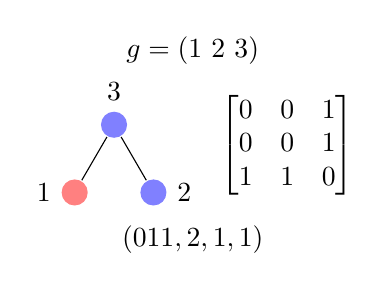
\begin{tikzpicture}
		   \begin{scope}
			   \node (g) at (1.5, 1.8) {$g = (1 \ 2 \ 3)$};
			   \node (1) at (0, 0)[pointred, label=180:1] {};
			   \node (3) at (0.5, 0.86)[pointblue, label=90:3] {};
			   \node (2) at (1, 0)[pointblue, label=0:2] {};
			   \node (m) at (2.7, 0.6) {
				   $\begin{bmatrix}
					   0 & 0 & 1\\
					   0 & 0 & 1\\
					   1 & 1 & 0
				   \end{bmatrix}$
			   };
			   \node (v) at (1.5, -0.6) {
				   $(011, 2, 1, 1)$
			   };
		   \end{scope}
		   \begin{scope}
			   \path [-] (3) edge (1);
			   \path [-] (3) edge (2);
		   \end{scope}
	   \end{tikzpicture}
	   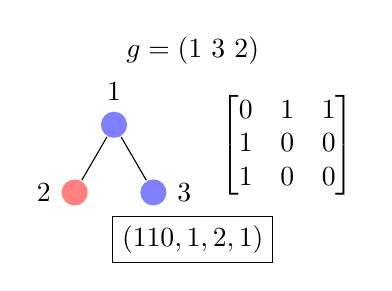
\begin{tikzpicture}
		   \begin{scope}
			   \node (g) at (1.5, 1.8) {$g = (1 \ 3 \ 2)$};
			   \node (2) at (0, 0)[pointred, label=180:2] {};
			   \node (1) at (0.5, 0.86)[pointblue, label=90:1] {};
			   \node (3) at (1, 0)[pointblue, label=0:3] {};
			   \node (m) at (2.7, 0.6) {
				   $\begin{bmatrix}
					   0 & 1 & 1\\
					   1 & 0 & 0\\
					   1 & 0 & 0
				   \end{bmatrix}$
			   };
			   \node (v)[draw=black] at (1.5, -0.6) {
				   $(110, 1, 2, 1)$
			   };
		   \end{scope}
		   \begin{scope}
			   \path [-] (1) edge (2);
			   \path [-] (1) edge (3);
		   \end{scope}
	   \end{tikzpicture}
	   \caption{Sve permutacije jednog obojenog grafa.}
	   \label{img:maxcanon}
   \end{figure}


 \section{Stablo pretrage}

  Označimo sa $V^*$ skup svih konačnih nizova elemenata skupa $V$. Ako je $\nu
  \in V^*$ sa $|\nu|$ označavamo dužinu niza $\nu$. Ako je $\nu = (v_1, v_2,
  \dots, v_k) \in V^*$ i $w \in V$, onda $\nu \| w$ označava niz $(v_1, v_2,
  \dots, v_k, w)$. Za $0 \leq s \leq k$ prefiks niza $\nu$ dužine $s$ označavamo
  sa $[\nu]_s = (v_1, v_2, \dots, v_s)$. Uređenje $\leq$ na skupu $V^*$
  predstavlja leksikografski poredak.

  Čvorovi stabla pretrage  predstavljeni su nizovima elemenata skupa $V$, pri
  čemu korenu stabla odgovara prazan niz. U nastavku definišemo funkcije na
  osnovu kojih ćemo opisati pravila grananja u stablu.

  \begin{definition}
   \emph{Funkcija profinjavanja} je bilo koje preslikavanje $R : \mathcal{G}
	  \times \Pi \times V^* \to \Pi$ koje za svaki obojen graf $(G, \pi)$ i
	  svako $\nu \in V^*$ zadovoljava sledeće uslove:
  
   \begin{itemize}
       \item[(R1)] $R(G, \pi, \nu) \leq \pi$
       \item[(R2)] Ako je $v \in \nu$, onda je $\{v\}$ ćelija bojenja $R(G,
     	  \pi, \nu)$
       \item[(R3)] Za svako $g \in S_n$ važi $R(G^g, \pi^g, \nu^g) = R(G,
     	 \pi, \nu)^g$
   \end{itemize}
  \end{definition}

  \begin{definition}
   \emph{Funkcija odabira ciljne ćelije} je bilo koje preslikavanje $T :
	  \mathcal{G} \times \Pi \times V^* \to \mathcal{P}(V)$ koje za svaki
	  obojen graf $(G, \pi)$ i svako $\nu \in V^*$ zadovoljava sledeće
	  uslove:
  
   \begin{itemize}
       \item[(T1)] Ako je $R(G, \pi, \nu)$ diskretno, onda je $T(G, \pi, \nu) =
     	  \emptyset$
       \item[(T2)] Ako $R(G, \pi, \nu)$ nije diskretno, onda je $T(G, \pi, \nu)$
     	  višečlana ćelija od $R(G, \pi, \nu)$
       \item[(T3)] Za svako $g \in S_n$ važi $T(G^g, \pi^g, \nu^g) = T(G, \pi,
     	 \nu)^g$
   \end{itemize}
  \end{definition}

  Kako je graf fiksan, ove funkcije možemo smatrati funkcijama čvorova stabla.
  Funkcija profinjavanja obezbeđuje postojanje bojenja pridruženog svakom čvoru
  stabla $\nu$, koje zbog uslova (R2) razdvaja sve čvorove grafa niza $\nu$ u
  zasebne ćelije. Funkcija odabira ciljne ćelije nam omogućava da odaberemo
  skup čvorova grafa koji nam služi za konstrukciju dece tog čvora u stablu.
  Treći uslov u obe definicije govori da su u pitanju transformacije
  invarijantne na imenovanje čvorova.

  \begin{definition}
      \emph{Stablo pretrage} $\mathcal{T}(G, \pi)$ određeno je sledećim uslovima:
  
   \begin{itemize}
       \item[($\mathcal{T}1$)] Koren stabla $\mathcal{T}(G, \pi)$ je prazan niz $()$
       \item[($\mathcal{T}2$)] Ako je $\nu$ čvor stabla $\mathcal{T}(G, \pi)$, njegova deca u
     	stablu su $\{$\nu$ \| w \mid w \in T(G, \pi, \nu)\}$
   \end{itemize}
  \end{definition}

  Iz definicije se vidi da je neki čvor list stabla ako i samo ako je njemu
  pridruženo bojenje diskretno. Primetimo da je ovako definisano stablo konačno
  zato što za svako $\nu$ koje je permutacija skupa $V$ važi da je bojenje
  pridruženo nekom njegovom prefiksu diskretno ili je njemu pridruženo bojenje
  diskretno.

  \begin{example}
	  Prikažimo jedno jednostavno stablo pretrage. Za funkciju odabira ciljne
	  ćelije možemo uzeti funkciju koja bira prvu višečlanu ćeliju bojenja.
	  Za funkciju profinjavanja možemo uzeti funkciju koja dodeljuje boje
	  čvorovima u skladu sa početnim bojenjem $\pi$, pri čemu čvorove niza
	  $\nu$ izdvaja u zasebne ćelije. Na slici \ref{img:tree} je prikazano
	  stablo pretrage jednog grafa.
  \end{example}

   \begin{figure}[htp]
	   \centering
	   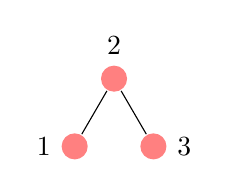
\begin{tikzpicture}
		   \begin{scope}
			   \node (1) at (0, 0)[pointred, label=180:1] {};
			   \node (2) at (0.5, 0.86)[pointred, label=90:2] {};
			   \node (3) at (1, 0)[pointred, label=0:3] {};
		   \end{scope}
		   \begin{scope}
			   \path [-] (1) edge (2);
			   \path [-] (2) edge (3);
		   \end{scope}
	   \end{tikzpicture}

	   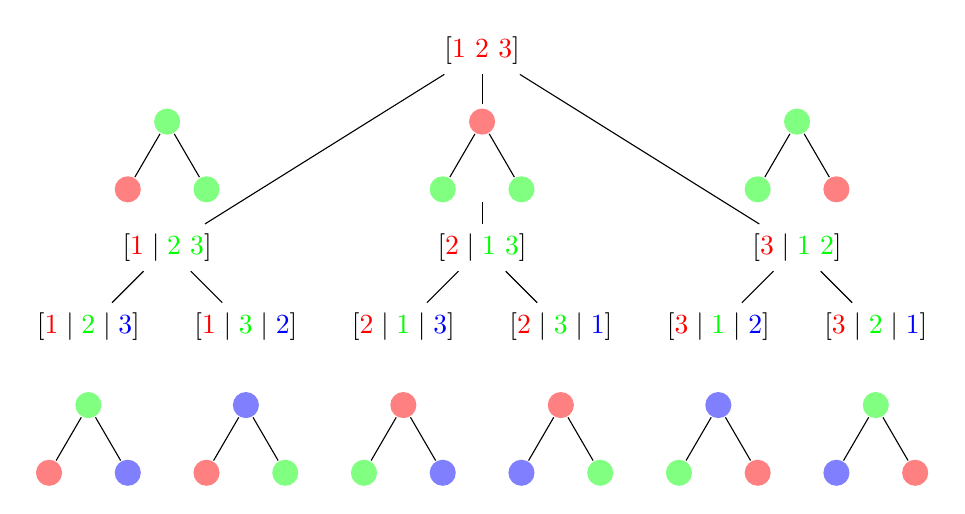
\begin{tikzpicture}
		   \begin{scope}
			   \node (0) at (0, 1.5) {$[{\color{red}1\ 2\ 3}]$};
			   \node (1) at (-4, -1) {$[{\color{red}1} \mid {\color{green}2\ 3}]$};
			   \node (2) at (0, -1) {$[{\color{red}2} \mid {\color{green}1\ 3}]$};
			   \node (3) at (4, -1) {$[{\color{red}3} \mid {\color{green}1\ 2}]$};
			   \node (12) at (-5, -2) {$[{\color{red}1} \mid {\color{green}2} \mid {\color{blue}3}]$};
			   \node (13) at (-3, -2) {$[{\color{red}1} \mid {\color{green}3} \mid {\color{blue}2}]$};
			   \node (21) at (-1, -2) {$[{\color{red}2} \mid {\color{green}1} \mid {\color{blue}3}]$};
			   \node (23) at (1, -2) {$[{\color{red}2} \mid {\color{green}3} \mid {\color{blue}1}]$};
			   \node (31) at (3, -2) {$[{\color{red}3} \mid {\color{green}1} \mid {\color{blue}2}]$};
			   \node (32) at (5, -2) {$[{\color{red}3} \mid {\color{green}2} \mid {\color{blue}1}]$};

			   \node (a1) at (-5.5, -3.86)[pointred] {};
			   \node (a2) at (-5, -3)[pointgreen] {};
			   \node (a3) at (-4.5, -3.86)[pointblue] {};

			   \node (b1) at (-3.5, -3.86)[pointred] {};
			   \node (b2) at (-3, -3)[pointblue] {};
			   \node (b3) at (-2.5, -3.86)[pointgreen] {};

			   \node (c1) at (-1.5, -3.86)[pointgreen] {};
			   \node (c2) at (-1, -3)[pointred] {};
			   \node (c3) at (-0.5, -3.86)[pointblue] {};

			   \node (d1) at (0.5, -3.86)[pointblue] {};
			   \node (d2) at (1, -3)[pointred] {};
			   \node (d3) at (1.5, -3.86)[pointgreen] {};

			   \node (e1) at (2.5, -3.86)[pointgreen] {};
			   \node (e2) at (3, -3)[pointblue] {};
			   \node (e3) at (3.5, -3.86)[pointred] {};

			   \node (f1) at (4.5, -3.86)[pointblue] {};
			   \node (f2) at (5, -3)[pointgreen] {};
			   \node (f3) at (5.5, -3.86)[pointred] {};

			   \node (g1) at (-4.5, -0.26)[pointred] {};
			   \node (g2) at (-4, 0.6)[pointgreen] {};
			   \node (g3) at (-3.5, -0.26)[pointgreen] {};

			   \node (h1) at (-0.5, -0.26)[pointgreen] {};
			   \node (h2) at (0, 0.6)[pointred] {};
			   \node (h3) at (0.5, -0.26)[pointgreen] {};

			   \node (i1) at (4.5, -0.26)[pointred] {};
			   \node (i2) at (4, 0.6)[pointgreen] {};
			   \node (i3) at (3.5, -0.26)[pointgreen] {};

			   \node (dummy1) at (0, 0.7)[opacity=0] {};
			   \node (dummy2) at (0, -0.3)[opacity=0] {};
		   \end{scope}
		   \begin{scope}
			   \path [-] (0) edge (1);
			   \path [-] (0) edge (dummy1);
			   \path [-] (dummy2) edge (2);
			   \path [-] (0) edge (3);
			   \path [-] (1) edge (12);
			   \path [-] (1) edge (13);
			   \path [-] (2) edge (21);
			   \path [-] (2) edge (23);
			   \path [-] (3) edge (31);
			   \path [-] (3) edge (32);

			   \path [-] (a1) edge (a2);
			   \path [-] (a2) edge (a3);

			   \path [-] (b1) edge (b2);
			   \path [-] (b2) edge (b3);

			   \path [-] (c1) edge (c2);
			   \path [-] (c2) edge (c3);

			   \path [-] (d1) edge (d2);
			   \path [-] (d2) edge (d3);

			   \path [-] (e1) edge (e2);
			   \path [-] (e2) edge (e3);

			   \path [-] (f1) edge (f2);
			   \path [-] (f2) edge (f3);

			   \path [-] (g1) edge (g2);
			   \path [-] (g2) edge (g3);

			   \path [-] (h1) edge (h2);
			   \path [-] (h2) edge (h3);

			   \path [-] (i1) edge (i2);
			   \path [-] (i2) edge (i3);
		   \end{scope}
	   \end{tikzpicture}
	   \caption{Stablo pretrage koje generiše sve permutacije skupa čvorova.}
	   \label{img:tree}
   \end{figure}

  Dejstvo grupe $S_n$ na stablo definiše se slično kao za bilo koju drugu
  strukturu. Naredna lema pokazuje da je ovako definisano stablo invarijantno na
  imenovanje čvorova grafa.

  \begin{lemma}
      Za svaki obojen graf $(G, \pi)$ i svako $g \in S_n$ važi
      $\mathcal{T}(G^g, \pi^g) = \mathcal{T}(G, \pi)^g$.
  \end{lemma}

  \begin{proof}
      Dokažimo da za svaki čvor $\nu$ stabla $\mathcal{T}(G, \pi)$ važi da je
      $\nu^g$ čvor stabla $\mathcal{T}(G^g, \pi^g)$. Dokaz izvodimo indukcijom
      po strukturi stabla.
      \begin{itemize}
     	 \item[] \textbf{Baza indukcije} Prazan niz je koren stabla
     		 $\mathcal{T}(G^g, \pi^g)$, pa tvrđenje trivijalno važi.
     	 \item[] \textbf{Induktivni korak} Pretpostavimo da tvrđenje važi za
     		 čvor $\nu$. Neka je $\nu \| w$ dete čvora $\nu$ za neko $w \in
     		 T(G, \pi, \nu)$. Tada je $(\nu \| w)^g = \nu^g \| w^g$, ali kako
     		 važi $w^g \in T(G, \pi, \nu)^g =_{(T3)} T(G^g, \pi^g, \nu^g)$
     		 to je $\nu^g \| w^g$ dete čvora $\nu^g$ u stablu $\mathcal{T}(G^g,
     		 \pi^g)$.
      \end{itemize}
	  Time smo dokazali da je stablo $\mathcal{T}(G, \pi)^g$ podstablo od
	  $\mathcal{T}(G^g, \pi^g)$ ($\mathcal{T}(G, \pi)^g \subseteq
	  \mathcal{T}(G^g, \pi^g)$). Prema prethodno dokazanom važi
	  $\mathcal{T}(G^g, \pi^g)^{g^{-1}} \subseteq \mathcal{T}((G^g)^{g^{-1}},
	  (\pi^g)^{g^{-1}}) = \mathcal{T}(G, \pi)$, pa primenom $g$ na obe strane
	  konačno dobijamo $\mathcal{T}(G^g, \pi^g) \subseteq \mathcal{T}(G,
	  \pi)^g$.
  \end{proof}

  \begin{corrolary}
	  \label{corr:auttree}
      Neka je $\nu$ čvor stabla $\mathcal{T}(G, \pi)$ i neka $\mathcal{T}(G,
      \pi, \nu)$ označava njegovo podstablo sa korenom u $\nu$. Ako je $g
      \in Aut(G, \pi)$, onda je $\nu^g$ čvor stabla $\mathcal{T}(G, \pi)$ i
      važi $\mathcal{T}(G, \pi, \nu^g) = \mathcal{T}(G, \pi, \nu)^g$.
  \end{corrolary}

  \begin{lemma}
	  Neka je $\nu$ čvor stabla $\mathcal{T}(G, \pi)$ i $\pi_\nu = R(G, \pi,
	  \nu)$. Tada je grupa automorfizama obojenog grafa $(G, \pi_\nu)$ jednaka
	  stabilizatoru niza $\nu$ u grupi automorfizama grafa $(G, \pi)$, odnosno
	  $Aut(G, \pi_\nu) = \Sigma_\nu^{Aut(G, \pi)}$.
  \end{lemma}

  \begin{proof}
	  Neka je $g \in Aut(G, \pi_\nu)$. Tada je $\pi_\nu^g = \pi_\nu$, pa za
	  svako $v$ važi $\pi_\nu^g(v) = \pi_\nu(v)$. Na osnovu uslova $(R2)$ za $v
	  \in \nu$ važi $\{v\} = \pi_\nu^{-1}(\pi_\nu(v)) =
	  \pi_\nu^{-1}(\pi_\nu^g(v)) = \pi_\nu^{-1}(\pi_\nu(g^{-1}v)) \ni g^{-1}v$
	  odakle sledi $v^g = v$, odnosno $g$ stabilizuje svako $v \in \nu$.

	  Sa druge strane, neka $g \in Aut(G, \pi)$ stabilizuje $\nu$. Tada po (R3)
	  važi $\pi_\nu^g = R(G, \pi, \nu)^g = R(G^g, \pi^g, \nu^g) = R(G, \pi,
	  \nu) = \pi_\nu$, pa je $g \in Aut(G, \pi_\nu)$.
  \end{proof}

 \section{Invarijanta stabla}

  \begin{definition}
	  \emph{Invarijanta stabla} je preslikavanje $\phi : \mathcal{G} \times \Pi
	  \times V^* \to F$ za neki potpuno uređen skup $F$ koje za sve obojene
	  grafove $(G, \pi)$ i različite čvorove $\nu_1, \nu_2 \in \mathcal{T}(G,
	  \pi)$ ispunjava sledeće uslove:

	  \begin{itemize}
		  \item[(\phi1)] Ako su $\nu_1, \nu_2 \in \mathcal{T}(G, \pi)$ takvi
			  da je $|\nu_1|=|\nu_2|$ i $\phi(G, \pi, \nu_1) < \phi(G,
			  \pi, \nu_2)$, onda za sve $\omega_1 \in \mathcal{T}(G, \pi,
			  \nu_1)$ i $\omega_2 \in \mathcal{T}(G, \pi, \nu_2)$ važi
			  $\phi(G, \pi, \omega_1) < \phi(G, \pi, \omega_2)$
		  \item[(\phi2)] Ako su $\nu_1, \nu_2 \in \mathcal{T}(G, \pi)$ takvi
			  da su $\pi_1 = R(G, \pi, \nu_1)$ i $\pi_2 = R(G, \pi, \nu_2)$
			  diskretna bojenja, onda je $\phi(G, \pi, \nu_1) = \phi(G,
			  \pi, \nu_2) \implies G^{\pi_1} = G^{\pi_2}$
		  \item[(\phi3)] $\phi$ je funkcija invarijantna na imenovanje čvorova
			  grafa
	  \end{itemize}

	  Listovi $\nu_1$ i $\nu_2$ su \emph{ekvivalentni} ako i samo ako $\phi(G,
	  \pi, \nu_1) = \phi(G, \pi, \nu_2)$.
  \end{definition}

  Neformalno, prvi uslov obezbeđuje da ako je vrednost invarijante u čvoru
  $\nu_1$ manja od vrednosti invarijante u čvoru $\nu_2$ istog nivoa, tada to
  važi i za sve parove čvorova njihovih podstabala. Drugi uslov garantuje da su
  grafovi dobijeni transformacijom polaznog grafa primenom bojenja u
  ekvivalentnim listovima jednaki.

  \begin{example}
	  Definišimo $\phi(G, \pi, \nu)$ koristeći pomoćnu funkciju $f$ kao niz
	  vrednosti $(f(G, \pi, [\nu]_0), f(G, \pi, [\nu]_1), \dots, f(G, \pi,
	  [\nu]_{|\nu|}))$, pri čemu u slučaju da je $\nu$ list možemo na taj niz
	  nadovezati i binarnu reprezentaciju grafa permutovanog bojenjem $R(G,
	  \pi, \nu)$. Ovako definisano $\phi$ ispunjava uslove ($\phi$1-2). Ako za
	  pomoćnu funkciju $f$ odaberemo npr. proizvod zbirova stepena čvorova
	  ćelija, dobijamo jednu jednostavnu invarijantu stabla (npr. za bojenje
	  $[2 \mid 1\ 3]$ zbir stepena čvorova prve ćelije je $2$, a druge je $1 +
	  1$, pa je vrednost funkcije $2(1+1)=4$ za ovo bojenje). Vrednosti
	  invarijante stabla iz primera \ref{img:tree} prikazane su na slici
	  \ref{img:invariant}.
  \end{example}

   \begin{figure}[htp]
	   \centering
	   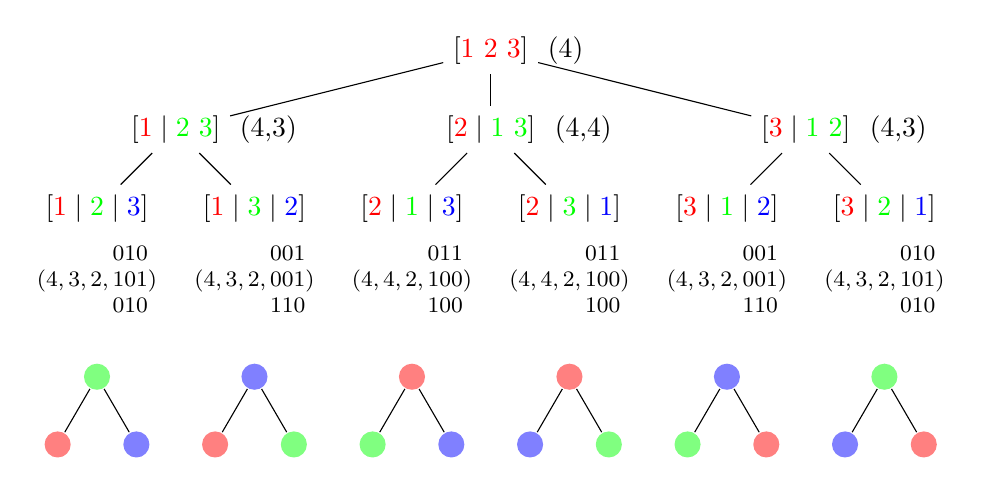
\begin{tikzpicture}
		   \begin{scope}
			   \node (0) at (0, 0) [label=0:{(4)}] {$[{\color{red}1\ 2\ 3}]$};
			   \node (1) at (-4, -1) [label=0:{(4,3)}] {$[{\color{red}1} \mid {\color{green}2\ 3}]$};
			   \node (2) at (0, -1) [label=0:{(4,4)}] {$[{\color{red}2} \mid {\color{green}1\ 3}]$};
			   \node (3) at (4, -1) [label=0:{(4,3)}] {$[{\color{red}3} \mid {\color{green}1\ 2}]$};
			   \node (12) at (-5, -2) [label=270:{\footnotesize $(4,3,2,\begin{matrix}010\\101\\010\end{matrix})$}] {$[{\color{red}1} \mid {\color{green}2} \mid {\color{blue}3}]$};
			   \node (13) at (-3, -2) [label=270:{\footnotesize $(4,3,2,\begin{matrix}001\\001\\110\end{matrix})$}] {$[{\color{red}1} \mid {\color{green}3} \mid {\color{blue}2}]$};
			   \node (21) at (-1, -2) [label=270:{\footnotesize $(4,4,2,\begin{matrix}011\\100\\100\end{matrix})$}] {$[{\color{red}2} \mid {\color{green}1} \mid {\color{blue}3}]$};
			   \node (23) at (1, -2) [label=270:{\footnotesize $(4,4,2,\begin{matrix}011\\100\\100\end{matrix})$}] {$[{\color{red}2} \mid {\color{green}3} \mid {\color{blue}1}]$};
			   \node (31) at (3, -2) [label=270:{\footnotesize $(4,3,2,\begin{matrix}001\\001\\110\end{matrix})$}] {$[{\color{red}3} \mid {\color{green}1} \mid {\color{blue}2}]$};
			   \node (32) at (5, -2) [label=270:{\footnotesize $(4,3,2,\begin{matrix}010\\101\\010\end{matrix})$}] {$[{\color{red}3} \mid {\color{green}2} \mid {\color{blue}1}]$};

			   \node (a1) at (-5.5, -5)[pointred] {};
			   \node (a2) at (-5, -4.14)[pointgreen] {};
			   \node (a3) at (-4.5, -5)[pointblue] {};

			   \node (b1) at (-3.5, -5) [pointred] {};
			   \node (b2) at (-3, -4.14)[pointblue] {};
			   \node (b3) at (-2.5, -5)[pointgreen] {};

			   \node (c1) at (-1.5, -5)[pointgreen] {};
			   \node (c2) at (-1, -4.14)[pointred] {};
			   \node (c3) at (-0.5, -5)[pointblue] {};

			   \node (d1) at (0.5, -5)[pointblue] {};
			   \node (d2) at (1, -4.14)[pointred] {};
			   \node (d3) at (1.5, -5)[pointgreen] {};

			   \node (e1) at (2.5, -5)[pointgreen] {};
			   \node (e2) at (3, -4.14)[pointblue] {};
			   \node (e3) at (3.5, -5)[pointred] {};

			   \node (f1) at (4.5, -5)[pointblue] {};
			   \node (f2) at (5, -4.14)[pointgreen] {};
			   \node (f3) at (5.5, -5)[pointred] {};
		   \end{scope}
		   \begin{scope}
			   \path [-] (0) edge (1);
			   \path [-] (0) edge (2);
			   \path [-] (0) edge (3);
			   \path [-] (1) edge (12);
			   \path [-] (1) edge (13);
			   \path [-] (2) edge (21);
			   \path [-] (2) edge (23);
			   \path [-] (3) edge (31);
			   \path [-] (3) edge (32);

			   \path [-] (a1) edge (a2);
			   \path [-] (a2) edge (a3);

			   \path [-] (b1) edge (b2);
			   \path [-] (b2) edge (b3);

			   \path [-] (c1) edge (c2);
			   \path [-] (c2) edge (c3);

			   \path [-] (d1) edge (d2);
			   \path [-] (d2) edge (d3);

			   \path [-] (e1) edge (e2);
			   \path [-] (e2) edge (e3);

			   \path [-] (f1) edge (f2);
			   \path [-] (f2) edge (f3);
		   \end{scope}
	   \end{tikzpicture}
	   \caption{Invarijanta stabla.}
	   \label{img:invariant}
   \end{figure}


  U nastavku ćemo kroz dve teoreme prikazati značaj ovako definisane
  invarijante stabla. Označimo za proizvoljan čvor stabla $\nu$ njegovo bojenje
  dobijeno funkcijom profinjavanja sa $\pi_\nu = R(G, \pi, \nu)$. 

  \begin{lemma}
	  \label{lemma:autequiv}
	  Neka je $g \in Aut(G, \pi)$ i listovi $\nu_1$ i $\nu_2$ takvi da je
	  $\nu_1^g = \nu_2$. Tada su $\nu_1$ i $\nu_2$ ekvivalentni i $g =
	  \pi_{\nu_2}^{-1}\pi_{\nu_1}$.
  \end{lemma}

  \begin{proof}
	  Na osnovu svojstva ($\phi3$) invarijante stabla i činjenice da je $g$
	  automorfizam sledi $\phi(G, \pi, \nu_1) =_{(\phi_3)} \phi(G^g, \pi^g,
	  \nu_1^g) =_{g \in Aut(G, \pi)} \phi(G, \pi, \nu_1^g) = \phi(G, \pi,
	  \nu_2)$, odnosno $\nu_1$ i $\nu_2$ su ekvivalentni. Dalje, važi
	  $\pi_{\nu_2}^{-1}\pi_{\nu_1} = \pi_{\nu_1^g}^{-1}\pi_{\nu_1} =_{(R3)}
	  (\pi_{\nu_1}^g)^{-1}\pi_{\nu_1} = (\pi_{\nu_1} g^{-1})^{-1} \pi_{\nu_1} = g
	  \pi_{\nu_1}^{-1} \pi_{\nu_1} = g$.
  \end{proof}

  \begin{lemma}
	  Neka su $\alpha$ i $\beta$ diskretna bojenja finija od bojenja $\pi$.
	  Tada je $\pi^\alpha = \pi^\beta$.
  \end{lemma}

  \begin{proof}
	  Dokaz izvodimo nizom pomoćnih tvrđenja.

	  \begin{enumerate}
		  \item $id \leq \pi^\alpha$

			  Neka su $x$ i $y$ proizvoljne vrednosti. Važi $\pi^\alpha(x) <
			  \pi^\alpha(y) \iff \pi(\alpha^{-1}(x)) < \pi(\alpha^{-1}(y))$, pa
			  kako je $\alpha \leq \pi$ sledi $\alpha(\alpha^{-1}(x)) <
			  \alpha(\alpha^{-1}(y))$ odnosno $x < y$. Kontrapozicijom dobijamo
			  i $x \leq y \implies \pi^\alpha(x) \leq \pi^\alpha(y)$.

		  \item $(\pi^\alpha)^{-1}(c) = [n, m]$ za neko $n, m \in \mathbb{N}$
			  gde je $[n, m] = \{k \in \mathbb{N} \mid n \leq k \leq m\}$

			  Za svako $x, y, z $ važi $x \leq y \leq z \implies \pi^\alpha(x)
			  \leq \pi^\alpha(y) \leq \pi^\alpha(z)$, pa ako je $\pi^\alpha(x)
			  = \pi^\alpha(z) = c$, onda je i $\pi^\alpha(y) = c$.

		  \item $\pi^\alpha(n + 1) = \pi^\alpha(n)$ ili $\pi^\alpha(n+1) =
			  \pi^\alpha(n) + 1$

			  Neka je $\pi^\alpha(n+1) \neq \pi^\alpha(n)$. Tada je $n + 1 \geq
			  n \implies \pi^\alpha(n+1) \geq \pi^\alpha(n)$, pa je
			  $\pi^\alpha(n+1) > \pi^\alpha(n)$ jer su po pretpostavci
			  različiti. Pretpostavimo da je $\pi^\alpha(n+1) > \pi^\alpha(n) +
			  1$. Tada postoji $m$ takvo da je $\pi^\alpha(m) = \pi^\alpha(n) +
			  1$, ali iz $\pi^\alpha(n) < \pi^\alpha(m) < \pi^\alpha(n+1)
			  \implies n < m < n + 1$ sledi kontradikcija.

		  \item $|(\pi^\alpha)^{-1}(c)| = |\pi^{-1}(c)|$

			  Važi da je $(\pi^\alpha)^{-1}(c) = \pi^{-1}(c)^\alpha$ odakle je
			  $|(\pi^\alpha)^{-1}(c)| = |\pi^{-1}(c)^\alpha| = |\pi^{-1}(c)|$.

		  \item $(\pi^\alpha)^{-1}(c) = (\pi^\beta)^{-1}(c)$

			  Dokaz izvodimo indukcijom po $c$.

			  \begin{itemize}
				  \item[] \textbf{Baza indukcije} Kako je $1 \leq x$ za sve
					  $x$, onda iz $id \leq \pi^\alpha$ sledi $\pi^\alpha(1)
					  \leq \pi^\alpha(x)$ za sve $x$ pa je $\pi^\alpha(1) = 1$.
					  Dalje, kako je $|(\pi^\alpha)^{-1}(1)| = |\pi^{-1}(1)|$,
					  mora važiti $(\pi^\alpha)^{-1}(1) = [1, |\pi^{-1}(1)|]$.
					  Analogno se pokazuje i za $\beta$.

				  \item[] \textbf{Induktivni korak} Neka je po induktivnoj
					  pretpostavci $(\pi^\alpha)^{-1}(c) = (\pi^\beta)^{-1}(c)
					  = [n, m]$. Tada je $\pi^\alpha(m+1) \neq \pi^\alpha(m)$,
					  pa je $\pi^\alpha(m+1) = \pi^\alpha(m) + 1$ i $m+1$ je
					  najmanje u $(\pi^\alpha)^{-1}(c+1)$. Odatle važi
					  $(\pi^\alpha)^{-1}(c+1) = [m + 1, m + |\pi^{-1}(c+1)|]$.
					  Analogno se pokazuje i za $\beta$.
			  \end{itemize}
	  \end{enumerate}
  \end{proof}

  \begin{theorem}
	  \label{thm:aut}
	  Za svaki list $\nu$ važi $Aut(G, \pi) = \{\pi_{\omega}^{-1}\pi_{\nu}
	  \mid \text{$\nu$ i $\omega$ su ekvivalentni} \}$.
  \end{theorem}
  
  \begin{proof}
	  Neka je $g \in Aut(G, \pi)$. Tada je po posledici \ref{corr:auttree}
	  $\nu^g$ list stabla $\mathcal{T}(G, \pi)$. Po prethodno dokazanoj lemi
	  \ref{lemma:autequiv} su $\nu$ i $\nu^g$ ekvivalentni i $g =
	  \pi_{\nu^g}^{-1}\pi_\nu$ što je element skupa sa desne strane jednakosti.
	  Sa druge strane, ako su $\nu$ i $\omega$ ekvivalentni, onda je
	  $G^{\pi_\nu} = G^{\pi_\omega}$, pa je $\pi_\omega^{-1}\pi_\nu \in Aut(G,
	  \pi)$.
  \end{proof}

	Prethodna teorema pokazuje da je otkrivanjem svih listova ekvivalentnih
	jednom listu moguće odrediti grupu automorfizama datog grafa. Naravno,
	ovakav način određivanja grupe automorfizama nije veoma efikasan pošto se
	grupa generiše član po član. Ovo se može poboljšati odsecanjem pretrage o
	čemu će biti reči u narednom odeljku.
	
	\begin{example}
		Posmatrajmo prvi list $\zeta$ stabla sa slike \ref{img:invariant}. Na
		osnovu prethodne teoreme je moguće odrediti skup svih automorfizama
		grafa.  Kako je list $\zeta$ ekvivalentan samom sebi, $id \in
		Aut(G, \pi)$.  Kako je ekvivalentan poslednjem listu $\nu$ stabla,
		$\pi_\nu^{-1}\pi_\zeta = \begin{pmatrix}1 & 2 & 3\\3 & 2 &
			1\end{pmatrix}^{-1}\begin{pmatrix}1 & 2 & 3\\1 & 2 &
		3\end{pmatrix}=(1\ 3) \in Aut(G, \pi)$. Ne postoje drugi automorfizmi
		jer ne postoje drugi listovi ekvivalentni prvom listu stabla, pa je
		$Aut(G, \pi) = \{id, (1\ 3)\}$.
	\end{example}

  \begin{definition}
	  Neka je $\nu^*$ list stabla $\mathcal{T}(G, \pi)$ u kom invarijanta
	  $\phi(G, \pi, \nu)$ dostiže maksimum. \emph{Kanonska forma određena
	  invarijantom stabla} obojenog grafa $(G, \pi)$ je funkcija
	  $\mathcal{C}(G, \pi) = (G, \pi)^{\pi_{\nu^*}}$.
  \end{definition}

  Primetimo da zbog uslova $(\phi2)$ definicija ne zavisi od izbora lista
  $\nu^*$. Naredna teorema opravdava naziv i oznaku funkcije.

  \begin{theorem}
	  Funkcija $\mathcal{C}(G, \pi)$ je kanonska forma.
  \end{theorem}

  \begin{proof}
		Dokazujemo da ovako definisana funkcija ispunjava uslove kanonske forme za
		svaki obojen graf $(G, \pi)$.
	  \begin{itemize}
		  \item [($\mathcal{C}1$)] Kako je $\mathcal{C}(G, \pi) = (G,
			  \pi)^{\pi_{\nu^*}}$ to je $\mathcal{C}(G, \pi) \cong (G, \pi)$ za
			  izomorfizam $\pi_{\nu^*}$.
		  \item [($\mathcal{C}2$)] Za svako $g \in S_n$ i svako $\nu \in
			  \mathcal{T}(G, \pi)$ važi $\nu^g \in \mathcal{T}(G, \pi)^g =
			  \mathcal{T}(G^g, \pi^g)$ kao i $\phi(G^g, \pi^g, \nu^g) = \phi(G,
			  \pi, \nu)$, pa je $\nu^*^g$ list u kom invarijanta stabla
			  $\mathcal{T}(G^g, \pi^g)$ dostiže maksimalnu vrednost.  Odatle
			  sledi $\mathcal{C}(G^g, \pi^g) = (G^g, \pi^g)^{R(G^g, \pi^g,
			  \nu^*^g)} = (G^g, \pi^g)^{\pi_{v^*}^g} = (G, \pi)^{\pi_{v^*}} =
			  \mathcal{C}(G, \pi)$ pa je $\mathcal{C}$ funkcija invarijantna na
			  imenovanje čvorova.
	  \end{itemize}
  \end{proof}

	\begin{example}
		Posmatrajmo stablo sa slike \ref{img:invariant}. Na osnovu prethodne
		teoreme je moguće odrediti kanonsku formu grafa. U pitanju je graf koji
		se dobija bilo kojom od permutacija $g_1 = [2 \mid 1 \mid 3]$ tj. $g_1 : \begin{pmatrix} 1 & 2 & 3 \\
		2 & 1 & 3\end{pmatrix}$ ili $g_2 = [2 \mid 3 \mid 1]$ tj. $g_2 : \begin{pmatrix} 1 & 2 & 3 \\ 3 &
		1 & 2 \end{pmatrix}$ jer su to permutacije sa najvećom invarijantom u
		stablu.
	\end{example}

 \section{Odsecanje pretrage}

  Stablo pretrage može biti veoma veliko, pa pretraga kompletnog stabla nije
  poželjna. To možemo rešiti uvođenjem tri različite operacije odsecanja.
  \begin{itemize}
	  \item Neka su $\nu_1$ i $\nu_2$ različiti čvorovi stabla $\mathcal{T}(G,
		  \pi)$ takvi da je $|\nu_1|=|\nu_2|$ i $\phi(G, \pi, \nu_1) >
		  \phi(G, \pi, \nu_2)$. Operacija $P_A(\nu_1, \nu_2)$ podrazumeva
		  odsecanje podstabla $\mathcal{T}(G, \pi, \nu_2)$.
	  \item Neka su $\nu_1$ i $\nu_2$ različiti čvorovi stabla $\mathcal{T}(G,
		  \pi)$ takvi da je $|\nu_1|=|\nu_2|$ i $\phi(G, \pi, \nu_1) \neq
		  \phi(G, \pi, \nu_2)$. Operacija $P_B(\nu_1, \nu_2)$ podrazumeva
		  odsecanje podstabla $\mathcal{T}(G, \pi, \nu_2)$.
	  \item Neka su $\nu_1$ i $\nu_2$ različiti čvorovi stabla $\mathcal{T}(G,
		  \pi)$ takvi da je $\nu_1 < \nu_2$ i $\nu_1^g=\nu_2$ za neko $g \in
		  Aut(G, \pi)$. Operacija $P_C(\nu_1, g)$ podrazumeva odsecanje
		  podstabla $\mathcal{T}(G, \pi, \nu_2)$.
  \end{itemize}

  Operacije $P_A$ i $P_C$ su definisane tako da proizvoljna primena ovih
  operacija ne uklanja mogućnost određivanja kanonske forme u stablu. Slično,
  proizvoljna primena operacija $P_B$ i $P_C$ ne uklanja mogućnost određivanja
  grupe automorfizama grafa. Naredna teorema opravdava uvođenje ovih operacija
  i pokazuje da one ne narušavaju rezultate teorema o određivanju grupe
  automorfizama i kanonske forme.

  \begin{theorem}
	  Neka je $(G, \pi)$ obojen graf.
	  \begin{enumerate}
		  \item Neka je nad stablom $\mathcal{T}(G, \pi)$ izvršen proizvoljan
			  niz operacija $P_A$ i $P_C$. Tada u dobijenom stablu postoji bar
			  jedan list $\nu$ takav da je $\phi(G, \pi, \nu) = \phi(G, \pi,
			  \nu^*)$.
		  \item Neka je $\nu_0$ list stabla $\mathcal{T}(G, \pi)$ i neka je nad
			  stablom izvršen proizvoljan niz operacija $P_B(\nu_1, \nu_2)$ i
			  $P_C$ gde je $\phi(G, \pi, \nu_2) \neq \phi(G, \pi,
			  [\nu_0]_{s})$ za sve $0 \leq s \leq |\nu_0|$ i neka su $g_1,
			  \dots, g_k$ svi automorfizmi korišćeni u izvršenim operacijama
			  $P_C$.  Tada je grupa automorfizama $Aut(G, \pi)$ generisana
			  skupom $\{g_1, \dots, g_k\} \cup \{g \in Aut(G, \pi) \mid \nu_0^g
			  \text{ nije uklonjen}\}$.
	  \end{enumerate}
  \end{theorem}

  \begin{proof}
	  Dokažimo za početak nekoliko pomoćnih tvrđenja.

	  Nijedna operacija $P_A$ ne uklanja listove u kojima je vrednost
	  invarijante maksimalna. Pretpostavimo suprotno. Neka je $\nu_1$ list u
	  kom invarijanta stabla dostiže maksimum i neka je $\nu'_1$ predak od
	  $\nu_1$. Operacija $P_A(\nu'_2, \nu'_1)$ uklanja $\nu'_1$ ako je $\phi(G,
	  \pi, \nu'_1) < \phi(G, \pi, \nu'_2)$, pa po svojstvu $(\phi1)$ za
	  proizvoljan list $\nu_2$ u $\mathcal{T}(G, \pi, \nu'_2)$ važi $\phi(G,
	  \pi, \nu_1) < \phi(G, \pi, \nu_2)$, što je u kontradikciji sa
	  pretpostavkom da je vrednost invarijante maksimalna u $\nu_1$.

	  Nijedna operacija $P_B$ ne uklanja nijedan list $\nu$ ekvivalentan listu
	  $\nu_0$ (iz drugog dela teoreme). Iz pretpostavke teoreme nijedna
	  operacija $P_B(\nu_1, \nu_2)$ ne uklanja čvor $\nu_2$ takav da je
	  $\phi(G, \pi, [\nu_0]_{|\nu_2|}) = \phi(G, \pi, \nu_2)$, pa samim tim ne
	  uklanja nijedan čvor $[\nu]_{s}$ za $0 \leq s \leq |\nu|$.

	  Nijedna operacija $P_C$ ne uklanja leksikografski najmanji među
	  ekvivalentnim listovima. Štaviše, nijedna operacija $P_C$ ne uklanja
	  leksikografski najmanji čvor iz $\Omega_\nu^{\langle g_1, \dots, g_k
	  \rangle}$ za bilo koje $\nu$. Neka je bez umanjenja opštosti $\nu$
	  leksikografski najmanji list u svojoj orbiti. Operacija $P_C(\omega, g)$
	  uklanja čvor $\omega^g$ ako je $\omega < \omega^g$, pa je
	  $[\nu]_{|\omega|} \neq \omega^g$ pošto je ili $[\nu]_{|\omega|} < \omega$
	  ili su $\omega$ i $[\nu]_{|\omega|}$ iz različitih orbita.
	  \begin{enumerate}
		  \item Na osnovu dokazanih svojstava operacija $P_A$ i $P_C$ iz stabla
			  se ne uklanja leksikografski najmanji list $\nu$ ekvivalentan
			  listu $\nu^*$.
		  \item Ako je $g \in Aut(G, \pi)$, onda na osnovu dokazanih svojstava
			  operacija $P_B$ i $P_C$ važi da iz stabla nije uklonjen
			  leksikografski najmanji list oblika $\nu_0^{hg}$ za neko $h \in \langle
			  g_1, \dots, g_k \rangle$, izborom $\omega =
			  \nu_0^g$. Odatle sledi da je $hg \in \langle \{g_1, \dots,
			  g_k\} \cup \{g \in Aut(G, \pi) \mid \nu_0^g \text{ nije
			  uklonjen}\} \rangle$, pa je i $g$ element generisane
			  grupe.
	  \end{enumerate}
  \end{proof}

  \begin{example}
	  Prilikom obilaska stabla sa slike \ref{img:invariant} moguće je izvršiti
	  odsecanje nekih delova stabla na osnovu automorfizma $(1\ 3)$ (ukoliko je
	  on poznat unapred).  Rezultujuće stablo je dato na slici \ref{img:prune}.
	  Čvor $(2, 3)$ moguće je odseći na osnovu čvora $(2, 1)$. Čvor $(3)$
	  moguće je odseći na osnovu čvora $(1)$.
  \end{example}

   \begin{figure}[htp]
	   \centering
	   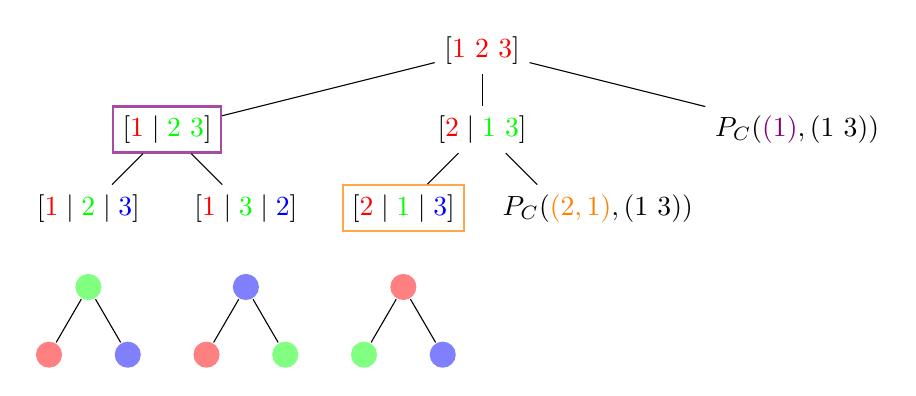
\begin{tikzpicture}
		   \begin{scope}
			   \node (0) at (0, 0)  {$[{\color{red}1\ 2\ 3}]$};
			   \node (1) at (-4, -1) [rectangle, draw=violet!70, thick] {$[{\color{red}1} \mid {\color{green}2\ 3}]$};
			   \node (2) at (0, -1)  {$[{\color{red}2} \mid {\color{green}1\ 3}]$};
			   \node (3) at (4, -1) [] {$P_C({\color{violet}(1)}, (1\ 3))$};
			   \node (12) at (-5, -2)  {$[{\color{red}1} \mid {\color{green}2} \mid {\color{blue}3}]$};
			   \node (13) at (-3, -2)  {$[{\color{red}1} \mid {\color{green}3} \mid {\color{blue}2}]$};
			   \node (21) at (-1, -2) [rectangle,draw=orange!70,thick] {$[{\color{red}2} \mid {\color{green}1} \mid {\color{blue}3}]$};
			   \node (23) at (1, -2) [] {$\ \ \ \ \ \ \ \ P_C({\color{orange}(2,1)}, (1\ 3))$};

			   \node (a1) at (-5.5, -3.86)[pointred] {};
			   \node (a2) at (-5, -3)[pointgreen] {};
			   \node (a3) at (-4.5, -3.86)[pointblue] {};

			   \node (b1) at (-3.5, -3.86)[pointred] {};
			   \node (b2) at (-3, -3)[pointblue] {};
			   \node (b3) at (-2.5, -3.86)[pointgreen] {};

			   \node (c1) at (-1.5, -3.86)[pointgreen] {};
			   \node (c2) at (-1, -3)[pointred] {};
			   \node (c3) at (-0.5, -3.86)[pointblue] {};
		   \end{scope}
		   \begin{scope}
			   \path [-] (0) edge (1);
			   \path [-] (0) edge (2);
			   \path [-] (0) edge (3);
			   \path [-] (1) edge (12);
			   \path [-] (1) edge (13);
			   \path [-] (2) edge (21);
			   \path [-] (2) edge (23);

			   \path [-] (a1) edge (a2);
			   \path [-] (a2) edge (a3);

			   \path [-] (b1) edge (b2);
			   \path [-] (b2) edge (b3);

			   \path [-] (c1) edge (c2);
			   \path [-] (c2) edge (c3);
		   \end{scope}
	   \end{tikzpicture}
	   \caption{Odsecanje stabla na osnovu automorfizama.}
	   \label{img:prune}
   \end{figure}


% ------------------------------------------------------------------------------
\chapter{Realizacija algoritma}
% ------------------------------------------------------------------------------

 U ovoj glavi konkretizovani su parametri opšteg algoritma.  Uvedeni su pojmovi
 \emph{ekvitabilnog bojenja} i \emph{količničkog grafa} ključni za određivanje
 funkcije profinjavanja i invarijante stabla i prikazani su efikasni postupci
 za njihovo izračunavanje.  Prikazane su strukture podataka za reprezentaciju
 objekata uvedenih u prethodnoj glavi i opisan je kompletan algoritam pretrage
 za određivanje kanonske forme. Na kraju, uveden je pojam \emph{invarijante
 grafa} koji indukuje klasu moćnijih funkcija profinjavanja.

 \section{Reprezentacija podataka}

  \subsection{Bojenje}

   Bojenje $\pi \in \Pi_n$ predstavljeno je permutacijom $p$ i nizom $cells$.
   Permutacija $p$ predstavlja niz koji se dobija nadovezivanjem ćelija
   $\pi^{-1}(1), \dots, \pi^{-1}(k)$ redom, gde je $k$ broj boja i pri čemu su
   elementi jedne ćelije uređeni rastuće. Na primer, bojenje $\pi = [2\ 6 \mid
   4\ 3\ 5 \mid 1]$ predstavljeno je permutacijom $p : \begin{pmatrix} 1 & 2 &
   3 & 4 & 5 & 6\\ 2 & 6 & 3 & 4 & 5 & 1 \end{pmatrix}$ koja se dobija kada se
   poređaju rastuće elementi druge ćelije. Primetimo da u slučaju diskretnog
   bojenja $\pi$ važi $p = \pi^{-1}$.

   Niz $cells$ dužine $n$ upotpunjava permutaciju $p$ podacima o granicama
   ćelija bojenja $\pi$. Ako pozicija $u$ predstavlja početak nove ćelije, tada
   je $cells_u$ takvo da ta ćelija obuhvata tačno pozicije $[u, cells_u)$
   permutacije $p$, a u suprotnom je $cells_u = -1$. Na istom primeru, počeci
   novih ćelija nalaze se na pozicijama 1, 3 i 6, pa je $cells_1 = 3$, $cells_3
   = 6$ i $cells_6 = 7$, dok su vrednosti na ostalim pozicijama -1, odnosno
   $cells = (3, -1, 6, -1, -1, 7)$ jer prva ćelija obuhvata elemente na
   pozicijama $[1,3)$, druga $[3,6)$, a treća $[6,7)$.
   
   Jedna od ključnih operacija nad bojenjem je profinjavanje jedne ćelije. Neka
   je $\pi^{-1}(c)$ jedna ćelija bojenja $\pi$ i neka je svakom čvoru $v$ te
   ćelije dodeljena proizvoljna vrednost $t_v$. Profinjavanje ćelije
   podrazumeva formiranje bojenja $\pi' \leq \pi$ takvog da za $u$ i $v$ iz
   $\pi^{-1}(c)$ važi $\pi'(u) < \pi'(v) \iff t_u < t_v$, dok za sve ostale
   parove $u$ i $v$ važi $\pi'(u) = \pi'(v) \iff \pi(u) = \pi(v)$.

  \begin{algorithm}[H]
	  \caption{Profinjavanje ćelije}
	  \textbf{Ulaz}
		  Obojen graf $(G, \pi)$,
		  boja ćelije koju treba profiniti $c$,\\
		  proizvoljan niz vrednosti $t$\\
	  \textbf{Izlaz}
	  	  Profinjeno bojenje $\pi'$,
		  niz ćelija dobijenih profinjavanjem $C_1, \dots, C_k$,\\
		  indeks prve ćelije među $C_1, \dots, C_k$ sa najvećim brojem elemenata $s$
	  \begin{algorithmic}[1]
		  \Procedure{Refine\_cell}{$G, \pi, c, t$}
		  \State{$\pi' \gets \pi$}
		  \State{$k \gets 1$}
		  \For{$t' \in $ sorted($\{t_v \mid v \in \pi^{-1}(c)\}$)}
			\State{$C_k \gets \{v \in \pi^{-1}(c) \mid t_v = t'\}$}
			\State{$\pi'(v) \gets c + k - 1$ za sve $v \in C_k$}
			\State{$k \gets k + 1$}
	      \EndFor
		  \State{$\pi'(v) \gets \pi(v) + k - 1$ za sve $v$ takve da $\pi(v) > c$ }
		  \State{$s \gets $ indeks prvog skupa među $C_{i, 1 \leq i \leq k}$ sa najvećim brojem elemenata}
		  \State\Return{$\pi', C_1, \dots, C_k, s$}
		  \EndProcedure
	  \end{algorithmic}
  \end{algorithm}

  Opisana reprezentacija bojenja je korisna zato što omogućava da se ovaj
  algoritam implementira tako da mu složenost bude $O(|C| \log |C|)$ gde je $C
  = \pi^{-1}(c)$, pri čemu dominira složenost sortiranja čvorova na osnovu
  vrednosti $t_v$.

  \subsection{Graf}

   Pošto se graf ne menja tokom izvršavanja samog algoritma, moguće je čuvati
   više različitih reprezentacija grafa. Ovde ćemo istaći one delove
   reprezentacije koji su neophodni za dalju diskusiju.

   Obojen graf je predstavljen bojenjem $\pi$ i matricom povezanosti $\psi$.
   Zapazimo sledeća svojstva matrice povezantosti:
   \begin{itemize}
	   \item[$(\psi1)$] $\psi(G, u, v) = \psi(G, v, u)$
	   \item[$(\psi2)$] $\psi(G^g, u^g, v^g) = \psi(G, v, u)$ za proizvoljno $g \in S_n$
   \end{itemize}
   Prvo svojstvo je simetričnost matrice povezanosti koja proizilazi iz
   činjenice da je u neusmerenom grafu $(u, v) \in E$ akko $(v, u) \in E$.
   Drugo svojstvo govori da je matrica povezanosti funkcija invarijantna na
   imenovanje čvorova. Ovo svojstvo će biti značajno u definicijama i dokazima
   koji slede u ovom poglavlju. Invarijantnost važi zato što je $(u, v)$ grana
   grafa $G$ akko je $(u, v)^g = (u^g, v^g)$ grana grafa $G^g$.

 \section{Funkcija odabira ciljne ćelije}

 Postoji više strategija za realizaciju funkcije odabira ciljne ćelije. Ovde
 ćemo predstaviti dve takve strategije.

 Jedna mogućnost je odabir neke (konkretno prve) višečlane ćelije bojenja
 najmanje veličine. Obrazloženje za ovakav izbor je da manje ćelije imaju veću
 šansu da sadrže mali broj orbita (ili čak jednu) \cite{McKay} i da je samim
 tim očekivani faktor grananja manji.

 Druga mogućnost, koja se ispostavila kao bolja u većini slučajeva je odabir
 prve višečlane ćelije bez obzira na njenu veličinu \cite{McKay}. U daljem radu
 pretpostavljamo postojanje procedure \texttt{Target\_cell($\pi$)} koja
 implementira ovu strategiju.

 \section{Funkcija profinjavanja}

  Definiciju funkcije profinjavanja ćemo podeliti na dve komponente. Prva
  komponenta je transformacija koja određuje kako se vrši prelaz sa čvora $\nu$
  na čvor $\nu \| w$ u stablu, odnosno kako se izbor čvora $w$ odražava na
  bojenje.

  \begin{definition}
	  Preslikavanje $I : \Pi \times V \to \Pi$ definisano sa
	  $$
	  I(\pi, v)(w) =
	  \begin{cases}
		  \pi(w), & \quad \text{ako je } \pi(w) < \pi(v) \text{ ili } w = v \\
		  \pi(w) + 1, & \quad \text{inače}\\
	  \end{cases}
	  $$
	  naziva se \emph{funkcija individualizacije}.
  \end{definition}

  Uloga funkcije individualizacije je da od zadatog bojenja formira novo,
  finije bojenje koje se od polaznog razlikuje samo u tome što je odabrani čvor
  izdvojen u zasebnu ćeliju. Ovo će obezbediti ispunjenost uslova (R2) funkcije
  profinjavanja.

  \begin{example}
	  Neka je $\pi = [1\ 3 \mid 2\ 4\ 5]$. Tada je $I(\pi, 4) = [1\ 3 \mid 4
	  \mid 2\ 5]$.
  \end{example}

  Naredno tvrđenje ističe tri važna svojstva funkcije individualizacije.
  Štaviše, za funkciju $I$ moguće bi bilo odabrati bilo koje preslikavanje koje
  ispunjava ta svojstva, ali nam je cilj da individualizaciju razdvojimo od
  ostatka definicije funkcije profinjavanja, pa zbog toga nećemo razmatrati
  druga preslikavanja.
  
  \begin{lemma}
	  Funkcija individualizacije $I$ ispunjava naredne uslove:
	  \begin{itemize}
		  \item[(I1)] Za svako bojenje $\pi$ i čvor $u$ važi $I(\pi, u) \leq \pi$.
		  \item[(I2)] $\{u\}$ je ćelija bojenja $I(\pi, u)$.
		  \item[(I3)] $I$ je transformacija invarijantna na imenovanje čvorova.
	  \end{itemize}
  \end{lemma}
  
  \begin{proof}
	  Dokažimo redom tražena svojstva.
  \begin{itemize}
  \item[(I1)] Neka je $\pi(v) < \pi(w)$. Tada nije istovremeno $I(\pi,
	  u)(v) = \pi(v) + 1$ i $I(\pi, u)(w) = \pi(w)$ jer to povlači da je
	  $\pi(v) \geq \pi(u)$ i $\pi(w) \leq \pi(u)$, odnosno da je $\pi(w) \leq
	  \pi(v)$ što je kontradikcija. U svim ostalim slučajevima iz pretpostavke
	  sledi $I(\pi, u)(v) < I(\pi, u)(w)$.

  \item[(I2)] Ako je $\pi(w) = \pi(v)$ i $w \neq v$ onda je $I(\pi, v)(w) = I(\pi,
	  v)(v) + 1$, a kako je $I(\pi, v) \leq \pi$ onda je $\pi(v) \neq \pi(w)
	  \iff I(\pi, v)(v) \neq I(\pi, v)(w)$ pa je $I(\pi, v)(v) \neq I(\pi,
	  v)(w)$ za sve $w \neq v$.

  \item[(I3)] Neka je $g \in S_n$ proizvoljno. Tada je $I(\pi^g, v^g)(w^g) =
	  \pi(w) \iff I(\pi^g, v^g)(w^g) = \pi^g(w^g) \iff \pi^g(w^g) < \pi^g(v^g)
	  \lor w^g = v^g \iff \pi(w) < \pi(v) \lor w = v \iff I(\pi, v)(w) =
	  \pi(w)$. Slično je i $I(\pi^g, v^g)(w^g) = \pi(w) + 1 \iff I(\pi, v)(w) =
	  \pi(w) + 1$, odnosno $I(\pi^g, v^g)(w^g) = I(\pi, v)(w) = I(\pi,
	  v)^g(w^g)$.
  \end{itemize}
  \end{proof}

	Druga komponenta definicije funkcije profinjavanja je transformacija koja
	se vrši nad bojenjem dobijenim individualizacijom. Cilj ove transformacije
	je da što više profini bojenje kako bi stepen grananja prilikom pretrage
	bio što manji.  Idealna transformacija je takva da ćelije rezultujućeg
	bojenja odgovaraju orbitama čvorova u grupi automorfizama početnog bojenja.
  
  \begin{lemma}
	  Neka je $F : \mathcal{G} \times \Pi \times V^* \to \Pi$ transformacija
	  invarijantna na imenovanje čvorova takva da je $F(G, \pi, \nu) \leq \pi$.
	  Tada je preslikavanje definisano sa
	  \begin{align*}
		  &R(G, \pi, ()) = F(G, \pi, ()) \\
		  &R(G, \pi, \nu \| w) = F(G, I(R(G, \pi, \nu), w), \nu \| w)
	  \end{align}
	  funkcija profinjavanja.
  \end{lemma}

  \begin{proof}
	  Dokažimo indukcijom da ovako definisana funkcija $R$ ispunjava
	  uslove funkcije profinjavanja.
	  \begin{itemize}
		  \item[] \textbf{Baza indukcije} 
			  \begin{itemize}
				  \item[(R1)] $R(G, \pi, ()) = F(G, \pi, ()) \leq \pi$
				  \item[(R2)] Tvrđenje trivijalno važi zato što je $()$ prazan niz
				  \item[(R3)] Za svako $g \in S_n$ važi $R(G^g, \pi^g, ()^g) = F(G^g,
					  \pi^g, ()^g) = F(G, \pi, ())^g = R(G, \pi, ())^g$
			  \end{itemize}
		  \item[] \textbf{Induktivni korak} Pretpostavimo da tvrđenje važi za $\nu$.
			  \begin{itemize}
				  \item[(R1)] \phantom{}
					  \begin{aligned}[t]
						  $R(G, \pi, \nu \| w) &= F(G, I(R(G, \pi, \nu), w), \nu
						  \| w) \\
						  &\leq I(R(G, \pi, \nu), w) \\
						  &\leq R(G, \pi, \nu) \\
						  &\leq \pi$
					  \end{aligned}
				  \item[(R2)] $R(G, \pi, \nu \| w) \leq I(R(G, \pi, \nu), w)$
					  pa je ${w}$ ćelija bojenja $R(G, \pi, \nu \| w)$. Ako je
					  $v \in \nu$, onda je ${v}$ ćelija $R(G, \pi, \nu)$, pa je
					  ćelija i bojenja $R(G, \pi, \nu \| w)$ jer je $R(G, \pi,
					  \nu \| w) \leq R(G, \pi, \nu)$.
				  \item[(R3)] Za svako $g \in S_n$ važi \\
					  \begin{aligned}[t]
						  $R(G^g, \pi^g, (\nu \| w)^g) &= F(G^g, I(R(G^g, \pi^g,
						  \nu^g), w^g), (\nu \| w)^g) \\ &= F(G^g, I(R(G, \pi,
						  \nu)^g, w^g), (\nu \| w)^g) \\ &= F(G^g, I(R(G, \pi,
						  \nu), w)^g, (\nu \| w)^g) \\ &= F(G, I(R(G, \pi, \nu),
						  w), (\nu \| w))^g \\ &= R(G, \pi, \nu \| w)^g$
					  \end{aligned}
			  \end{itemize}
	  \end{itemize}
  \end{proof}

  Sada umesto funkcije profinjavanja $R$ kao parametar algoritma posmatramo
  funkciju $F$. Kako bi stablo pretrage bilo što manje, i samim tim pretraga
  efikasnija, ključno je odabrati što moćniju funkciju. U svrhu odabira
  konkretne funkcije $F$ uvodimo pojam \emph{ekvitabilnog bojenja}.

  \begin{definition}
	  Označimo sa $\widetilde{\psi}(G, u, W) = \sum_{w \in W} \psi(G, u, w)$ broj grana
	  grafa $G$ koje povezuju čvor $u$ i skup čvorova $W$.  Particija $\sim$
	  skupa čvorova $V$ je \emph{ekvitabilna} ako za svaki par čvorova $u$ i
	  $v$ takvih da je $u \sim v$ i svaku klasu $C$ particije $\sim$ važi
	  $\widetilde{\psi}(G, u, C) = \widetilde{\psi}(G, v, C)$.  Bojenje $\pi$ je \emph{ekvitabilno} ako
	  je particija $\sim_\pi$ ekvitabilna.
  \end{definition}

  \begin{example}
	  Na slici \ref{img:equitable} su prikazana dva bojenja istog grafa. Levo
	  bojenje je ekvitabilno zato što je svaki zeleni čvor povezan sa tačno dva
	  crna, a svaki crni čvor sa tačno jednim zelenim i tačno jednim crnim.
	  Desno bojenje nije ekvitabilno zato što postoje zeleni čvorovi sa
	  različitim brojem zelenih suseda (levi zeleni čvor nije povezan ni sa
	  jednim zelenim, dok su preostala dva zelena čvora međusobno povezana).
  \end{example}

   \begin{figure}[htp]
	   \centering
	   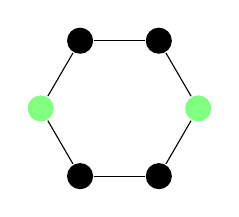
\begin{tikzpicture}
		   \begin{scope}
			   \node (0) at (1, 0)[pointgreen] {};
			   \node (1) at (0.5, 0.86)[point] {};
			   \node (2) at (-0.5, 0.86)[point] {};
			   \node (3) at (-1, 0)[pointgreen] {};
			   \node (4) at (-0.5, -0.86)[point] {};
			   \node (5) at (0.5, -0.86)[point] {};
		   \end{scope}
		   \begin{scope}
			   \path [-] (0) edge (1);
			   \path [-] (1) edge (2);
			   \path [-] (2) edge (3);
			   \path [-] (3) edge (4);
			   \path [-] (4) edge (5);
			   \path [-] (5) edge (0);
		   \end{scope}
	   \end{tikzpicture}
	   \hspace{20pt}
	   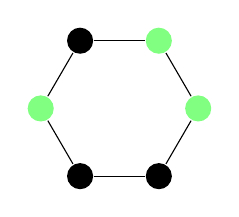
\begin{tikzpicture}
		   \begin{scope}
			   \node (0) at (1, 0)[pointgreen] {};
			   \node (1) at (0.5, 0.86)[pointgreen] {};
			   \node (2) at (-0.5, 0.86)[point] {};
			   \node (3) at (-1, 0)[pointgreen] {};
			   \node (4) at (-0.5, -0.86)[point] {};
			   \node (5) at (0.5, -0.86)[point] {};
		   \end{scope}
		   \begin{scope}
			   \path [-] (0) edge (1);
			   \path [-] (1) edge (2);
			   \path [-] (2) edge (3);
			   \path [-] (3) edge (4);
			   \path [-] (4) edge (5);
			   \path [-] (5) edge (0);
		   \end{scope}
	   \end{tikzpicture}
	   \caption{Primer ekvitabilnog (levo) i neekvitabilnog (desno) bojenja.}
	   \label{img:equitable}
   \end{figure}

  \begin{lemma}
	  \label{lemma:coarsesteq}
	  Za proizvoljno bojenje $\pi$ grafa $G$ postoji jedinstvena najgrublja
	  particija $\sim_\gamma$ koja je ekvitabilna i finija od $\sim_\pi$.
  \end{lemma}

  \begin{proof}
	  Očigledno postoji bar jedna ekvitabilna particija finija od $\sim_\pi$;
	  diskretna particija ispunjava te uslove.  Neka su $\sim_\alpha$ i
	  $\sim_\beta$ dve takve particije. Pokažimo da je particija
	  ${\sim_\alpha}, {\sim_\beta} \leq {\sim_{\alpha \lor \beta}} \leq
	  {\sim_\pi}$ ekvitabilna.

	  Neka je $u \sim_\alpha v$ i neka je $C$ proizvoljna klasa iz
	  $\sim_{\alpha \lor \beta}$. Kako je $\sim_\alpha$ finije od $\sim_{\alpha
	  \lor \beta}$, to je $C = \bigcup_{i=1}^n A_i$ za neke klase $A_1, \dots,
	  A_n$ particije $\sim_\alpha$, pa je $\widetilde{\psi}(G, u, C) =
	  \sum_{i=1}^n \widetilde{\psi}(G, u, A_i)$. Kako je $\alpha$ ekvitabilno,
	  to je dalje jednako $\sum_{i=1}^n \widetilde{\psi}(G, v, A_i) =
	  \widetilde{\psi}(G, v, C)$. Analogno se pokazuje i za $\sim_\beta$.
	  Označimo $u \sim v \iff u \sim_\alpha v \lor u \sim_\beta v$. Tada važi
	  $u \sim v \implies \widetilde{\psi}(G, u, C) = \widetilde{\psi}(G, v,
	  C)$.  Konačno, ako je $u \sim_{\alpha \lor \beta} v$, onda je $u = x_1
	  \sim x_2 \sim \dots \sim x_n = v$, pa je $\widetilde{\psi}(G, u, C) =
	  \widetilde{\psi}(G, x_1, C) = \widetilde{\psi}(G, x_2, C) = \dots =
	  \widetilde{\psi}(G, x_n, C) = \widetilde{\psi}(G, v, C)$.

	  Kako za bilo koje dve particije postoji grublja ekvitabilna particija
	  finija od $\sim_\pi$, skup svih takvih particija ima najveći element. To
	  je tražena particija $\sim_\gamma$.
  \end{proof}

  \begin{example}
	  Na slici \ref{img:coarsesteq} prikazana su dva grafa obojena svojim
	  najgrubljim ekvitabilnim bojenjem. Ćelije ekvitabilnog bojenja levog
	  grafa su upravo orbite čvorova u grupi automorfizama grafa što znači da
	  ne postoji bolje (finije) bojenje koje je moguće konstruisati bilo kojom
	  transformacijom invarijantnom na imenovanje čvorova. To naravno ne mora
	  uvek biti slučaj, što se može videti iz primera desnog grafa čije je
	  najgrublje ekvitabilno bojenje jednobojno uprkos tome što postoji više
	  orbita.
  \end{example}

   \begin{figure}[htp]
	   \centering
	   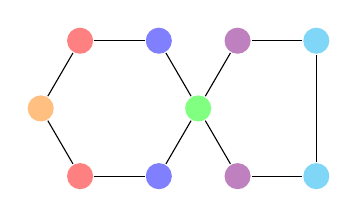
\begin{tikzpicture}
		   \begin{scope}
			   \node (0) at (1, 0)[pointgreen] {};
			   \node (1) at (0.5, 0.86)[pointblue] {};
			   \node (2) at (-0.5, 0.86)[pointred] {};
			   \node (3) at (-1, 0)[point, color=orange!50] {};
			   \node (4) at (-0.5, -0.86)[pointred] {};
			   \node (5) at (0.5, -0.86)[pointblue] {};
			   \node (6) at (1.5, -0.86)[point, color=violet!50] {};
			   \node (7) at (2.5, -0.86)[point, color=cyan!50] {};
			   \node (8) at (2.5, 0.86)[point, color=cyan!50] {};
			   \node (9) at (1.5, 0.86)[point, color=violet!50] {};
		   \end{scope}
		   \begin{scope}
			   \path [-] (0) edge (1);
			   \path [-] (1) edge (2);
			   \path [-] (2) edge (3);
			   \path [-] (3) edge (4);
			   \path [-] (4) edge (5);
			   \path [-] (5) edge (0);
			   \path [-] (0) edge (6);
			   \path [-] (6) edge (7);
			   \path [-] (7) edge (8);
			   \path [-] (8) edge (9);
			   \path [-] (9) edge (0);
		   \end{scope}
	   \end{tikzpicture}
	   \hspace{40pt}
	   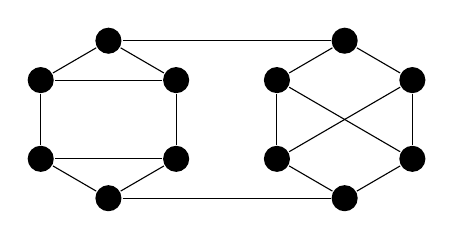
\begin{tikzpicture}
		   \begin{scope}
			   \node (0) at (0, 1)[point] {};
			   \node (1) at (0.86, 0.5)[point] {};
			   \node (2) at (0.86, -0.5)[point] {};
			   \node (3) at (0, -1)[point] {};
			   \node (4) at (-0.86, -0.5)[point] {};
			   \node (5) at (-0.86, 0.5)[point] {};
			   \node (6) at (3, 1)[point] {};
			   \node (7) at (3.86, 0.5)[point] {};
			   \node (8) at (3.86, -0.5)[point] {};
			   \node (9) at (3, -1)[point] {};
			   \node (10) at (2.14, -0.5)[point] {};
			   \node (11) at (2.14, 0.5)[point] {};
		   \end{scope}
		   \begin{scope}
			   \path [-] (0) edge (1);
			   \path [-] (1) edge (2);
			   \path [-] (2) edge (3);
			   \path [-] (3) edge (4);
			   \path [-] (4) edge (5);
			   \path [-] (5) edge (0);
			   \path [-] (6) edge (7);
			   \path [-] (7) edge (8);
			   \path [-] (8) edge (9);
			   \path [-] (9) edge (10);
			   \path [-] (10) edge (11);
			   \path [-] (11) edge (6);
			   \path [-] (0) edge (6);
			   \path [-] (3) edge (9);
			   \path [-] (1) edge (5);
			   \path [-] (2) edge (4);
			   \path [-] (7) edge (10);
			   \path [-] (8) edge (11);
		   \end{scope}
	   \end{tikzpicture}
	   \caption{Primer najgrubljeg ekvitabilnog bojenja dva grafa.}
	   \label{img:coarsesteq}
   \end{figure}

  
  Ovim smo pokazali da postoji najgrublje ekvitabilno bojenje finije od $\pi$
  određeno do na raspored ćelija. Definišimo onda funkciju $F(G, \pi, \nu)$ kao
  rezultat izvršavanja algoritma određivanja jednog takvog bojenja.

  \begin{algorithm}[H]
	  \textbf{Ulaz} Obojen graf $(G, \pi)$, čvor stabla $\nu$\\
	  \textbf{Izlaz} Najgrublje ekvitabilno bojenje finije od $\pi$
	  \caption{Profinjavanje bojenja}
	  \begin{algorithmic}[1]
		  \Procedure{Refine}{$G, \pi, \nu$}
		  \State {$\alpha \gets \emptyset$}
		  \If {$\nu = \nu' \| w$}
			\State {push($\alpha$, $\{w\}$)}
		  \Else
			\State {push($\alpha$, $C$) za sve $C \in \pi$}
		  \EndIf
		  \While{$\alpha \neq \emptyset$}
			\State {$W \gets $ pop($\alpha$)}
			\For{$C \in \pi$}
			  \State {$\pi, C_1, \dots, C_k, s \gets $ Refine\_cell($G, \pi, \pi(C), t_v = \widetilde{\psi}(G, v, W)$)}
			  \If{$C \in \alpha$}
				\State {remove($\alpha$, $C$)}
				\State {push($\alpha$, $C_i$) za sve $1 \leq i \leq k$}
			  \Else
			    \State {push($\alpha$, $C_i$) za sve $1 \leq i \leq k, i \neq s$}
			  \EndIf
			\EndFor
		  \EndWhile
		  \State \Return{$\pi$}
		  \EndProcedure
	  \end{algorithmic}
  \end{algorithm}

  Potrebno je da procedure koje modifikuju strukturu $\alpha$ budu
  implementirane na način koji garantuje invarijantnost na imenovanje čvorova.
  Ovo se jednostavno postiže bilo kojom implementacijom koja ne zavisi od
  sadržaja elemenata unutar skupa $\alpha$ poput steka ili reda, ili opštije
  implementacijom koja zavisi jedino od svojstava elemenata invarijantnih
  na imenovanje čvorova.

  \begin{theorem}
	  Neka je $\gamma$ bojenje dobijeno izvršavanjem algoritma profinjavanja
	  bojenja za ulaz $(G, \pi, \nu)$ u obojenom grafu $(G, \pi_0)$. Tada
	  $\gamma$ ispunjava uslove leme \ref{lemma:coarsesteq}.
  \end{theorem}

  \begin{proof}

	  Označimo sa $\xi$ particiju koja ispunjava uslove leme
	  \ref{lemma:coarsesteq}. Dokažimo indukcijom po $i$ da je $\xi \leq
	  \sim_{\pi_i}$ gde $\pi_i$ predstavlja bojenje $\pi$ nakon $i$ izvršenih
	  koraka spoljne petlje algoritma. Iz ovoga će slediti $\xi \leq \sim_\gamma$.

	  \begin{itemize}
		  \item[] \textbf{Baza indukcije} Po definiciji $\xi$ je $\xi \leq \sim_{\pi}$.
		  \item[] \textbf{Induktivni korak} Neka je $\xi \leq \sim_{\pi_j}$ za sve $ j \leq i$.
			  Tada je svaka ćelija $C$ svakog bojenja $\pi_j,\ j \leq i$ unija nekih
			  klasa particije $\xi$, pa to važi i za ćeliju $W$ odabranu u
			  liniji 8 algoritma.  Neka su $x$ i $y$ proizvoljni elementi iste klase
			  particije $\xi$. Tada je $\widetilde{\psi}(G, x, W) = \widetilde{\psi}(G, y, W)$, pa oni ne
			  mogu biti razdvojeni nakon izvršavanja koraka spoljne petlje.
			  Prema tome je $\xi \leq \sim_{\pi_{i+1}}$.
	  \end{itemize}

	  Neka je $C$ ćelija nekog bojenja i neka su $C_1, C_2, \dots, C_k$ ćelije
	  dobijene netrivijalnim profinjavanjem $C$ u odnosu na neku ćeliju $W$ ili
	  individualizacijom ćelije $C$. Možemo formirati šumu (skup stabala) čiji
	  su čvorovi ćelije na sledeći način:
	  \begin{enumerate}
		  \item Koren svakog stabla šume je jedna ćelija bojenja $\pi_0$ ako je
			  $\nu = ()$, odnosno $R(G, \pi_0, \nu')$ ako je $\nu = \nu' \| w$.
		  \item Deca čvora $C$ su $\{C_1, \dots, C_k\}$.
	  \end{enumerate}

	  Pokažimo da je $\gamma$ ekvitabilno. Dokaz izvodimo iz dva dela. Prvo,
	  pokažimo da važi sledeće tvrđenje. Ako je ćelija $C$ prilikom izvršavanja
	  algoritma dodata u $\alpha$ u liniji 4, 6, 13 ili 15 algoritma (u oznaci
	  $C \in \mathcal{A}$), tada se ona može predstaviti kao disjunktna unija
	  $C = W_1 \sqcup \dots \sqcup W_m$ nekih ćelija $W_1, \dots, W_m \in
	  \mathcal{W}$ gde $\mathcal{W}$ predstavlja skup svih ćelija uklonjenih iz
	  $\alpha$ linijom 8 algoritma.  Dokaz izvodimo indukcijom po strukturi
	  stabla, odozdo naviše.

	  \begin{itemize}
		  \item[] \textbf{Baza indukcije} Ukoliko je $C \in \mathcal{W}$,
			  tvrđenje važi trivijalno.
		  \item[] \textbf{Induktivni korak} Kako je po završetku izvršavanja
			  algoritma $\alpha$ prazan skup, $C$ je moralo biti uklonjeno.
			  Kako $C$ nije uklonjeno linijom 8, moralo je biti uklonjeno
			  linijom 12. U tom slučaju je $C = C_1 \sqcup \dots \sqcup C_k$ i
			  $C_1, \dots, C_k$ su dodate u $\alpha$ linijom 13. Po induktivnoj
			  hipotezi se svaki od $C_1, \dots, C_k$ može predstaviti kao
			  disjunktna unija skupova iz $\mathcal{W}$, pa to važi i za $C$.
	  \end{itemize}

	  Definišimo $\mathcal{B} = \{C \in \mathcal{P}(V) \mid \forall x, y \
	  \gamma(x) = \gamma(y) \implies \widetilde{\psi}(G, x, C) = \widetilde{\psi}(G, y, C)\}$. Jasno je da je
	  $\mathcal{W} \subseteq \mathcal{B}$. Prema prethodno pokazanom je onda i
	  $\mathcal{A} \subseteq \mathcal{B}$.  Pokažimo da za svaku ćeliju $C$ u šumi važi
	  da je $C \in \mathcal{B}$. Dokaz izvodimo indukcijom po strukturi stabla,
	  odozgo naniže.

	  \begin{itemize}
		  \item[] \textbf{Baza indukcije} Neka je $C$ koren nekog stabla šume.
			  \begin{itemize}
				  \item[1\degree] Ako je $\nu = ()$, važi $C \in \mathcal{B}$ jer je
					  dodato u $\alpha$ u liniji 6 algoritma.
				  \item[2\degree] Ako je $\nu = \nu' \| w$, bojenje $R(G,
					  \pi_0, \nu')$ je ekvitabilno, pa kako je $\gamma \leq
					  R(G, \pi_0, \nu')$, sve njegove ćelije su u $\mathcal{B}$, a
					  samim tim je i $C$.
			  \end{itemize}
		  \item[] \textbf{Induktivni korak} Neka je $C \in \mathcal{B}$ i $C = C_1 \sqcup \dots \sqcup C_k$.
			  \begin{itemize}
				  \item[1\degree] Ako je $C \in \mathcal{A}$, onda su i $C_1, \dots,
					  C_k \in \mathcal{A} \subseteq \mathcal{B}$.
				  \item[2\degree] Ako je $C \not \in \mathcal{A}$, onda su $C_1,
					  \dots, C_{s-1}, C_{s+1}, \dots, C_k \in \mathcal{A} \subseteq
					  \mathcal{B}$. Tada je $\widetilde{\psi}(G, x, C_s) = \widetilde{\psi}(G, x, C) -
					  \sum_{1 \leq i \leq k, i \neq s} \widetilde{\psi}(G, x, C_i)$, pa je
					  i $C_s \in \mathcal{B}$.
			  \end{itemize}
	  \end{itemize}

	  Kako su sve ćelije šume u $\mathcal{B}$, to su i sve ćelije bojenja $\gamma$,
	  pa je $\gamma$ ekvitabilno.
  \end{proof}

  \begin{theorem}
	  Neka je $\nu$ list stabla $\mathcal{T}(G, \pi)$. Tada je postupak
	  određivanja $R(G, \pi, [\nu]_i)$ za sve $0 \leq i \leq |\nu|$ ukupne
	  vremenske složenosti $O(n^2 \log n)$, pri čemu je $n$ broj čvorova grafa.
  \end{theorem}

  \begin{proof}
	  Pretpostavimo da su operacije \texttt{push}, \texttt{pop} i
	  \texttt{remove} složenosti $O(1)$. Za fiksno $W$ i $C$ broj koraka jedne
	  iteracije unutrašnje petlje je $|C||W| + |C| \log |C| + k \leq |C||W| +
	  |C| (1 + \log |C|)$ za određivanje vrednosti $t_v$ za svaki čvor ćelije
	  $C$, izvršavanje profinjavanja ćelije $C$ i dodavanje svih potrebnih
	  $C_i$ u $\alpha$. Dakle, za fiksno $W$ je broj koraka unutrašnje petlje
	  manji ili jednak $\sum_{C \in \pi}(|C||W| + |C| (1 + \log |C|)) \leq
	  \sum_{C \in \pi}(|C||W| + |C| (1 + \log n)) = n|W| + n(1 + \log n)$.
	  Odatle je broj koraka za određivanje $R(G, \pi, [\nu]_i)$ najviše
	  $\sum_{W \in \mathcal{W}_i} (n|W| + n(1 + \log n)) = n \sum_{W \in
	  \mathcal{W}_i} |W| + |\mathcal{W}_i| n (1 + \log n)$ gde je
	  $\mathcal{W}_i$ skup svih ćelija na osnovu kojih je vršeno profinjavanje
	  prilikom određivanja $R(G, \pi, [\nu]_i)$, odnosno svih ćelija $W$ iz
	  linije 8 algoritma. Ukupna složenost svih profinjavanja je onda
	  $\sum_{i=1}^{|\nu|}(n \sum_{W \in \mathcal{W}_i} |W| + |\mathcal{W}_i| n
	  (1 + \log n)) = O(n \sum_{W \in \mathcal{W}} |W| + |\mathcal{W}| n \log
	  n)$ pri čemu je $\mathcal{W} = \bigcup_{i = 1}^{|\nu|}\mathcal{W}_i$.

	  Neka je $C$ ćelija nekog bojenja i neka su $C_1, C_2, \dots, C_k$ ćelije
	  dobijene netrivijalnim profinjavanjem $C$ u odnosu na neku ćeliju $W$ ili
	  individualizacijom ćelije $C$. Možemo formirati šumu (skup stabala) čiji
	  su čvorovi ćelije na sledeći način:
	  \begin{enumerate}
		  \item Koren svakog stabla šume je jedna ćelija bojenja $R(G, \pi, ())$.
		  \item Deca čvora $C$ su $\{C_1, \dots, C_k\}$.
	  \end{enumerate}

	  Kako su ćelije u listovima šume sve različite jednočlane ćelije (jer je
	  bojenje $R(G, \pi, \nu)$ diskretno), ima ih tačno $n$. Kako svaka ćelija
	  šume ima bar dva deteta, broj ćelija u šumi je manji od $2n$, a pošto ona
	  mora sadržati i sve ćelije iz $\mathcal{W}$, to je $|\mathcal{W}| < 2n$.

	  Neka je $v$ čvor grafa. Posmatrajmo niz ćelija $\{v\} = C_m \subseteq
	  C_{m-1} \subseteq \dots \subseteq C_1$ koje čine put od lista $\{v\}$ do
	  korena odgovarajućeg stabla. Neka je ćelija $C_i$ jedna od ćelija dodatih
	  u $\alpha$ u liniji 4, 6, ili 15 algoritma. Tada je $|C_i| \leq
	  \frac{|C_{i-1}|}{2}$ ako je $i > 1$, odnosno nakon individualizacije ili
	  profinjavanja. Označimo broj ovakvih ćelija sa $k_v$. Očigledno je $k_v
	  \leq 1 + \log_2 |C_1| \leq 1 + \log_2 n$.

	  Primetimo da su u svakom koraku algoritma ćelije koje se nalaze u
	  $\alpha$ međusobno disjunktne. Odavde sledi da se istovremeno u $\alpha$
	  ne mogu naći dve različite ćelije $C_i$ i $C_j$. Primetimo, takođe, da
	  jedino linije 4, 6, 8 i 15 algoritma mogu da promene tačnost rečenice
	  $\exists i \ C_i \in \alpha$ (12 i 13 ne mogu ukoliko se posmatraju
	  zajedno). Kako je na početku i na kraju izvršavanja algoritma $\alpha =
	  \emptyset$, mora važiti da je broj $k_v$ dodavanja ćelija $C_i$ u $\alpha$
	  jednak broju uklanjanja ćelija $C_i$ iz $\alpha$, odnosno broju onih ćelija za
	  koje važi $C_i \in \mathcal{W}$.

	  Konačno,
	  \begin{align*}
		  \sum_{W \in \mathcal{W}} |W| &= \sum_{W \in \mathcal{W}} \sum_{v \in W} 1\\
		  &= \sum_{W \in \mathcal{W}} \sum_{v \in V} \chi_W(v)\\
		  &= \sum_{v \in V} \sum_{W \in \mathcal{W}} \chi_W(v) \\
		  &= \sum_{v \in V} k_v\\
		  &\leq \sum_{v \in V} (1 + \log_2 n)\\
		  &= n (1 + \log_2 n)
	  \end{align}
	  gde je $\chi_W : V \to \{0, 1\}$ karakteristična funkcija skupa $W$.
  \end{proof}

   \begin{figure}[htp]
	   \centering
	   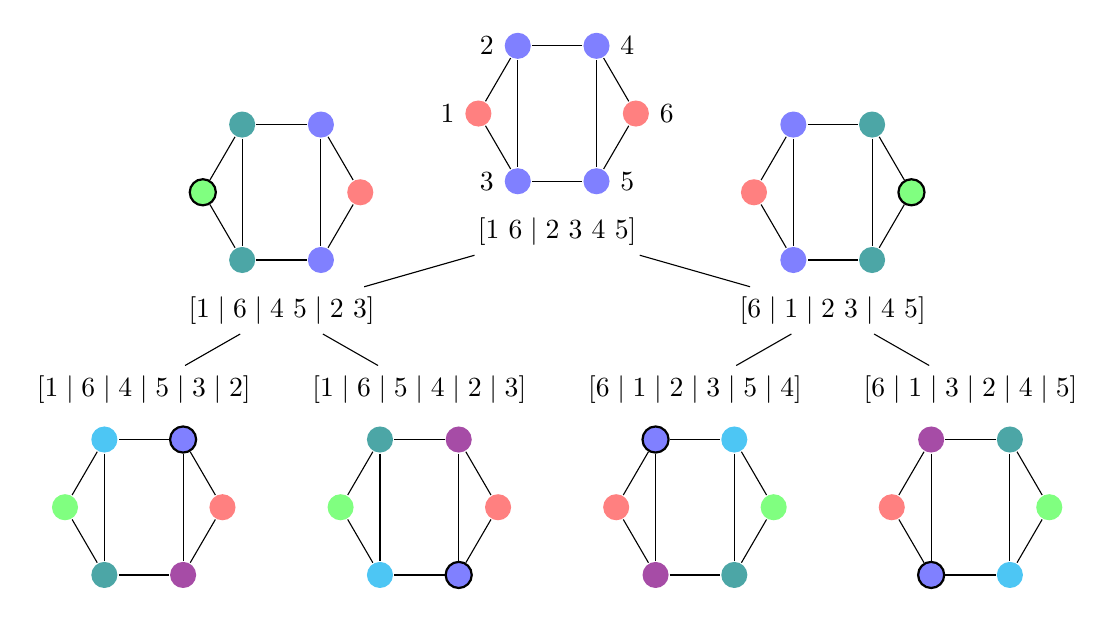
\begin{tikzpicture}
		   \begin{scope}
			   \node (0) at (0, 0) {$[1\ 6 \mid 2\ 3\ 4\ 5]$};
			   \node (1) at (-3.5, -1) {$[1 \mid 6 \mid 4\ 5 \mid 2\ 3]$};
			   \node (6) at (3.5, -1) {$[6 \mid 1 \mid 2\ 3 \mid 4\ 5]$};
			   \node (14) at (-5.25, -2) {$[1 \mid 6 \mid 4 \mid 5 \mid 3 \mid 2]$};
			   \node (15) at (-1.75, -2) {$[1 \mid 6 \mid 5 \mid 4 \mid 2 \mid 3]$};
			   \node (62) at (1.75, -2) {$[6 \mid 1 \mid 2 \mid 3 \mid 5 \mid 4]$};
			   \node (63) at (5.25, -2) {$[6 \mid 1 \mid 3 \mid 2 \mid 4 \mid 5]$};

			   \node (a1) at (1, 1.5)[pointred, label=0:6] {};
			   \node (a2) at (0.5, 2.36)[pointblue, label=0:4] {};
			   \node (a3) at (-0.5, 2.36)[pointblue, label=180:2] {};
			   \node (a4) at (-1, 1.5)[pointred, label=180:1] {};
			   \node (a5) at (-0.5, 0.64)[pointblue, label=180:3] {};
			   \node (a6) at (0.5, 0.64)[pointblue, label=0:5] {};

			   \node (b1) at (-2.5, 0.5)[pointred] {};
			   \node (b2) at (-3, 1.36)[pointblue] {};
			   \node (b3) at (-4, 1.36)[point, color=teal!70] {};
			   \node (b4) at (-4.5, 0.5)[pointgreen, draw] {};
			   \node (b5) at (-4, -0.36)[point, color=teal!70] {};
			   \node (b6) at (-3, -0.36)[pointblue] {};

			   \node (c1) at (2.5, 0.5)[pointred] {};
			   \node (c2) at (3, 1.36)[pointblue] {};
			   \node (c3) at (4, 1.36)[point, color=teal!70] {};
			   \node (c4) at (4.5, 0.5)[pointgreen, draw] {};
			   \node (c5) at (4, -0.36)[point, color=teal!70] {};
			   \node (c6) at (3, -0.36)[pointblue] {};

			   \node (d1) at (-4.25, -3.5)[pointred] {};
			   \node (d2) at (-4.75, -2.64)[pointblue, draw] {};
			   \node (d3) at (-5.75, -2.64)[point, color=cyan!70] {};
			   \node (d4) at (-6.25, -3.5)[pointgreen] {};
			   \node (d5) at (-5.75, -4.36)[point, color=teal!70] {};
			   \node (d6) at (-4.75, -4.36)[point, color=violet!70] {};

			   \node (e1) at (-0.75, -3.5)[pointred] {};
			   \node (e2) at (-1.25, -2.64)[point, color=violet!70] {};
			   \node (e3) at (-2.25, -2.64)[point, color=teal!70] {};
			   \node (e4) at (-2.75, -3.5)[pointgreen] {};
			   \node (e5) at (-2.25, -4.36)[point, color=cyan!70] {};
			   \node (e6) at (-1.25, -4.36)[pointblue, draw] {};

			   \node (f1) at (2.75, -3.5)[pointgreen] {};
			   \node (f2) at (2.25, -2.64)[point, color=cyan!70] {};
			   \node (f3) at (1.25, -2.64)[pointblue, draw] {};
			   \node (f4) at (0.75, -3.5)[pointred] {};
			   \node (f5) at (1.25, -4.36)[point, color=violet!70] {};
			   \node (f6) at (2.25, -4.36)[point, color=teal!70] {};

			   \node (g1) at (6.25, -3.5)[pointgreen] {};
			   \node (g2) at (5.75, -2.64)[point, color=teal!70] {};
			   \node (g3) at (4.75, -2.64)[point, color=violet!70] {};
			   \node (g4) at (4.25, -3.5)[pointred] {};
			   \node (g5) at (4.75, -4.36)[pointblue, draw] {};
			   \node (g6) at (5.75, -4.36)[point, color=cyan!70] {};

		   \end{scope}
		   \begin{scope}
			   \path [-] (0) edge (1);
			   \path [-] (0) edge (6);
			   \path [-] (1) edge (14);
			   \path [-] (1) edge (15);
			   \path [-] (6) edge (62);
			   \path [-] (6) edge (63);

			   \path [-] (a1) edge (a2);
			   \path [-] (a2) edge (a3);
			   \path [-] (a3) edge (a4);
			   \path [-] (a4) edge (a5);
			   \path [-] (a5) edge (a6);
			   \path [-] (a6) edge (a1);
			   \path [-] (a2) edge (a6);
			   \path [-] (a3) edge (a5);

			   \path [-] (b1) edge (b2);
			   \path [-] (b2) edge (b3);
			   \path [-] (b3) edge (b4);
			   \path [-] (b4) edge (b5);
			   \path [-] (b5) edge (b6);
			   \path [-] (b6) edge (b1);
			   \path [-] (b2) edge (b6);
			   \path [-] (b3) edge (b5);

			   \path [-] (c1) edge (c2);
			   \path [-] (c2) edge (c3);
			   \path [-] (c3) edge (c4);
			   \path [-] (c4) edge (c5);
			   \path [-] (c5) edge (c6);
			   \path [-] (c6) edge (c1);
			   \path [-] (c2) edge (c6);
			   \path [-] (c3) edge (c5);

			   \path [-] (d1) edge (d2);
			   \path [-] (d2) edge (d3);
			   \path [-] (d3) edge (d4);
			   \path [-] (d4) edge (d5);
			   \path [-] (d5) edge (d6);
			   \path [-] (d6) edge (d1);
			   \path [-] (d2) edge (d6);
			   \path [-] (d3) edge (d5);

			   \path [-] (e1) edge (e2);
			   \path [-] (e2) edge (e3);
			   \path [-] (e3) edge (e4);
			   \path [-] (e4) edge (e5);
			   \path [-] (e5) edge (e6);
			   \path [-] (e6) edge (e1);
			   \path [-] (e2) edge (e6);
			   \path [-] (e3) edge (e5);

			   \path [-] (f1) edge (f2);
			   \path [-] (f2) edge (f3);
			   \path [-] (f3) edge (f4);
			   \path [-] (f4) edge (f5);
			   \path [-] (f5) edge (f6);
			   \path [-] (f6) edge (f1);
			   \path [-] (f2) edge (f6);
			   \path [-] (f3) edge (f5);

			   \path [-] (g1) edge (g2);
			   \path [-] (g2) edge (g3);
			   \path [-] (g3) edge (g4);
			   \path [-] (g4) edge (g5);
			   \path [-] (g5) edge (g6);
			   \path [-] (g6) edge (g1);
			   \path [-] (g2) edge (g6);
			   \path [-] (g3) edge (g5);

		   \end{scope}
	   \end{tikzpicture}
	   \caption{Stablo pretrage generisano definisanom funkcijom profinjavanja.}
	   \label{img:refinedtree}
   \end{figure}

  \begin{example}
	  Na slici \ref{img:refinedtree} prikazano je stablo pretrage jednobojnog
	  grafa koje koristi definisanu funkciju profinjavanja. Prikazan je obojen
	  graf nakon svakog profinjavanja i zaokruženi su čvorovi korišćeni
	  prilikom individualizacije. U korenu stabla se profinjavanjem dobija
	  ekvitabilno bojenje sa dve boje, razdvajanjem čvorova stepena dva i tri.
	  U narednom nivou stabla se vrši individualizacija jednog od čvorova
	  stepena dva pri čemu se profinjavanjem čvorovi stepena tri dele u dve
	  ćelije po tome da li su povezani sa individualizovanim čvorom ili ne. U
	  poslednjem nivou se vrši individualizacija jednog od čvorova stepena tri
	  koji nije sused prethodno individualizovanom čvoru i profinjavanjem se
	  dolazi do diskretnog bojenja.
  \end{example}


 \section{Invarijanta stabla}

  \begin{lemma}
	  Neka je $f : \mathcal{G} \times \Pi \times V^* \to F$ funkcija
	  invarijantna na imenovanje čvorova, pri čemu je $F$ neki potpuno uređen
	  skup i neka je $bin(G)$ binarna reprezentacija gornjeg trougla matrice
	  povezanosti grafa $G$. Tada je funkcija definisana sa
	  $$ \phi(G, \pi, \nu) =
	  \begin{cases}
		  (f(G, \pi, [\nu]_0), \dots, f(G, \pi, [\nu]_{|\nu|})), & \ \text{ako } \pi_\nu \text{ nije diskretno} \\
		  (f(G, \pi, [\nu]_0), \dots, f(G, \pi, [\nu]_{|\nu|}), bin(G^{\pi_\nu})), & \ \text{inače}
	  \end{cases}
	  $$ invarijanta stabla pri leksikografskom poretku.
  \end{lemma}

  \begin{proof}
	  Dokažimo da tako definisana funkcija $\phi$ ispunjava uslove invarijante stabla.
	  \begin{itemize}
		  \item[(\phi1)] Za svaki čvor $\omega$ podstabla $\mathcal{T}(G, \pi,
			  \nu)$ važi da je $\phi(G, \pi, \nu) = [\phi(G, \pi,
			  \omega)]_{|\nu|}$. Neka su $\nu_1$ i $\nu_2$ čvorovi stabla takvi
			  da je $|\nu_1|=|\nu_2|$ i $\phi(G, \pi, \nu_1) < \phi(G, \pi,
			  \nu_2)$. Tada za čvorove $\omega_1 \in \mathcal{T}(G, \pi,
			  \nu_1)$ i $\omega_2 \in \mathcal{T}(G, \pi, \nu_2)$ važi
			  $[\phi(G, \pi, \omega_1)]_{|\nu_1|} < [\phi(G, \pi,
			  \omega_2)]_{|\nu_2|}$ pa je po leksikografskom poretku i $\phi(G,
			  \pi, \omega_1) < \phi(G, \pi, \omega_2)$.
		  \item[(\phi2)] Ako za listove $\nu_1$ i $\nu_2$ važi $\phi(G, \pi,
			  \nu_1) = \phi(G, \pi, \nu_2)$, onda je $bin(G^{\pi_1}) =
			  bin(G^{\pi_2})$, pa je $G^{\pi_1} = G^{\pi_2}$.
		  \item[(\phi3)] Neka je $g \in Aut(G, \pi)$ i $\nu$ čvor stabla. Tada
			  je $f(G^g, \pi^g, [\nu^g]_i) = f(G^g, \pi^g, [\nu]_i^g) = f(G,
			  \pi, [\nu]_i)$, kao i $bin((G^g)^{R(G^g, \pi^g, \nu^g)}) =
			  bin((G^g)^{\pi_\nu^g}) = bin(G^{\pi_\nu})$, pa su nizovi
			  $\phi(G^g, \pi^g, \nu^g)$ i $\phi(G, \pi, \nu)$ jednaki.
	  \end{itemize}
  \end{proof}

  Još je potrebno odabrati konkretnu funkciju $f$. Uvedimo za početak pojam
  \emph{količničkog grafa}.

  \begin{definition}
	  Neka je $(G, \pi)$ obojen graf i $\pi$ ekvitabilno. \emph{Količnički
	  graf} $Q(G, \pi) = (V_Q, d_Q, \psi_Q)$ je struktura takva da je $V_Q$
	  skup od $|\pi|$ čvorova, $d_Q : V_Q \to \mathbb{N}$ preslikavanje takvo
	  da je $d_Q(c) = |\pi^{-1}(c)|$ i $\psi_Q : V_Q^2 \to \mathbb{N}$
	  preslikavanje takvo da važi $\psi_Q(c_1, c_2) = \widetilde{\psi}(G, v,
	  \pi^{-1}(c_2))$ za bilo koje $v \in \pi^{-1}(c_1)$.
  \end{definition}

  \begin{example}
	  Na slici \ref{img:quotient} prikazan je graf sa ekvitabilnim bojenjem i
	  odgovarajući količnički graf. Vrednosti $d_Q(c)$ odgovaraju broju čvorova
	  grafa boje $c$ i upisane su u čvorove količničkog grafa.  Vrednosti
	  $\psi_Q(c_1, c_2)$ odgovaraju broju čvorova boje $c_2$ grafa sa kojim je
	  povezan svaki čvor boje $c_1$ i napisane su pored odgovarajućih usmerenih
	  grana, dok grane kojima je ta vrednost nula nisu prikazane.
  \end{example}

   \begin{figure}[htp]
	   \centering
	   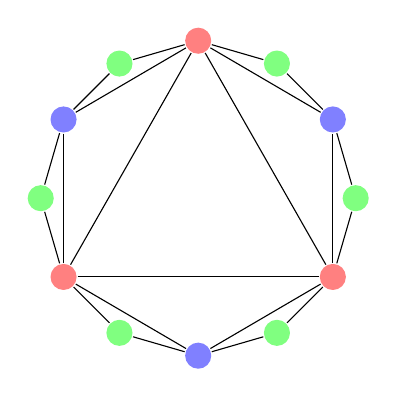
\begin{tikzpicture}
		   \begin{scope}
			   \node (0) at (2, 0)[pointgreen] {};
			   \node (1) at (1.71, 1)[pointblue] {};
			   \node (2) at (1, 1.71)[pointgreen] {};
			   \node (3) at (0,2)[pointred] {};
			   \node (4) at (-1, 1.71)[pointgreen] {};
			   \node (5) at (-1.71, 1)[pointblue] {};
			   \node (6) at (-2, 0)[pointgreen] {};
			   \node (7) at (-1.71, -1)[pointred] {};
			   \node (8) at (-1, -1.71)[pointgreen] {};
			   \node (9) at (0, -2)[pointblue] {};
			   \node (10) at (1, -1.71)[pointgreen] {};
			   \node (11) at (1.71, -1)[pointred] {};
		   \end{scope}
		   \begin{scope}
			   \path [-] (0) edge (1);
			   \path [-] (1) edge (2);
			   \path [-] (2) edge (3);
			   \path [-] (3) edge (4);
			   \path [-] (4) edge (5);
			   \path [-] (5) edge (6);
			   \path [-] (6) edge (7);
			   \path [-] (7) edge (8);
			   \path [-] (8) edge (9);
			   \path [-] (9) edge (10);
			   \path [-] (10) edge (11);
			   \path [-] (11) edge (0);
			   \path [-] (1) edge (3);
			   \path [-] (3) edge (5);
			   \path [-] (5) edge (7);
			   \path [-] (7) edge (9);
			   \path [-] (9) edge (11);
			   \path [-] (11) edge (1);
			   \path [-] (3) edge (7);
			   \path [-] (7) edge (11);
			   \path [-] (11) edge (3);
		   \end{scope}
	   \end{tikzpicture}
	   \hspace{40pt}
	   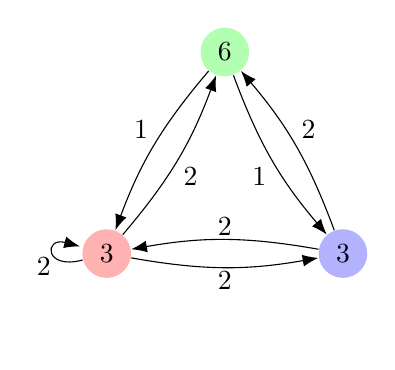
\begin{tikzpicture}
		   \begin{scope}
			   \node (0) at (0, 0)[circle, fill=red!30] {3};
			   \node (1) at (3, 0)[circle, fill=blue!30] {3};
			   \node (2) at (1.5, 2.56)[circle, fill=green!30] {6};
			   \node (3) at (0, -1) {};
		   \end{scope}
		   \begin{scope}[label distance=-2mm]
			   \path [->] (0) edge[arrow, loop left] node[label=below:2]{} (0);

			   \path [->] (0) edge[arrow, bend right = 10] node[label=below:2]{} (1);
			   \path [->] (1) edge[arrow, bend right = 10] node[label=above:2]{} (0);

			   \path [->] (1) edge[arrow, bend right = 10] node[label=30:2]{} (2);
			   \path [->] (2) edge[arrow, bend right = 10] node[label=210:1]{} (1);

			   \path [->] (0) edge[arrow, bend right = 10] node[label=-30:2]{} (2);
			   \path [->] (2) edge[arrow, bend right = 10] node[label=150:1]{} (0);
		   \end{scope}
	   \end{tikzpicture}
	   \caption{Ekvitabilno bojenje (levo) i količnički graf (desno).}
	   \label{img:quotient}
   \end{figure}


  Primetimo da je definicija dobra zbog ekvitabilnosti bojenja $\pi$. Sledeća
  lema pokazuje značaj uvedenog pojma.

  \begin{lemma}
	  Neka je $Q : \mathcal{G}_{eq} \to \mathcal{Q}$ prethodno definisano
	  preslikavanje iz skupa obojenih grafova sa ekvitabilnim bojenjem u skup
	  količničkih grafova. $Q$ je funkcija invarijantna na imenovanje čvorova.
  \end{lemma}

  \begin{proof}
	  Neka je $g \in S_n$ proizvoljno. Pokažimo da je $Q(G^g, \pi^g) = Q(G,
	  \pi)$. Kako je $|\pi^g| = |\pi|$ to su skupovi čvorova količničkih
	  grafova jednaki. Dalje, važi $d_{Q(G^g, \pi^g)}(c) = |(\pi^g)^{-1}(c)| =
	  |\pi^{-1}(c)| = d_{Q(G, \pi)}(c)$. Konačno, neka je $u' \in
	  (\pi^g)^{-1}(c_1)$. Tada važi 
	  \begin{align*}
		  \psi_{Q(G^g, \pi^g)}(c_1, c_2) &= \widetilde{\psi}(G^g, u', (\pi^g)^{-1}(c_2)) \\
		  &= \sum_{v' \in (\pi^g)^{-1}(c_2)} \psi(G^g, u', v') \\
		  &= \sum_{v^g \in (\pi^g)^{-1}(c_2)} \psi(G^g, u^g, v^g) &\text{smena }u'=u^g, v'=v^g\\
		  &= \sum_{v \in \pi^{-1}(c_2)} \psi(G^g, u^g, v^g) &(\pi^g)^{-1}(c_2) = \pi^{-1}(c_2)^g\\
		  &= \sum_{v \in \pi^{-1}(c_2)} \psi(G, u, v) &(\psi2)\\
		  &= \widetilde{\psi}(G, u, \pi^{-1}(c_2)) \\
		  &= \psi_{Q(G, \pi)}(c_1, c_2) &(\pi^g)^{-1}(c_1) = \pi^{-1}(c_1)^g
	  \end{align}
  \end{proof}

  \begin{corrolary}
	  Preslikavanje $f_Q : \mathcal{G} \times \Pi \times V^* \to \mathcal{Q}$
	  definisano sa $f_Q(G, \pi, \nu) = Q(G, R(G, \pi, \nu))$ je funkcija
	  invarijantna na imenovanje čvorova.
  \end{corrolary}

  Jasno je da za preslikavanje $f$ možemo uzeti upravo ceo količnički graf, pri
  čemu je uređenje količničkih grafova moguće realizovati uređivanjem njihovih
  binarnih reprezentacija. Ovakva definicija preslikavanja $f$ u praksi nije
  korisna zbog velike složenosti neophodne za njeno izračunavanje - potrebno je
  realizovati ceo količnički graf. Ovo je moguće rešiti posmatranjem manjeg
  dela količničkog grafa i to bez gubitka korisnih informacija.

  \begin{definition}
	  Neka je $(G, \pi)$ obojen graf i $\nu = \nu' \| w$ čvor stabla različit
	  od korena. Uvedimo oznake $\pi_1 = R(G, \pi, \nu')$ i $\pi_2 = R(G, \pi,
	  \nu)$.  Neka su $c_1, \dots, c_k$ boje takve da za sve $1 \leq i \leq k$
	  važi da $\pi_2^{-1}(c_i)$ nije ćelija bojenja $\pi_1$. Označimo sa $f_i$
	  niz vrednosti $(c_i, d_{Q(G, \pi_2)}(c_i), \psi_{Q(G, \pi_2)}(c_i, c_1),
	  \dots, \psi_{Q(G, \pi_2)}(c_i, c_k))$. Preslikavanje $f(G, \pi, \nu)$
	  čija je vrednost prazan niz $()$ u slučaju korena $\nu$, odnosno dobijena
	  nadovezivanjem nizova $f_1, \dots, f_k$ u suprotnom, zovemo
	  \emph{razlikom količničkih grafova}.
  \end{definition}

  \begin{example}
	  Posmatrajmo najlevlji list i njegovog roditelja u stablu pretrage
	  prikazanom na slici \ref{img:refinedtree}. Bojenje $[1 \mid 6 \mid 4 \mid
	  5 \mid 3 \mid 2]$ ima četiri ćelije koje nisu u bojenju $[1 \mid 6 \mid
	  4\ 5 \mid 2\ 3]$. To su $\{4\}, \{5\}, \{3\}, \{2\}$, redom za boje $c_1
	  = 3, c_2 = 4, c_3 = 5, c_4 = 6$. Tada je $f_1 = (c_1, d_{Q}(c_1),
	  \psi_Q(c_1, c_1), \psi_Q(c_1, c_2), \psi_Q(c_1, c_3), \psi_Q(c_1, c_4)) =
	  (3, 1, 0, 1, 0, 1)$. Dalje, $f_2 = (4, 1, 1, 0, 1, 0), f_3 = (5, 1, 0, 1,
	  0, 1), f_4 = (6, 1, 1, 0, 1, 0)$, pa je $f(G, \pi, \nu) = (3, 1, 0, 1, 0,
	  1, 4, 1, 1, 0, 1, 0, 5, 1, 0, 1, 0, 1, 6, 1, 1, 0, 1, 0)$.
  \end{exampel}

  \begin{lemma}
	  Razlika količničkih grafova $f$ je funkcija invarijantna na imenovanje
	  čvorova.
  \end{lemma}

  \begin{proof}
	  Pretpostavimo da za neko $g \in S_n$ i neke boje $c$ i $d$ važi
	  $\pi_2^{-1}(c) = \pi_1^{-1}(d)$, odnosno da je $\pi_2^{-1}(c)$ ćelija
	  bojenja $\pi_1$.  Tada je $R(G^g, \pi^g, \nu^g)^{-1}(c) =
	  (\pi_2^g)^{-1}(c) = \pi_2^{-1}(c)^g = \pi_1^{-1}(d)^g = (\pi_1^g)^{-1}(d)
	  = R(G^g, \pi^g, \nu'^g)^{-1}(d)$. Analogno se pokazuje i obrnuta
	  implikacija.  Ovim smo pokazali da je niz boja $c_1, \dots, c_k$ jednak
	  za $f(G^g, \pi^g, \nu^g)$ i $f(G, \pi, \nu)$. Tvrđenje onda jednostavno
	  važi pošto je količnički graf funkcija invarijantna na imenovanje
	  čvorova.
  \end{proof}

  Naredna teorema opravdava upotrebu invarijante stabla koja se ne oslanja na
  ceo količnički graf i pokazuje da ne postoji gubitak informacije prilikom
  njenog izračunavanja.

  \begin{theorem}
	  Neka je $(G, \pi)$ obojen graf i $\nu \| w_1$ i $\nu \| w_2$ različiti
	  čvorovi stabla. Tada je $f(G, \pi, \nu \| w_1) = f(G, \pi, \nu \| w_2)$
	  ako i samo ako $f_Q(G, \pi, \nu \| w_1) = f_Q(G, \pi, \nu \| w_2)$.
  \end{theorem}
  
  \begin{proof}
	  Dokaz implikacije ulevo je trivijalan. Za smer udesno dokazaćemo
	  kontrapoziciju tvrđenja.

	  Uvedimo oznake $\pi_1 = R(G, \pi, \nu \| w_1)$ i $\pi_2 = R(G, \pi, \nu \|
	  w_2)$. Pretpostavimo da je $Q(G, \pi_1) \neq Q(G, \pi_2)$. Ako je
	  $V_{Q(G, \pi_1)} \neq V_{Q(G, \pi_2)}$ ili $d_{Q(G, \pi_1)} \neq d_{Q(G,
	  \pi_2)}$ onda je skup ćelija bojenja $\pi_1$ i $\pi_2$ koje nisu ćelije u
	  $\pi_\nu$ različit, pa je $f(G, \pi, \nu \| w_1) \neq f(G, \pi, \nu \|
	  w_2)$. Ako je $\psi_{Q(G, \pi_1)}(c_1, c_2) \neq \psi_{Q(G, \pi_2)}(c_1,
	  c_2)$ za neke $c_1$ i $c_2$ čije odgovarajuće ćelije iz $\pi_1$ i $\pi_2$
	  nisu ćelije bojenja $\pi_\nu$, očigledno je $f(G, \pi, \nu \| w_1) \neq
	  f(G, \pi, \nu \| w_2)$.

	  Pretpostavimo da je $\pi_1^{-1}(c_2)$ ćelija bojenja $\pi_\nu$. Tada zbog
	  ekvitabilnosti bojenja $\pi_\nu$ za proizvoljno $c_1$ važi $\psi_{Q(G,
	  \pi_1)}(c_1, c_2) = \psi_{Q(G, \pi_\nu)}(d_1, d_2)$ gde je $d_1$ takvo da
	  je $\pi_1^{-1}(c_1) \subseteq \pi_\nu^{-1}(d_1)$, a $d_2$ takvo da je
	  $\pi_1^{-1}(c_2) = \pi_\nu^{-1}(d_2)$. Odatle sledi da ne važi
	  $\psi_{Q(G, \pi_1)}(c_1, c_2) \neq \psi_{Q(G, \pi_2)}(c_1, c_2)$ jer je
	  $\psi_{Q(G, \pi_1)}(c_1, c_2) = \psi_{Q(G, \pi_\nu)}(d_1, d_2) =
	  \psi_{Q(G, \pi_2)}(c_1, c_2)$, a znamo da su u obe jednakosti isti $d_1$
	  i $d_2$ u pitanju jer su $\pi_1, \pi_2 \leq \pi_\nu$.

	  Pretpostavimo da je $\pi_1^{-1}(c_1)$ ćelija bojenja $\pi_\nu$. Tada ne važi
	  $\psi_{Q(G, \pi_1)}(c_1, c_2) \neq \psi_{Q(G, \pi_2)}(c_1, c_2)$ zato što
	  po prethodno pokazanom važi $|\pi_1^{-1}(c_1)|\psi_{Q(G, \pi_1)}(c_1,
	  c_2) = |\pi_1^{-1}(c_2)|\psi_{Q(G, \pi_1)}(c_2, c_1) =
	  |\pi_2^{-1}(c_2)|\psi_{Q(G, \pi_2)}(c_2, c_1) =
	  |\pi_2^{-1}(c_1)|\psi_{Q(G, \pi_2)}(c_1, c_2)$.

	  Dokažimo još korišćeno svojstvo $|C_1|\psi_{Q(G, \pi)}(c_1, c_2) =
	  |C_2|\psi_{Q(G, \pi)}(c_2, c_1)$ za $C_1 = \pi^{-1}(c_1)$ i $C_2 =
	  \pi^{-1}(c_2)$. Ono važi zato što za svako $u \in C_1$ važi
	  $|C_1|\psi_{Q(G, \pi)}(c_1, c_2) = |C_1|\widetilde{\psi}(G, u, C_2) =
	  \sum_{u \in C_1} \widetilde{\psi}(G, u, C_2) = \sum_{u \in C_1} \sum_{v
	  \in C_2} \psi(G, u, v)$. Iz simetričnosti $(\psi1)$ i mogućnosti zamene
	  mesta suma sledi tražena jednakost.
  \end{proof}

  Primetimo da je vremenska složenost određivanja invarijante u čvoru $\nu \|
  w$ u klasi $O((|\pi_2| - |\pi_1|)n)$ gde je $\pi_2 = R(G, \pi, \nu \| w)$,
  $\pi_1 = R(G, \pi, \nu)$ i $n$ broj čvorova grafa. Ovo se jednostavno vidi iz
  toga što je broj ćelija $\pi_2$ koje nisu ćelije $\pi_1$ upravo $|\pi_2| -
  |\pi_1|$ i iz toga što je za određivanje svakog niza $f_i$ dovoljno $O(n)$
  koraka. To znači da ukupna složenost određivanja svih invarijanti od korena
  do jednog od listova stabla pripada klasi $O(n^2)$.

 \section{Automorfizmi}

  Prilikom pretrage otkrivaju se automorfizmi koji se dalje koriste za
  odsecanje. Ako je poznat skup automorfizama $\{g_1, \dots, g_n\}$, u
  operaciji odsecanja $P_C$ moguće je primeniti ne samo neki od tih
  automorfizama, već i proizvoljan automorfizam iz grupe generisane tim skupom.
  
  Operacija odsecanja $P_C$ se primenjuje što je ranije u stablu moguće.
  Konkretno, neka je $\nu = (v_1, \dots, v_{|\nu|})$ i neka je $k$ dužina
  najdužeg zajedničkog prefiksa nizova $\nu$ i $\nu^g$ za neki automorfizam
  $g$. Tada je moguće primeniti operaciju odsecanja $P_C([\nu]_{k+1}, g)$.
  Primetimo da $g$ stabilizuje niz $[\nu]_k$, odnosno $g \in \Sigma_{[\nu]_k}$
  i da stoga $v_{k+1}$ i $v_{k+1}^g$ pripadaju istoj orbiti tog stabilizatora.

  Zbog ovoga je korisno na efikasan način realizovati određivanje stabilizatora
  (ili nekog njegovog podskupa) i određivanje orbita nekog skupa automorfizama.
  Pored samog skupa automorfizama čuvaju se podaci koji ovo i omogućavaju.

  Neka je $S = \{g_1, \dots, g_n\}$ skup automorfizama. Definišimo $stab_S(v) =
  \{g \in S \mid v^{g} = v\}$. Grupa automorfizama generisana skupom $S_\nu =
  \bigcap_{1 \leq j \leq k} stab_S(v_j)$ je podgrupa stabilizatora niza $\nu =
  (v_1, \dots, v_k)$, odnosno $\langle S_\nu \rangle \leq \Sigma^{Aut(G,
  \pi)}_\nu = Aut(G, \pi_\nu)$.

  Definišimo $mcr_S(v) = \min \Omega_v^{\langle S \rangle}$. Neka je $\nu$ čvor stabla.
  Kako je prema prethodno pokazanom $P_C$ moguće primenjivati za bilo koja dva
  čvora iz iste orbite stabilizatora, možemo odseći pretragu u bilo kom čvoru
  $\nu \| v$ za koji važi $v \neq mcr_{S_\nu}(v)$.

  Prilikom dodavanja novog automorfizma $g$ u skup potrebno je ažurirati ove
  podatke. Skupovi $stab_S(v)$ se jednostavno ažuriraju dodavanjem $g$ tamo gde
  je potrebno. Kako bi se ažuriranje predstavnika orbita moglo efikasno
  izvršiti, pamti se pomoćna particija $\Omega$ čvorova po orbitama. Prilikom
  dodavanja se nova particija određuje kao supremum particije $\Omega$ i
  particije ciklusa (orbita) automorfizma $g$.  Proizvoljnu particiju moguće je
  preslikati u odgovarajući graf formiranjem prostog ciklusa nad elementima
  svake klase particije. Određivanje supremuma dve particije moguće realizovati
  pretragom unije tako formiranih grafova i formiranjem particije od komponenti
  povezanosti dobijenog grafa. Primetimo da je broj grana ovako formiranog
  grafa linearno ograničen u odnosu na broj čvorova $n$, pa je određivanje
  supremuma dve particije moguće izvršiti u vremenskoj složenosti $O(n)$.

  \begin{example}
	  Neka je $S = \{(1\ 2), (1\ 3), (5\ 6)\}$ jedan skup automorfizama nekog
	  grafa sa 6 čvorova. Tada je $stab_S(1) = \{(5\ 6)\}$, $stab_S(2) = \{(1\
	  3), (5\ 6)\}$, $stab_S(3) =\{(1\ 2), (5\ 6)\}$, $stab_S(4) = \{(1\ 2),
	  (1\ 3), (5\ 6)\}$, $stab_S(5) = stab_S(6) = \{(1\ 2), (1\ 3)\}$ i $\Omega
	  = \{\{1, 2, 3\}, \{4\}, \{5, 6\}\}$. Dodavanjem automorfizma $(1\ 2)(3\
	  4)$ dobija se $S' = \{(1\ 2), (1\ 3), (5\ 6), (1\ 2)(3\ 4)\}$ i 
	  $stab_{S'}(5) = stab_{S'}(6) = \{(1\ 2), (1\ 3), (1\ 2)(3\ 4)\}$, dok
	  ostale vrednosti $stab_S$ ostaju nepromenjene. Particija $\Omega'$ dobija
	  se kao supremum particije $\Omega$ i $\Omega^{(1\ 2)(3\ 4)} = \{\{1, 2\},
	  \{3, 4\}, \{5\}, \{6\}\}$, odnosno $\Omega' = \Omega \lor \Omega^{(1\
	  2)(3\ 4)} = \{\{1, 2, 3, 4\}, \{5, 6\}\}$.  Na slici \ref{img:orbits}
	  prikazana su dva grafa formirana na osnovu particija $\Omega^{(1\ 2)(3\
	  4)}$ i $\Omega$, kao i njihova unija.
  \end{example}
  

   \begin{figure}[htp]
	   \centering
	   \begin{tikzpicture}
		   \begin{scope}
			   \node (0) at (1, 0)[point, label={[label distance=2pt]0:5}] {};
			   \node (1) at (0.5, 0.86)[point, label=60:4] {};
			   \node (2) at (-0.5, 0.86)[point, label=120:3] {};
			   \node (3) at (-1, 0)[point, label={[label distance=2pt]180:2}] {};
			   \node (4) at (-0.5, -0.86)[point, label=240:1] {};
			   \node (5) at (0.5, -0.86)[point, label=300:6] {};
		   \end{scope}
		   \begin{scope}
			   \draw[edge, cover] (1.center) -- (2.center);
			   \draw[edge, cover] (3.center) -- (4.center);
			   \draw[edge, cover] (0.center) -- (0.center);
			   \draw[edge, cover] (5.center) -- (5.center);
			   \draw[edge] (1) -- (2);
			   \draw[edge] (3) -- (4);
		   \end{scope}
	   \end{tikzpicture}
	   \hspace{20pt}
	   \begin{tikzpicture}
		   \begin{scope}
			   \node (0) at (1, 0)[point, label={[label distance=2pt]0:5}] {};
			   \node (1) at (0.5, 0.86)[point, label=60:4] {};
			   \node (2) at (-0.5, 0.86)[point, label=120:3] {};
			   \node (3) at (-1, 0)[point, label={[label distance=2pt]180:2}] {};
			   \node (4) at (-0.5, -0.86)[point, label=240:1] {};
			   \node (5) at (0.5, -0.86)[point, label=300:6] {};
		   \end{scope}
		   \begin{scope}
			   \draw[edge, cover] (1.center) -- (1.center);
			   \draw[edge, cover] (2.center) -- (3.center) -- (4.center) -- (2.center);
			   \draw[edge, cover] (0.center) -- (5.center);
			   \draw[edge] (2) -- (3);
			   \draw[edge] (0) -- (5);
			   \draw[edge] (3) -- (4);
			   \draw[edge] (4) -- (2);
		   \end{scope}
	   \end{tikzpicture}
	   \hspace{20pt}
	   \begin{tikzpicture}
		   \begin{scope}
			   \node (a0) at (1, 0)[point, label={[label distance=2pt]0:5}] {};
			   \node (a1) at (0.5, 0.86)[point, label=60:4] {};
			   \node (a2) at (-0.5, 0.86)[point, label=120:3] {};
			   \node (a3) at (-1, 0)[point, label={[label distance=2pt]180:2}] {};
			   \node (a4) at (-0.5, -0.86)[point, label=240:1] {};
			   \node (a5) at (0.5, -0.86)[point, label=300:6] {};
		   \end{scope}
		   \begin{scope}
			   \draw[edge, cover] (a1.center) -- (a2.center) -- (a3.center) --
			   (a4.center) -- (a1.center) -- (a3.center) -- (a2.center) -- (a4.center);
			   \draw[edge, cover] (a0.center) -- (a5.center);
			   \draw[edge] (1) -- (2);
			   \draw[edge] (3) -- (4);
			   \draw[edge] (2) -- (3);
			   \draw[edge] (0) -- (5);
			   \draw[edge] (4) -- (2);
		   \end{scope}
	   \end{tikzpicture}
	   \caption{Grafovi koji odgovaraju particijama $\Omega^{(1\ 2)(3\ 4)}$,
	   $\Omega$ i $\Omega' = \Omega^{(1\ 2)(3\ 4)} \lor \Omega$.}
	   \label{img:orbits}
   \end{figure}

 \section{Pretraga}

  Generisanje i pretraga stabla realizovani su pretragom u dubinu. Osnovni
  algoritam generisanja stabla dat je u nastavku.

  \begin{algorithm}[H]
	  \caption{Generisanje stabla pretrage}
	  \textbf{Ulaz} Obojen graf $(G, \pi_0)$
	  \begin{algorithmic}[1]
		  \Procedure{Search}{$G, \pi_0, \pi, \nu$}
		  \State {$\pi \gets $ Refine($G, \pi, \nu$)}
		  \State {$cell \gets $ Target\_cell($\pi$)}
		  \For{$v \in cell$}
			\State {Search($G, \pi_0, I(\pi, v), \nu \| v$)}
		  \EndFor
		  \EndProcedure

		  \State {Search($G, \pi_0, \pi_0, ()$)}
	  \end{algorithmic}
  \end{algorithm}

  Izračunavanjem invarijante stabla možemo iskoristiti prethodni algoritam za
  određivanje kanonske forme. Pored toga, poznavanje invarijante stabla
  omogućava odsecanje operacijom $P_A$. Tokom obilaska stabla pamti se list
  $\rho$ čija je vrednost invarijante $\phi(G, \pi_0, \rho)$ najveća među svim
  do sada obrađenim listovima, odnosno $()$ ukoliko do sada nije obrađen
  nijedan list. Nakon završenog obilaska stabla čvor $\rho$ je upravo čvor
  $\nu^*$ neophodan za određivanje kanonske forme.

  \begin{algorithm}[H]
	  \caption{Određivanje kanonske forme}
	  \textbf{Ulaz} Obojen graf $(G, \pi_0)$\\
	  \textbf{Izlaz} Permutacija $\pi_\rho$
	  \begin{algorithmic}[1]
		  \Procedure{Search}{$G, \pi_0, \pi, \nu$}
		  \State {\textbf{global} $\rho$}
		  \State {$\pi \gets $ Refine($G, \pi, \nu$)}
		  \If {$|\rho| \geq |\nu| \land \phi(G, \pi_0, \nu) < \phi(G, \pi_0, [\rho]_{|\nu|})$}
		  	\State \Return
		  \EndIf
		  \State {$cell \gets $ Target\_cell($\pi$)}
		  \For{$v \in cell$}
			\State {Search($G, \pi_0, I(\pi, v), \nu \| v$)}
		  \EndFor
		  \If {$ cell = \emptyset $}
			\If {$ \rho = () \lor \phi(G, \pi_0, \nu) > \phi(G, \pi_0, \rho) $}
				\State {$\rho \gets \nu$}
			\EndIf
		  \EndIf
		  \EndProcedure
		  \State {$\rho \gets ()$}
		  \State {Search($G, \pi_0, \pi_0, ()$)}
	  \end{algorithmic}
  \end{algorithm}

  Kako bi bilo moguće odrediti generatore grupe automorfizama i primeniti
  operaciju odsecanja $P_C$ neophodno je tokom pretrage otkrivati i pamtiti
  otkrivene automorfizme. Održava se skup otkrivenih automorfizama $S$. Jedan
  od načina da se primeni operacija $P_C$ je da se pretraga rekurzivno pokreće
  samo za one čvorove odabrane ćelije za koje važi $v = mcr_{S_\nu}(v)$.

  Otkrivanje novih automorfizama omogućeno je pamćenjem jednog lista $\zeta$,
  konkretno prvog otkrivenog lista. Kada se prilikom pretrage otkrije list
  $\nu$, u slučaju da su $\zeta$ i $\nu$ ekvivalentni listovi $g =
  \pi_\zeta^{-1} \pi_\nu$ je otkriven automorfizam i on se dodaje u skup $S$.
  Kako se novi automorfizmi otkrivaju samo u listovima ekvivalentnim listu
  $\zeta$, moguće je u velikoj meri primenjivati operaciju odsecanja $P_B$.
  Ovde dolazimo i do drugog načina za primenu operacije $P_C$. Kako je $\nu^g =
  \zeta$, $g$ je automorfizam koji stabilizuje $lca(\nu, \zeta)$ (najduži
  zajednički prefiks za $\nu$ i $\zeta$). Ako je njegova dužina $k = |lca(\nu,
  \zeta)|$, tada je $[\nu]_{k+1}^g = [\zeta]_{k+1}$ i moguće je primeniti
  operaciju odsecanja $P_C([\nu]_{k+1}, g)$. Ovo je moguće realizovati skokom
  unazad - povratna vrednost određuje do kog nivoa u pretrazi je potrebno
  vratiti se. Nakon završenog obilaska stabla skup $S$ predstavlja skup
  generatora grupe $Aut(G, \pi_0)$.

  \begin{algorithm}[H]
	  \caption{Određivanje generatora grupe automorfizama}
	  \textbf{Ulaz} Obojen graf $(G, \pi_0)$\\
	  \textbf{Izlaz} Skup generatora $S$
	  \begin{algorithmic}[1]
		  \Procedure{Search}{$G, \pi_0, \pi, \nu$}
		  \State {\textbf{global} $S, \zeta$}
		  \State {$\pi \gets $ Refine($G, \pi, \nu$)}
		  \If {$\zeta \neq () \land (|\zeta| < |\nu| \lor \phi(G, \pi_0, \nu) \neq \phi(G, \pi_0, [\zeta]_{|\nu|}))$}
			\State \Return {$|\nu|$}
		  \EndIf
		  \State {$cell \gets $ Target\_cell($\pi$)}
		  \State {$mcr \gets cell$}
		  \For{$v \in cell$}
		  	\If {$v \in mcr$}
				\State {$b \gets $ Search($G, \pi_0, I(\pi, v), \nu \| v$)}
				\If {$ |\nu| > b$}
					\State \Return{$b$}
				\EndIf
				\State {$mcr \gets mcr \cap \{v \in V \mid v = mcr_{S_\nu}(v)\}$}
			\EndIf
		  \EndFor
		  \If {$ cell = \emptyset $}
			\If {$\zeta = ()$}
				\State {$\zeta \gets \nu$}
			\EndIf

			\State {$g = \pi_\zeta^{-1} \pi_\nu$}
			\If {$G^g = G$}
				\State {insert($S, g$)}
				\State \Return{$|lca(\nu, \zeta)|$}
			\EndIf
		  \EndIf
		  \State \Return{$|\nu|$}
		  \EndProcedure
		  \State {$S, \zeta \gets \emptyset, ()$}
		  \State {Search($G, \pi_0, \pi_0, ()$)}
	  \end{algorithmic}
  \end{algorithm}

  Konačno, kako bismo iskoristili automorfizme u odsecanju prilikom određivanja
  kanonske forme, potrebno je da istovremeno vršimo prethodna dva algoritma.
  Primetimo da je otkrivanje automorfizama sada moguće vršiti i u odnosu na
  list $\rho$.

  \begin{algorithm}[H]
	  \caption{Određivanje kanonske forme i grupe automorfizama}
	  \textbf{Ulaz} Obojen graf $(G, \pi_0)$\\
	  \textbf{Izlaz} Permutacija $\pi_\rho$ i skup generatora $S$
	  \begin{algorithmic}[1]
		  \Procedure{Search}{$G, \pi_0, \pi, \nu$}
		  \State {\textbf{global} $S, \zeta, \rho$}
		  \State {$\pi \gets $ Refine($G, \pi, \nu$)}
		  \State {$max\_path \gets |\rho| < |\nu| \lor \phi(G, \pi_0, \nu) \geq \phi(G, \pi_0, [\rho]_{|\nu|})$}
		  \State {$aut\_path \gets |\zeta| \geq |\nu| \land \phi(G, \pi_0, \nu) = \phi(G, \pi_0, [\zeta]_{|\nu|})$}
		  \If {$\neg\ max\_path \land \neg\ aut\_path$}
			\State \Return {$|\nu|$}
		  \EndIf
		  \State {$cell \gets $ Target\_cell($\pi$)}
		  \State {$mcr \gets cell$}
		  \For{$v \in cell$}
		  	\If {$v \in mcr$}
				\State {$b \gets $ Search($G, \pi_0, I(\pi, v), \nu \| v$)}
				\If {$ |\nu| > b$}
					\State \Return{$b$}
				\EndIf
				\State {$mcr \gets mcr \cap \{v \in V \mid v = mcr_{S_\nu}(v)\}$}
			\EndIf
		  \EndFor
		  \If {$ cell = \emptyset $}
			\If {$ \rho = () \lor \phi(G, \pi_0, \nu) > \phi(G, \pi_0, \rho) $}
				\State {$\rho \gets \nu$}
			\EndIf

			\If {$\zeta = ()$}
				\State {$\zeta \gets \nu$}
			\EndIf

			\State {$g = \pi_\zeta^{-1} \pi_\nu$}
			\If {$G^g \neq G$}
				\State {$g = \pi_\rho^{-1} \pi_\nu$}
			\EndIf
			\If {$G^g = G$}
				\State {insert($S, g$)}
				\If {$mcr_{S_{lca(\nu, \zeta)}}(v) \neq v$ where $ \nu = \nu' \| v$}
					\State \Return{$|lca(\nu, \zeta)|$}
				\EndIf
				\State \Return{$|lca(\nu, \rho)|$}
			\EndIf

		  \EndIf
		  \State \Return{$|\nu|$}
		  \EndProcedure
		  \State {$S, \zeta, \rho \gets \emptyset, (), ()$}
		  %\State {$\zeta \gets ()$}
		  %\State {$\rho \gets ()$}
		  \State {Search($G, \pi_0, \pi_0, ()$)}
	  \end{algorithmic}
  \end{algorithm}

  Za otkrivanje automorfizama moguće je čuvati i više od pomenuta dva lista
  $\rho$ i $\zeta$. U tom slučaju je moguće ranije u pretrazi otkriti veći deo
  grupe automorfizama, ali tada sama provera ekvivalentnosti listova prilikom
  otkrivanja automorfizma postaje sporija.

  Moguće su i drugačije strategije obilaska stabla. Program Traces vrši
  pretragu stabla u širinu što omogućava odsecanje svih čvorova stabla nekog
  nivoa čija invarijanta nije maksimalna. Pošto ovakvim obilaskom nije moguće
  direktno otkrivati automorfizme kao u slučaju pretrage u dubinu, puštaju se
  pomoćni slučajni putevi do listova stabla prilikom pretrage sa svrhom
  otkrivanja automorfizama na način sličan prethodno opisanom.

 \section{Invarijanta grafa}

  U definiciji pojma ekvitabilnog bojenja uvedeno je preslikavanje
  $\widetilde{\psi}(G, u, W) = \sum_{v \in W} \psi(G, u, v)$ koja predstavlja
  broj grana koje povezuju čvor $u$ sa čvorovima iz skupa $W$. Možemo primetiti
  da se stavovi i dokazi koji koriste koncept ekvitabilnosti ne pozivaju na
  konkretno značenje funkcije $\psi$, već samo na određena svojstva te funkcije
  koja nam omogućavaju da uopštimo značenje ekvitabilnog bojenja.

  \begin{definition}
	  Preslikavanje $\psi : \mathcal{G} \times V \times V \to \mathbb{N}$ je
	  \emph{invarijanta grafa} ukoliko za svaki graf $G$ i par čvorova $u$ i $v$
	  zadovoljava sledeće uslove:

	  \begin{itemize}
		  \item[($\psi1$)] $\psi(G, u, v) = \psi(G, v, u)$
		  \item[($\psi2$)] $\psi(G^g, u^g, v^g) = \psi(G, v, u)$ za $g \in S_n$
	  \end{itemize}
  \end{definition}

  Onda možemo definisati $\widetilde{\psi}(G, u, W) = \sum_{v \in W} \{\psi(G, u, v)\}$ pri
  čemu sada sumu interpretiramo kao sabiranje multiskupova.

  Značaj uvedenog pojma dolazi iz činjenice da je dovoljno jednom, pre
  izvršavanja algoritma, za uneti graf izračunati odabranu invarijantu. To
  znači da je jedino povećanje u ukupnoj složenosti celog postupka cena tog
  pretprocesiranja. Nakon toga, ukoliko je odabrana pogodna invarijanta, moguća
  je velika ušteda usled moćnije procedure profinjavanja i manjeg stepena
  grananja stabla pretrage.

  \begin{example}
	  \label{ex:graphinv}
	  Posmatrajmo (nepovezan) graf sa slike \ref{img:graphinv}. Standardna
	  procedura profinjavanja određuje najgrublje bojenje finije od početnog i
	  ekvitabilno u odnosu matricu povezanosti kao invarijantu grafa. Ona će
	  kao rezultat vratiti bojenje grafa jednako početnom zato što je početno
	  bojenje grafa ekvitabilno u odnosu na tu invarijantu - svaki čvor grafa
	  je povezan sa tačno dva čvora iste boje.  Procedura profinjavanja koja
	  koristi invarijantu grafa $d(G, u, v)$ koja predstavlja dužinu najkraćeg
	  puta između čvorova $u$ i $v$ (ili $\infty$ ako put ne postoji) će
	  odrediti bojenje čije su ćelije tačno orbite čvorova u grupi
	  automorfizama.
  \end{example}

   \begin{figure}[htp]
	   \centering
	   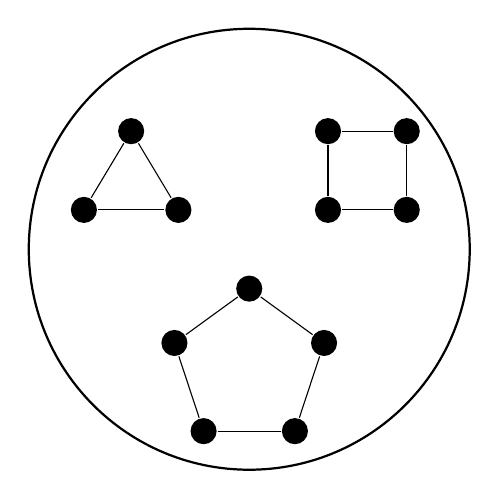
\begin{tikzpicture}
		   \begin{scope}
			   \node (0) at (-2.1, 0)[point] {};
			   \node (1) at (-1.5, 1)[point] {};
			   \node (2) at (-0.9, 0)[point] {};

			   \node (3) at (1, 0)[point] {};
			   \node (4) at (1, 1)[point] {};
			   \node (5) at (2, 1)[point] {};
			   \node (6) at (2, 0)[point] {};

			   \node (7) at (-0.58, -2.81)[point] {};
			   \node (8) at (0.58, -2.81)[point] {};
			   \node (9) at (0.95, -1.69)[point] {};
			   \node (10) at (0, -1)[point] {};
			   \node (11) at (-0.95, -1.69)[point] {};
		   \end{scope}
		   \begin{scope}
			   \path [-] (0) edge (1);
			   \path [-] (1) edge (2);
			   \path [-] (2) edge (0);

			   \path [-] (3) edge (4);
			   \path [-] (4) edge (5);
			   \path [-] (5) edge (6);
			   \path [-] (6) edge (3);

			   \path [-] (7) edge (8);
			   \path [-] (8) edge (9);
			   \path [-] (9) edge (10);
			   \path [-] (10) edge (11);
			   \path [-] (11) edge (7);
		   \end{scope}
		   \draw [thick] (0, -0.5) circle (2.8);
	   \end{tikzpicture}
	   \hspace{20pt}
	   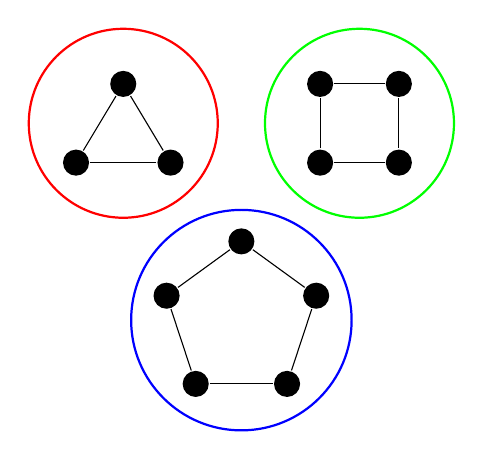
\begin{tikzpicture}
		   \begin{scope}
			   \node (0) at (-2.1, 0)[point] {};
			   \node (1) at (-1.5, 1)[point] {};
			   \node (2) at (-0.9, 0)[point] {};

			   \node (3) at (1, 0)[point] {};
			   \node (4) at (1, 1)[point] {};
			   \node (5) at (2, 1)[point] {};
			   \node (6) at (2, 0)[point] {};

			   \node (7) at (-0.58, -2.81)[point] {};
			   \node (8) at (0.58, -2.81)[point] {};
			   \node (9) at (0.95, -1.69)[point] {};
			   \node (10) at (0, -1)[point] {};
			   \node (11) at (-0.95, -1.69)[point] {};
		   \end{scope}
		   \begin{scope}
			   \path [-] (0) edge (1);
			   \path [-] (1) edge (2);
			   \path [-] (2) edge (0);

			   \path [-] (3) edge (4);
			   \path [-] (4) edge (5);
			   \path [-] (5) edge (6);
			   \path [-] (6) edge (3);

			   \path [-] (7) edge (8);
			   \path [-] (8) edge (9);
			   \path [-] (9) edge (10);
			   \path [-] (10) edge (11);
			   \path [-] (11) edge (7);
		   \end{scope}
		   \draw [thick, color=red] (-1.5, 0.5) circle (1.2);
		   \draw [thick, color=green] (1.5, 0.5) circle (1.2);
		   \draw [thick, color=blue] (0, -2) circle (1.4);
	   \end{tikzpicture}
	   \caption{Levo je prikazana particija usled standardne procedure
	   profinjavanja. Količnički graf sadrži jedan čvor $c$ i važi $\psi_Q(c, c)
	   = 2$. Desno je prikazana particija usled profinjavanja sa invarijantom
	   najkraćeg puta. Količnički graf sadrži tri čvora {\color{red}$a$},
	   {\color{green}$b$} i {\color{blue}$c$} i važi $\psi_Q( a, a) = \{0, 1,
	   1\}$, $\psi_Q(b, b) = \{0, 1, 1, 2\}$ i $\psi_Q(c, c) = \{0, 1, 1, 2, 2\}$,
	   dok su $\psi_Q(x, y)$ za različite $x$ i $y$ multiskupovi sa različitim
	   brojem beskonačnosti.}
	   \label{img:graphinv}
   \end{figure}

   Napomenimo da u radu \cite{McKay} i detaljnije u \cite{nug} postoji uveden
   sličan pojam invarijante grafa koji svakom čvoru (nasuprot parovima čvorova
   u našoj definiciji) obojenog grafa dodeljuje neku vrednost. Ovake
   invarijante se mogu koristiti za dodatno profinjavanje bojenja, najčešće u
   prvih nekoliko nivoa stabla pretrage. Ističemo činjenicu da njima nije
   moguće efektivno pojačati samu proceduru profinjavanja.

% ------------------------------------------------------------------------------
\chapter{Rezultati}
% ------------------------------------------------------------------------------

  U ovoj glavi prikazani su rezultati vremena izvršavanja implementacije
  algoritma na raznim klasama grafova. Algoritam je implementiran u programskom
  jeziku \CC\ u okviru programa \emph{morphi}. Izvorni kod je dostupan na
  adresi \url{https://github.com/idrecun/morphi}.  Testiranje je vršeno na
  grafovima iz kolekcije programa \emph{bliss} i na nekoliko klasa
  nasumično generisanih grafova. Svi grafovi preuzeti su sa
  \url{https://pallini.di.uniroma1.it/Graphs.html}.

  \section{Detalji testiranja}

	U rezultatima prikazano je vreme izvršavanja programa mereno komandom
	\emph{time} ugrađenom u \emph{Bash}, kao zbir vremena koje je program
	proveo u korisničkom i sistemskom režimu. Granica za vreme izvršavanja je u
	svim primerima postavljena na 100 sekundi. Testiranje je vršeno na HP
	Spectre x360 laptop računaru sa Intel i5 procesorom. U trenutku testiranja
	implementacija nije podržavala izvršavanje na više procesorskih jezgara.

	Testirane su dve varijante algoritma. U prvoj je za invarijantu grafa uzeta
	matrica povezanosti, dok je u drugoj korišćena invarijanta najkraćeg puta
	iz primera \ref{ex:graphinv}. Poređenja radi su prikazani rezultati vremena
	izvršavanja programa \emph{nauty} (na mestima gde je značajno i sa
	upotrebom invarijante najkraćeg puta opisane u \cite{nug}) i \emph{Traces}
	na istim primerima. Za \emph{nauty} su za svaku klasu grafova prikazani
	rezultati za onu reprezentaciju grafa (normalna ili proređena) koja je dala
	bolje rezultate. Horizontalna osa grafika predstavlja broj čvorova grafa, a
	vertikalna osa vreme izvršavanja u sekundama (na logaritamskoj skali).

	\pagebreak

  \section{Nasumično generisani grafovi}

	U ovom odeljku su prikazani rezultati testiranja na klasama nasumično
	generisanih grafova navedenih u nastavku. Rezultati za klasu
	\emph{rnd-3-reg} bez upotrebe invarijante razdaljine nisu prikazani zato
	što za većinu primera program nije prekinuo izvršavanje pre granice od 100
	sekundi.
	\begin{itemize}
		\item \emph{rantree} - Stabla
		\item \emph{ran2} - Grafovi sa verovatnoćom grane $\frac{1}{2}$
		\item \emph{ran10} - Grafovi sa verovatnoćom grane $\frac{1}{10}$
		\item \emph{ransq} - Grafovi sa verovatnoćom grane $\frac{1}{\sqrt{n}}$ za $n$ čvorova
		\item \emph{ranreg} - Regularni grafovi
		\item \emph{rnd-3-reg} - 3-regularni grafovi (iz \emph{bliss} kolekcije)
	\end{itemize}

	U klasama slučajnih grafova bez strukture \emph{ran2}, \emph{ran10} i
	\emph{ransq} složenost pretprocesiranja invarijante grafa najkraćeg puta
	dominira. Pojačanje procedure profinjavanja je za ove primere zanemarljivo
	- na skoro svim primerima se i bez upotrebe dodatne invarijante grafa
	generiše samo jedan čvor stabla pretrage. Upotreba invarijante je
	nepotrebna i u slučaju nasumično generisanih stabala \emph{rantree}.
	Složenost algoritma na primerima ove klase proizilazi pretežno iz pretrage.

	Slučaj klasa regularnih grafova \emph{ranreg} i \emph{rnd-3-reg} je
	drugačiji. Osnovni algoritam se na njima pokazao izuzetno neefikasnim.
	Upotrebom invarijante najkraćeg puta se ova neefikasnost zaobilazi time što
	pojačanje procedure profinjavanja dovodi do generisanja stabla pretrage
	koje sadrži jedan čvor. Rezultat ovoga je da vreme izvršavanja nije
	značajno sporije od vremena izvršavanja programa \emph{nauty}.

	\begin{figure}[!h]
	\center
    \begin{tikzpicture}
		\begin{axis}[
				title={\emph{rantree}},
				ymode=log,
				xmajorgrids=true,
				ymajorgrids=true,
				grid style=dashed,
				cycle list name=mylist
			]

			\addplot
				table{data/rantree.csv};

			\addplot
				table{data/rantree-d.csv};

			\addplot
				table{data/nauty/nauty-rantree-As.csv};

			%\addplot
			%	table{data/nauty/nauty-rantree-As-d.csv};
			\addplot table{};

			\addplot
				table{data/nauty/nauty-rantree-At.csv};

		\end{axis}
	\end{tikzpicture}
    \begin{tikzpicture}
		\begin{axis}[
				title={\emph{ran2}},
				ymode=log,
				xmajorgrids=true,
				ymajorgrids=true,
				grid style=dashed,
				cycle list name=mylist
			]

			\addplot
				table{data/ran2.csv};

			\addplot
				table{data/ran2-d.csv};

			\addplot
				table{data/nauty/nauty-ran2-An.csv};

			%\addplot
			%	table{data/nauty/nauty-ran2-An-d.csv};
			\addplot table{};

			\addplot
				table{data/nauty/nauty-ran2-At.csv};

		\end{axis}
	\end{tikzpicture}

    \begin{tikzpicture}
		\begin{axis}[
				title={\emph{ran10}},
				ymode=log,
				xmajorgrids=true,
				ymajorgrids=true,
				grid style=dashed,
				cycle list name=mylist
			]

			\addplot
				table{data/ran10.csv};

			\addplot
				table{data/ran10-d.csv};

			\addplot
				table{data/nauty/nauty-ran10-An.csv};

			%\addplot
				%table{data/nauty/nauty-ran10-An-d.csv};
			\addplot table{};

			\addplot
				table{data/nauty/nauty-ran10-At.csv};

		\end{axis}
	\end{tikzpicture}
    \begin{tikzpicture}
		\begin{axis}[
				title={\emph{ransq}},
				ymode=log,
				xmajorgrids=true,
				ymajorgrids=true,
				grid style=dashed,
				cycle list name=mylist
			]

			\addplot
				table{data/ransq.csv};

			\addplot
				table{data/ransq-d.csv};

			\addplot
				table{data/nauty/nauty-ransq-As.csv};

			%\addplot
				%table{data/nauty/nauty-ransq-As-d.csv};
			\addplot table{};

			\addplot
				table{data/nauty/nauty-ransq-At.csv};

		\end{axis}
	\end{tikzpicture}
	\end{figure}

	\begin{figure}[!h]
		\center
		\begin{tikzpicture}
			\begin{axis}[
					hide axis,
					xmin=0,
					xmax=1,
					ymin=0,
					ymax=1,
					grid style=dashed,
					cycle list name=mylist,
					legend columns=5
				]
				\addlegendimage{cyan!80!black,mark=square*}
				\addlegendentry{\small morphi}
				\addlegendimage{red!90!black,mark=square*}
				\addlegendentry{\small morphi/inv}
				\addlegendimage{blue,mark=*}
				\addlegendentry{\small nauty}
				\addlegendimage{orange,mark=*}
				\addlegendentry{\small nauty/inv}
				\addlegendimage{green!80!black,mark=diamond*}
				\addlegendentry{\small Traces}
			\end{axis}
		\end{tikzpicture}
	\end{figure}
	\begin{figure}[!h]
	\center
    \begin{tikzpicture}
		\begin{axis}[
				title={\emph{ranreg}},
				ymode=log,
				xmajorgrids=true,
				ymajorgrids=true,
				grid style=dashed,
				cycle list name=mylist
			]

			\addplot
				table{data/ranreg.csv};

			\addplot
				table{data/ranreg-d.csv};

			\addplot
				table{data/nauty/nauty-ranreg-As.csv};

			\addplot
				table{data/nauty/nauty-ranreg-As-d.csv};

			\addplot
				table{data/nauty/nauty-ranreg-At.csv};

		\end{axis}
	\end{tikzpicture}
    \begin{tikzpicture}
		\begin{axis}[
				title={\emph{rnd-3-reg}},
				ymode=log,
				xmajorgrids=true,
				ymajorgrids=true,
				grid style=dashed,
				cycle list name=mylist
			]

			\addplot table{};

			\addplot
				table{data/rnd-3-reg-d.csv};

			\addplot
				table{data/nauty/nauty-rnd-3-reg-As.csv};

			\addplot
				table{data/nauty/nauty-rnd-3-reg-As-d.csv};

			\addplot
				table{data/nauty/nauty-rnd-3-reg-At.csv};

		\end{axis}
	\end{tikzpicture}
	\end{figure}
    
  \section{Grafovi donje granice nekih algoritama}

	Jedno uopštenje klasifikacije čvorova procedurom profinjavanja je
	\emph{k}-dimenzioni WL-metod koji služi za klasifikaciju uređenih $k$-torki
	čvorova grafa i koji se može koristiti za ispitivanje izomorfizma dva
	grafa. Klasa \emph{cfi} iz \emph{bliss} kolekcije je klasa grafova opisanih
	kao težak primer za \emph{k}-dimenzioni WL-metod po tome da je neophodno
	odabrati $k = \Omega(n)$ kako bi korektnost ispitivanja izomorfizma para
	grafova sa $n$ čvorova bila zagarantovana \cite{CFI}.  Rezultati pokazuju
	da je upotrebom invarijante najkraćeg puta moguće ostvariti vreme
	izvršavanje koje je u većini slučajeva za nijansu brže od \emph{nauty}-a
	bez upotrebe invarijante, ali idalje sporije od drugih varijanti programa
	\emph{nauty} i \emph{Traces}.

	\begin{figure}[!h]
	\center
    \begin{tikzpicture}
		\begin{axis}[
				width=10cm,
				title={\emph{cfi}},
				ymode=log,
				xmajorgrids=true,
				ymajorgrids=true,
				grid style=dashed,
				cycle list name=mylist
			]

			\addplot
				table{data/cfi.csv};

			\addplot
				table{data/cfi-d.csv};

			\addplot
				table{data/nauty/nauty-cfi-As.csv};

			\addplot
				table{data/nauty/nauty-cfi-As-d.csv};

			\addplot
				table{data/nauty/nauty-cfi-At.csv};

		\end{axis}
	\end{tikzpicture}
	\end{figure}

	Klase \emph{mz}, \emph{cmz}, \emph{mz-aug}, \emph{mz-aug2} su zasnovane na
	klasi \emph{Mijazakijevih grafova} opisanih kao teški primeri za Mekejev
	algoritam \cite{Miyazaki} koji je centralna tema ovog rada.  Osnovni
	algoritam implementiran u okviru \emph{morphi}-a se na primerima ovih klasa
	ponaša slično \emph{nauty}-u, izuzev u klasi \emph{mz-aug} gde je složenost
	algoritma znatno veća. Na ovim primerima do izražaja dolazi ojačanje
	procedure profinjavanja usled upotrebe invarijante najkraćeg puta, posebno
	u klasama \emph{cmz} i \emph{mz-aug2} gde obe varijante \emph{nauty}-a
	pokazuju eksponencijalno ponašanje koje \emph{morphi} izbegava. Ovo nije
	neočekivano pošto su Mijazakijevi grafovi težak primer za upravo onaj
	algoritam koji \emph{nauty} i osnovna verzija \emph{morphi}-a
	implementiraju i pošto dodatna invarijanta menja taj algoritam na ključnom
	mestu.

	\begin{figure}[!h]
	\center
    \begin{tikzpicture}
		\begin{axis}[
				title={\emph{mz}},
				ymode=log,
				xmajorgrids=true,
				ymajorgrids=true,
				grid style=dashed,
				cycle list name=mylist
			]

			\addplot
				table{data/mz.csv};

			\addplot
				table{data/mz-d.csv};

			\addplot
				table{data/nauty/nauty-mz-As.csv};

			\addplot
				table{data/nauty/nauty-mz-As-d.csv};

			\addplot
				table{data/nauty/nauty-mz-At.csv};

		\end{axis}
	\end{tikzpicture}
    \begin{tikzpicture}
		\begin{axis}[
				title={\emph{cmz}},
				ymode=log,
				xmajorgrids=true,
				ymajorgrids=true,
				grid style=dashed,
				cycle list name=mylist
			]

			\addplot
				table{data/cmz.csv};

			\addplot
				table{data/cmz-d.csv};

			\addplot
				table{data/nauty/nauty-cmz-As.csv};

			\addplot
				table{data/nauty/nauty-cmz-As-d.csv};

			\addplot
				table{data/nauty/nauty-cmz-At.csv};

		\end{axis}
	\end{tikzpicture}

    \begin{tikzpicture}
		\begin{axis}[
				title={\emph{mz-aug}},
				ymode=log,
				xmajorgrids=true,
				ymajorgrids=true,
				grid style=dashed,
				cycle list name=mylist
			]

			\addplot
				table{data/mz-aug.csv};

			\addplot
				table{data/mz-aug-d.csv};

			\addplot
				table{data/nauty/nauty-mz-aug-As.csv};

			\addplot
				table{data/nauty/nauty-mz-aug-As-d.csv};

			\addplot
				table{data/nauty/nauty-mz-aug-At.csv};

		\end{axis}
	\end{tikzpicture}
    \begin{tikzpicture}
		\begin{axis}[
				title={\emph{mz-aug2}},
				ymode=log,
				xmajorgrids=true,
				ymajorgrids=true,
				grid style=dashed,
				cycle list name=mylist
			]

			\addplot
				table{data/mz-aug2.csv};

			\addplot
				table{data/mz-aug2-d.csv};

			\addplot
				table{data/nauty/nauty-mz-aug2-As.csv};

			\addplot
				table{data/nauty/nauty-mz-aug2-As-d.csv};

			\addplot
				table{data/nauty/nauty-mz-aug2-At.csv};

		\end{axis}
	\end{tikzpicture}
	\end{figure}

  \section{Mreže}

	Grafovi klase \emph{grid} su grafovi koordinatnih mreža u dve i tri
	dimenzije. Grafovi klase \emph{grid-sw} su isti ti grafovi sa razmenjenim
	parovima nekih grana. \emph{triang} predstavlja klasu trougaonih grafova.
	Još mreža nalazi se u klasi \emph{lattice}. Rezultati pokazuju da nema
	značajne razlike između dve varijante \emph{morphi}-a. \emph{nauty} i
	\emph{Traces} su na primerima ove klase znatno brži. Jedan od mogućih
	razloga za to je što \emph{morphi} u trenutku testiranja nije podržavao
	odvojenu strukturu podataka za rad sa proređenim grafovima, koja je za ove
	klase korišćena u \emph{nauty}-u.

	\begin{figure}[!h]
	\center
    \begin{tikzpicture}
		\begin{axis}[
				title={\emph{grid}},
				ymode=log,
				xmajorgrids=true,
				ymajorgrids=true,
				grid style=dashed,
				cycle list name=mylist
			]

			\addplot
				table{data/grid.csv};

			\addplot
				table{data/grid-d.csv};

			\addplot
				table{data/nauty/nauty-grid-As.csv};

			%\addplot
				%table{data/nauty/nauty-grid-As-d.csv};
			\addplot table{};

			\addplot
				table{data/nauty/nauty-grid-At.csv};

		\end{axis}
	\end{tikzpicture}
    \begin{tikzpicture}
		\begin{axis}[
				title={\emph{grid-sw}},
				ymode=log,
				xmajorgrids=true,
				ymajorgrids=true,
				grid style=dashed,
				cycle list name=mylist
			]

			\addplot
				table{data/grid-w.csv};

			\addplot
				table{data/grid-w-d.csv};

			\addplot
				table{data/nauty/nauty-grid-w-As.csv};

			%\addplot
				%table{data/nauty/nauty-grid-w-As-d.csv};
			\addplot table{};

			\addplot
				table{data/nauty/nauty-grid-w-At.csv};

		\end{axis}
	\end{tikzpicture}
	\end{figure}

	\begin{figure}[!h]
		\center
		\begin{tikzpicture}
			\begin{axis}[
					hide axis,
					xmin=0,
					xmax=1,
					ymin=0,
					ymax=1,
					grid style=dashed,
					cycle list name=mylist,
					legend columns=5
				]
				\addlegendimage{cyan!80!black,mark=square*}
				\addlegendentry{\small morphi}
				\addlegendimage{red!90!black,mark=square*}
				\addlegendentry{\small morphi/inv}
				\addlegendimage{blue,mark=*}
				\addlegendentry{\small nauty}
				\addlegendimage{orange,mark=*}
				\addlegendentry{\small nauty/inv}
				\addlegendimage{green!80!black,mark=diamond*}
				\addlegendentry{\small Traces}
			\end{axis}
		\end{tikzpicture}
	\end{figure}
	\begin{figure}[!h]
	\center
    \begin{tikzpicture}
		\begin{axis}[
				title={\emph{lattice}},
				ymode=log,
				xmajorgrids=true,
				ymajorgrids=true,
				grid style=dashed,
				cycle list name=mylist
			]

			\addplot
				table{data/lattice.csv};

			\addplot
				table{data/lattice-d.csv};

			\addplot
				table{data/nauty/nauty-lattice-As.csv};

			%\addplot
				%table{data/nauty/nauty-lattice-As-d.csv};
			\addplot table{};

			\addplot
				table{data/nauty/nauty-lattice-At.csv};

		\end{axis}
	\end{tikzpicture}
    \begin{tikzpicture}
		\begin{axis}[
				title={\emph{triang}},
				ymode=log,
				xmajorgrids=true,
				ymajorgrids=true,
				grid style=dashed,
				cycle list name=mylist
			]

			\addplot
				table{data/triang.csv};

			\addplot
				table{data/triang-d.csv};

			\addplot
				table{data/nauty/nauty-triang-As.csv};

			%\addplot
				%table{data/nauty/nauty-triang-As-d.csv};
			\addplot table{};

			\addplot
				table{data/nauty/nauty-triang-At.csv};

		\end{axis}
	\end{tikzpicture}
	\end{figure}

  \section{Grafovi nekih kombinatornih objekata}

	U ovom odeljku su prikazani rezultati testiranja na klasama grafova iz
	\emph{bliss} kolekcije navedenih u nastavku.
	\begin{itemize}
		\item \emph{ag} - Grafovi afine geometrije
		\item \emph{had} - Grafovi Adamarovih matrica
		\item \emph{latin} - Grafovi latinskih kvadrata
		\item \emph{latin-sw} - Grafovi latinskih kvadrata sa razmenjenim parovima grana
		\item \emph{k} - Kompletni grafovi
		\item \emph{paley} - Pejlijevi grafovi
		\item \emph{pg} - Grafovi Dezargovih ravni
		\item \emph{sts} - Grafovi Štajnerovih sistema trojki
		\item \emph{sts-sw} - Grafovi Štajnerovih sistema trojki sa razmenjenim parovima grana
	\end{itemize}
	Pored navedenih klasa, u \emph{bliss} kolekciji postoje i klase
	\emph{had-sw}, \emph{kef} i \emph{pp}. Rezultati za klasu \emph{had-sw}
	nisu prikazani zato što za većinu primera program nije prekinuo izvršavanje
	pre granice od 100 sekundi. Rezultati za klase obojenih grafova \emph{kef}
	i \emph{pp} nisu prikazani zato što prilikom testiranja implementacija nije
	podržavala unošenje obojenih grafova.

	Upotreba invarijante najkraćeg puta ima različite posledice na vreme
	izvršavanja. Na primerima klase \emph{pg} je usporenje najosetnije, dok se
	najznačajnije ubrzanje postiže za primere klase \emph{ag}. Programi
	\emph{nauty} i \emph{Traces} na velikom broju klasa postižu očekivano bolje
	rezultate i ostavljaju prostor za poboljšanje implementacije
	\emph{morphi}-a.

	\pagebreak

	\begin{figure}[!h]
		\center
		\begin{tikzpicture}
			\begin{axis}[
					hide axis,
					xmin=0,
					xmax=1,
					ymin=0,
					ymax=1,
					grid style=dashed,
					cycle list name=mylist,
					legend columns=5
				]
				\addlegendimage{cyan!80!black,mark=square*}
				\addlegendentry{\small morphi}
				\addlegendimage{red!90!black,mark=square*}
				\addlegendentry{\small morphi/inv}
				\addlegendimage{blue,mark=*}
				\addlegendentry{\small nauty}
				\addlegendimage{orange,mark=*}
				\addlegendentry{\small nauty/inv}
				\addlegendimage{green!80!black,mark=diamond*}
				\addlegendentry{\small Traces}
			\end{axis}
		\end{tikzpicture}
	\end{figure}
	\begin{figure}[!h]
	\center
    \begin{tikzpicture}
		\begin{axis}[
				title={\emph{ag}},
				ymode=log,
				xmajorgrids=true,
				ymajorgrids=true,
				grid style=dashed,
				cycle list name=mylist
			]

			\addplot
				table{data/ag.csv};

			\addplot
				table{data/ag-d.csv};

			\addplot
				table{data/nauty/nauty-ag-As.csv};

			%\addplot
				%table{data/nauty/nauty-ag-As-d.csv};
			\addplot table{};

			\addplot
				table{data/nauty/nauty-ag-At.csv};

		\end{axis}
	\end{tikzpicture}
    \begin{tikzpicture}
		\begin{axis}[
				title={\emph{pg}},
				ymode=log,
				xmajorgrids=true,
				ymajorgrids=true,
				grid style=dashed,
				cycle list name=mylist
			]

			\addplot
				table{data/pg.csv};

			\addplot
				table{data/pg-d.csv};

			\addplot
				table{data/nauty/nauty-pg-As.csv};

			%\addplot
				%table{data/nauty/nauty-pg-As-d.csv};
			\addplot table{};

			\addplot
				table{data/nauty/nauty-pg-At.csv};

		\end{axis}
	\end{tikzpicture}

    \begin{tikzpicture}
		\begin{axis}[
				title={\emph{latin}},
				ymode=log,
				xmajorgrids=true,
				ymajorgrids=true,
				grid style=dashed,
				cycle list name=mylist
			]

			\addplot
				table{data/latin.csv};

			\addplot
				table{data/latin-d.csv};

			\addplot
				table{data/nauty/nauty-latin-As.csv};

			%\addplot
				%table{data/nauty/nauty-latin-As-d.csv};
			\addplot table{};

			\addplot
				table{data/nauty/nauty-latin-At.csv};

		\end{axis}
	\end{tikzpicture}
    \begin{tikzpicture}
		\begin{axis}[
				title={\emph{latin-sw}},
				ymode=log,
				xmajorgrids=true,
				ymajorgrids=true,
				grid style=dashed,
				cycle list name=mylist
			]

			\addplot
				table{data/latin-sw.csv};

			\addplot
				table{data/latin-sw-d.csv};

			\addplot
				table{data/nauty/nauty-latin-sw-As.csv};

			%\addplot
				%table{data/nauty/nauty-latin-sw-As-d.csv};
			\addplot table{};

			\addplot
				table{data/nauty/nauty-latin-sw-At.csv};

		\end{axis}
	\end{tikzpicture}

    \begin{tikzpicture}
		\begin{axis}[
				title={\emph{k}},
				ymode=log,
				xmajorgrids=true,
				ymajorgrids=true,
				grid style=dashed,
				cycle list name=mylist
			]

			\addplot
				table{data/k.csv};

			\addplot
				table{data/k-d.csv};

			\addplot
				table{data/nauty/nauty-k-An.csv};

			%\addplot
				%table{data/nauty/nauty-k-An-d.csv};
			\addplot table{};

			\addplot
				table{data/nauty/nauty-k-At.csv};

		\end{axis}
	\end{tikzpicture}
    \begin{tikzpicture}
		\begin{axis}[
				title={\emph{paley}},
				ymode=log,
				xmajorgrids=true,
				ymajorgrids=true,
				grid style=dashed,
				cycle list name=mylist
			]

			\addplot
				table{data/paley.csv};

			\addplot
				table{data/paley-d.csv};

			\addplot
				table{data/nauty/nauty-paley-An.csv};

			%\addplot
				%table{data/nauty/nauty-paley-An-d.csv};
			\addplot table{};

			\addplot
				table{data/nauty/nauty-paley-At.csv};

		\end{axis}
	\end{tikzpicture}
	\end{figure}

	\pagebreak

	\begin{figure}[!h]
		\center
		\begin{tikzpicture}
			\begin{axis}[
					hide axis,
					xmin=0,
					xmax=1,
					ymin=0,
					ymax=1,
					grid style=dashed,
					cycle list name=mylist,
					legend columns=5
				]
				\addlegendimage{cyan!80!black,mark=square*}
				\addlegendentry{\small morphi}
				\addlegendimage{red!90!black,mark=square*}
				\addlegendentry{\small morphi/inv}
				\addlegendimage{blue,mark=*}
				\addlegendentry{\small nauty}
				\addlegendimage{orange,mark=*}
				\addlegendentry{\small nauty/inv}
				\addlegendimage{green!80!black,mark=diamond*}
				\addlegendentry{\small Traces}
			\end{axis}
		\end{tikzpicture}
	\end{figure}
	\begin{figure}[!h]
	\center
    \begin{tikzpicture}
		\begin{axis}[
				title={\emph{sts}},
				ymode=log,
				xmajorgrids=true,
				ymajorgrids=true,
				grid style=dashed,
				cycle list name=mylist
			]

			\addplot[color=cyan!80!black,mark=asterisk]
				table{data/sts.csv};

			\addplot[color=red!90!black,mark=asterisk]
				table{data/sts-d.csv};

			\addplot
				table{data/nauty/nauty-sts-As.csv};

			%\addplot
				%table{data/nauty/nauty-sts-As-d.csv};
			\addplot table{};

			\addplot
				table{data/nauty/nauty-sts-At.csv};

			\addplot[color=cyan!80!black,only marks,mark=square*]
				table{data/sts-good.csv};

			\addplot[color=red!90!black,only marks,mark=square*]
				table{data/sts-d-good.csv};

		\end{axis}
	\end{tikzpicture}
    \begin{tikzpicture}
		\begin{axis}[
				title={\emph{sts-sw}},
				ymode=log,
				xmajorgrids=true,
				ymajorgrids=true,
				grid style=dashed,
				cycle list name=mylist
			]

			\addplot
				table{data/sts-sw.csv};

			\addplot
				table{data/sts-sw-d.csv};

			\addplot
				table{data/nauty/nauty-sts-sw-As.csv};

			%\addplot
				%table{data/nauty/nauty-sts-sw-As-d.csv};
			\addplot table{};

			\addplot
				table{data/nauty/nauty-sts-sw-At.csv};

		\end{axis}
	\end{tikzpicture}

    \begin{tikzpicture}
		\begin{axis}[
				width=10cm,
				title={\emph{had}},
				ymode=log,
				xmajorgrids=true,
				ymajorgrids=true,
				grid style=dashed,
				cycle list name=mylist
			]

			\addplot[color=cyan!80!black,mark=asterisk]
				table{data/had.csv};

			\addplot[color=red!90!black,mark=asterisk]
				table{data/had-d.csv};

			\addplot[color=blue,mark=asterisk]
				table{data/nauty/nauty-had-As.csv};

			%\addplot
				%table{data/nauty/nauty-had-As-d.csv};
			\addplot table{};

			\addplot[color=green,mark=asterisk]
				table{data/nauty/nauty-had-At.csv};

			\addplot[color=cyan!80!black,only marks,mark=square*]
				table{data/had-good.csv};

			\addplot[color=red!90!black,only marks,mark=square*]
				table{data/had-d-good.csv};

			\addplot[color=blue,only marks,mark=*]
				table{data/nauty/nauty-had-As-good.csv};

			%\addplot[color=orange,only marks,mark=diamond]
				%table{data/nauty/nauty-had-As-d-bad.csv};

			\addplot[color=green,only marks,mark=diamond*]
				table{data/nauty/nauty-had-At-good.csv};

		\end{axis}
	\end{tikzpicture}
	\end{figure}


% ------------------------------------------------------------------------------
\chapter{Zaključak i dalji rad}
% ------------------------------------------------------------------------------

  Cilj ovog rada bio je izučavanje i opis savremenog okvira za konstrukciju
  algoritma za ispitivanje izomorfizma grafova. Konstruisan je i implementiran
  algoritam zasnovan na tom okviru i prikazani su rezultati vremena izvršavanja
  implementiranog algoritma na reprezentativnom skupu ulaza. Uvedeno je
  uopštenje algoritma variranjem korišćene invarijante grafa. Rezultati
  testiranja pokazali su da algoritam može biti značajno optimizovan na nekim
  klasama grafova korišćenjem tog uopštenja.

  Postoji više mogućih pravaca za dalji rad. Jedan od njih podrazumeva analizu
  i implementaciju efikasnijih struktura podataka i dodatnih optimizacija sa
  svrhom poboljšanja vremena izvršavanja programa. Jedna optimizacija koja u
  radu nije obrađena je mogućnost otkrivanja automorfizama u unutrašnjim
  čvorovima stabla pretrage na osnovu specifičnih svojstava bojenja. Još jedna
  optimizacija vezana za automorfizme je određivanje orbita u datom čvoru
  stabla. Dok smo u radu razmatrali samo podskup automorfizama koji stabilizuju
  niz individualizovanih čvorova, moguće je koristiti pametniju strukturu
  podataka poput Šrajer-Sims metoda ili njegove probabalističke varijante
  \cite{Seress}.

  Još jedna oblast od interesa za dalje istraživanje je uvedeni pojam
  invarijante grafa. Pored toga što je moguće konstruisati invarijantu grafa
  koja daje jednaku ili bolju proceduru profinjavanja, postoji još pitanja
  kojima se u radu nismo bavili.  Kako je cilj profinjavanja particionisanje
  čvorova u klase što približnije orbitama čvorova, nameće se pitanje u kojoj
  meri je ovo moguće izvesti u opštem slučaju, odnosno da li postoji
  invarijanta grafa koja proizvoljan graf particioniše tačno u orbite ili makar
  u particiju koja se u odnosu na particiju orbita razlikuje na neki odozgo
  ograničen način. Slično pitanje moguće je postaviti i za određene klase
  grafova, kao što je na primeru prikazano da 2-regularne grafove u potpunosti
  rešava invarijanta razdaljine čvorova.  Još jedno srodno, možda suprotno
  pitanje je da li postoji klasa grafova na kojoj proizvoljna invarijanta grafa
  nije značajno bolja od matrice povezanosti.

  Iako je problem vremenske složenosti sa praktičnog stanovišta rešen, ono što
  ostaje kao otvoren problem je korektnost implementacije i verifikabilnost
  rezultata. Postoje dva moguća pristupa ovom problemu. Jedan podrazumeva
  implementaciju algoritma i formalan dokaz korektnosti te implementacije. Mana
  ovog pristupa je efikasnost ovakvih implementacija koje mogu biti znatno
  sporije u odnosu na implementacije razvijene u nekom nižem jeziku. Drugi
  pristup podrazumeva generisanje sertifikata uz rezultat izvršavanja efikasno
  implementiranog programa. Sertifikat bi po završetku izvršavanja programa
  mogao biti analiziran verifikatorom (programom čija je korektnost dokazana)
  koji bi sertifikat koristio kao svedoka da dokaže da je izlaz programa
  korektan. Cilj je koncipirati sertifikat na taj način da implementacija
  verifikatora, iako pisana u višem programskom jeziku koji omogućava formalan
  dokaz korektnosti, bude efikasnija od implementacije samog rešavača. Na
  primer, program za ispitivanje izomorfizma dva grafa kao sertifikat u slučaju
  da su grafovi izomorfni može koristiti pronađen izomorfizam, dok slučaj
  neizomorfnih grafova nije na isti način trivijalan.

% ------------------------------------------------------------------------------
% Literatura
% ------------------------------------------------------------------------------
\literatura

% ==============================================================================
% Završni deo teze i prilozi
\backmatter
% ==============================================================================

% ------------------------------------------------------------------------------
% Biografija kandidata
\begin{biografija}
	Biografija.
\end{biografija}
% ------------------------------------------------------------------------------

\end{document}
